\documentclass[sort&compress]{svjour3} % onecolumn (standard format)
\usepackage[letterpaper,margin=3cm]{geometry}
\smartqed % flush right qed marks, e.g. at end of proof
\usepackage[utf8]{inputenc}
\usepackage{amsmath}
\usepackage{amsfonts}
\usepackage{amssymb}
\usepackage{listings}
\usepackage{mathrsfs}
\usepackage{newtxtext,newtxmath} % unified Times-compatible text+math font (replaces times+mathpazo)
\usepackage{xcolor}
% Removed: float (only needed for [H], now [htbp] throughout); setspace (unused).
\usepackage{soul}
\usepackage{eucal}
\usepackage{enumerate}
% geometry package removed: svjour3 defines its own page layout
\usepackage[title]{appendix}
\usepackage{array}
\usepackage{calligra}
\usepackage{multirow}
\usepackage{placeins}
\newcolumntype{M}[1]{>{\centering\arraybackslash}m{#1}}

\usepackage[
pdfstartview=XYZ,
bookmarks=true,
colorlinks=true,
linkcolor=blue,
urlcolor=blue,
citecolor=blue,
pdftex,
linktocpage=true, % make the page number as hyperlink in table of content
hyperindex=true
]{hyperref}

\usepackage{subfig}
\usepackage{natbib}
%\setcitestyle{authoryear}
\setcitestyle{numbers}
\setcitestyle{square}
\setcitestyle{comma}
\usepackage[pdftex]{graphicx}
\usepackage{epstopdf}
\usepackage{booktabs}
\usepackage{lineno}
%\linenumbers  % uncomment for review submission
% mathpazo removed: replaced by newtxtext,newtxmath above
\usepackage{tikz}
\usetikzlibrary{shapes.geometric}
\usetikzlibrary{arrows}
\usetikzlibrary{trees}
\usepackage{indentfirst}
\usepackage{caption}
\usepackage{enumitem}
\usepackage[para]{threeparttable}
\usepackage{upgreek}

% Insert the name of "your journal" with
%\journalname{International Journal for Numerical Methods in Engineering}
%\journalname{Propellants, Explosives, Pyrotechnics}
%\journalname{Computational Mechanics}
%\journalname{Granular Matter}
\journalname{Computer Methods in Applied Mechanics and Engineering}

\newcommand{\tensor}[1]{\ensuremath{\boldsymbol{#1}}}
\renewcommand{\vec}[1]{\ensuremath{\boldsymbol{#1}}}
\newcommand{\jump}[1]{\lbrack\!\lbrack #1 \rbrack\!\rbrack}
\newcommand{\alert}[1]{\textcolor{red}{#1}}
\DeclareMathOperator{\grad}{\nabla^{\tensor x}}
\DeclareMathOperator{\diver}{\nabla^{\tensor x}\cdot}
\DeclareMathOperator{\Grad}{\nabla^{\tensor X}}
\DeclareMathOperator{\Diver}{\nabla^{\tensor X}\cdot}
\DeclareMathOperator{\sym}{sym}
\DeclareMathOperator{\skw}{skw}
\DeclareMathOperator{\tr}{tr}
\DeclareMathOperator{\dev}{dev}
\DeclareMathOperator{\sign}{sign}
\DeclareMathOperator{\diag}{diag}
\DeclareMathOperator*{\argmin}{argmin}

\newcommand{\elasCoeff}{C}
\newcommand{\ElasCoeff}{\mathbb{\elasCoeff}}

\DeclareMathOperator{\T}{T}
\DeclareMathOperator{\Identity}{\tensor I}

\newcommand{\length}{L}
\newcommand{\tilt}{T}
\newcommand{\jacDet}{J}
\newcommand{\volume}{V}
\newcommand{\density}{\rho}
\newcommand{\deforGrad}{F}
\newcommand{\cauchyStress}{\sigma}
\newcommand{\firstPKStress}{P}
\newcommand{\secPKStress}{S}
\newcommand{\lagranStrain}{E}
\DeclareMathOperator{\LengthTilt}{\tensor H}
\DeclareMathOperator{\DeforGrad}{\tensor \deforGrad}
\DeclareMathOperator{\CauchyStress}{\tensor \cauchyStress}
\DeclareMathOperator{\FirstPKStress}{\tensor \firstPKStress}
\DeclareMathOperator{\RightCGDefor}{\tensor C}
\DeclareMathOperator{\SecPKStress}{\tensor \secPKStress}
\DeclareMathOperator{\LagranStrain}{\tensor \lagranStrain}

\newcommand{\temp}{T}
\newcommand{\shear}{\gamma}
\newcommand{\pres}{p}

\newcommand{\freeEnergy}{\Psi}
\newcommand{\interEnergy}{U}
\newcommand{\entropy}{\eta}
\newcommand{\specHeat}{c}
\newcommand{\thermStress}{\beta}
\newcommand{\gruneisen}{\Gamma}
\DeclareMathOperator{\ThermStress}{\tensor \thermStress}
\DeclareMathOperator{\Gruneisen}{\tensor \gruneisen}
\DeclareMathOperator{\HeatFlux}{\tensor Q}
\DeclareMathOperator{\ThermExpans}{\tensor \alpha}

\newcommand{\dataDim}{K}
\newcommand{\inputDim}{N}
\newcommand{\func}{f}
\newcommand{\layer}{L}
\newcommand{\activ}{\sigma}
\newcommand{\lossCoeff}{w}
\newcommand{\loss}{\mathcal{L}}
\newcommand{\frobenNorm}{F}
\newcommand{\eigval}{\lambda}
\newcommand{\outputs}{y}
\newcommand{\RealSet}{\mathbb{R}}
\DeclareMathOperator{\Inputs}{\tensor{\mathcal{X}}}
\DeclareMathOperator{\Outputs}{\tensor \outputs}
\DeclareMathOperator{\inputs}{\tensor \chi}
\DeclareMathOperator{\Weight}{\tensor W}
\DeclareMathOperator{\Bias}{\tensor s}
\DeclareMathOperator{\MLP}{MLP}
\DeclareMathOperator{\Param}{\tensor \theta}
\DeclareMathOperator{\Zero}{\tensor 0}
\DeclareMathOperator{\ReLU}{ReLU}

\newcommand{\thermEnergy}{h}

\newcommand{\dataPoint}{c}

\DeclareMathOperator{\SiLU}{SiLU}
\DeclareMathOperator{\softplus}{softplus}

\newcommand{\increStiff}{B}
\newcommand{\IncreStiff}{\mathbb{\increStiff}}
\DeclareMathOperator{\SpatStrain}{\tensor \varepsilon}
\DeclareMathOperator{\MD}{MD}

\usepackage{algorithm}
\usepackage{algpseudocode}
\newcommand\StateX{\Statex\hspace{\algorithmicindent}}
\algdef{SE}[SUBALG]{Indent}{EndIndent}{}{\algorithmicend}
\algtext*{Indent}
\algtext*{EndIndent}

\newtheorem{assumption}{Assumption}
\newcommand*{\affaddr}[1]{#1}
\newcommand*{\affmark}[1][*]{\textsuperscript{#1}}




\begin{document}

\title{Geometry-informed neural atlas for boundary value problems of complex 3D geometries}

\titlerunning{geometry-informed neural charts}

\author{WaiChing Sun \protect\affmark[a]}

\institute{
\affaddr{\affmark[a] Department of Civil Engineering and Engineering Mechanics, Columbia University, New York, NY 10027, USA. \email{wsun@columbia.edu}} \\
%\affaddr{\affmark[b] Terminal Effects Division, DEVCOM Army Research Laboratory, Aberdeen Proving Ground, MD 21005, USA} \\
%\affaddr{\affmark[c] Department of Chemistry and Materials Science \& Engineering Institute, University of Missouri, Columbia, MO 65211, USA} \\
}

\date{Received: [DATE] / Accepted: [DATE]}

\maketitle

\begin{abstract}
This paper presents a geometry-informed neural atlas framework that bypasses conventional volumetric meshing for boundary-value problems on geometrically complex three-dimensional domains. The computational domain is represented by an atlas of overlapping volumetric coordinate charts, each equipped with a learned decoder map and its Jacobian. Governing equations are pulled back to chart-local reference coordinates via the Piola identity, yielding mapped residuals that can be discretized by either physics-informed neural networks (PINNs) or classical finite elements on the same frozen atlas. Chart-local solutions are coupled through multiplicative Schwarz alternating iterations with partition-of-unity blending on overlapping regions. Three benchmark problems of increasing geometric complexity are considered: (i)~an ellipsoid Poisson problem with analytic maps that verifies the mapped differential operator; (ii)~a Stanford Bunny Poisson problem on a learned eight-chart atlas, solved by both a compact PINN and a P1 tetrahedral FEM; and (iii)~a torus inverse problem that recovers constitutive parameters from prescribed kinematics. On the rabbit benchmark the compact PINN achieves a relative $L^2$ error of $2.21\times 10^{-2}$, while the atlas-based FEM recovers the expected $O(h^2)$ convergence rate across five refinement levels and reaches $1.79\times 10^{-2}$ at the finest resolution ($1.48\times 10^{6}$ degrees of freedom). At matched accuracy the two solvers exhibit comparable wall-clock times, but the FEM requires approximately $8.5\times$ fewer neural-network evaluations by caching the geometric precomputation. The results demonstrate that a single frozen atlas can serve as a reusable computational substrate for multiple solver paradigms, decoupling the geometric representation from the PDE discretization strategy.
\end{abstract}

\keywords{coordinate charts, Schwarz method, physics-informed neural networks, meshfree methods, complex geometry}

\section{Introduction} \label{sec:introduction}
Boundary-value problems on complex three-dimensional bodies are still solved most reliably when the geometry can be converted into a solver-ready volumetric discretization. In computational mechanics, that usually means constructing and maintaining a high-quality mesh, together with remeshing, enrichment, or geometry-regularization strategies when the morphology becomes intricate \citep{de_souza_neto_computational_2011,quey_large-scale_2011,moes_finite_1999}. That maturity is a major strength of classical methods, but it also means that geometry preparation can become a substantial numerical task in its own right when the body contains thin features, strongly curved interiors, or interfaces imported from external geometric data. The aim of the present paper is to reduce that geometric bottleneck without discarding the local structure that makes computational mechanics reliable.

Physics-informed neural networks (PINNs) reopen that balance of labor by replacing element-level trial spaces with differentiable surrogates constrained by governing equations and data \citep{raissi2019physicsinformed,vlassis2021sobolev}. Decomposition-based neural solvers further show that local neural models can improve training scalability and approximation quality when the computational domain is partitioned \citep{jagtap2020xpinns,shukla2021parallel,moseley2021fbpinns}. The question driving this paper is therefore more geometric than algorithmic: can the partition itself be promoted to a volumetric atlas that represents the body, supplies local change-of-variables formulas, and organizes overlap coupling without first requiring a conventional volumetric mesh?

\subsection{Position relative to existing literature}
Relative to classical overlapping Schwarz and domain decomposition, the present work borrows the coupling logic but changes the source of the subdomains. Schwarz methods assume local problems posed on overlapping regions and then use boundary or interface exchange to recover a global solution \citep{quarteroni1999domain}. In mainstream computational mechanics, those local regions are usually obtained from a pre-existing discretization infrastructure whose quality has already been secured by meshing and remeshing procedures \citep{de_souza_neto_computational_2011,quey_large-scale_2011}. These methods remain the baseline whenever high-quality volumetric meshes can be generated and maintained efficiently. The difficulty addressed here is the complementary regime in which constructing that solver-ready geometry is itself cumbersome.

Relative to the PINN literature, the distinction is different. Foundational PINN formulations establish meshfree forward and inverse PDE solution \citep{raissi2019physicsinformed}, while decomposition-based variants such as XPINNs, parallel PINNs, and FBPINNs localize the neural approximation to improve scalability, expressivity, or conditioning \citep{jagtap2020xpinns,shukla2021parallel,moseley2021fbpinns}. However, their partitions are introduced primarily to improve optimization and parallel execution rather than to serve as a volumetric geometric atlas. Separate work on neural and implicit geometry representations shows that learned models can recover complex surfaces and level-set structure from data \citep{williams2019deep,chunming_li_level_2005,lee_narrow-band_2014}. Yet surface-faithful reconstruction does not by itself furnish a solver-ready volumetric atlas with overlap maps, chart Jacobians, and transition operators for local PDE evaluation.

The present paper addresses that gap by building the computational pipeline around the atlas itself. The charts are introduced first as the volumetric representation of the body; the mapped PDE operators and Schwarz communication are then defined on top of that representation. In that sense the framework is geometry-informed rather than merely domain-decomposed.

\subsection{Major contributions and scope}
The manuscript makes four bounded contributions relative to the existing literature:
\begin{enumerate}[leftmargin=*]
\item \textbf{Volumetric neural atlas as geometric representation.} The overlapping charts represent the domain itself rather than acting only as an optimization partition, which distinguishes the framework from decomposition-based neural solvers whose subdomains are introduced mainly for training convenience.
\item \textbf{Mapped chart-local PDE solve with Schwarz coupling.} Each governing equation is pulled back to chart-local coordinates and coupled through alternating Schwarz updates, importing domain-decomposition logic into a geometry-first atlas setting without assuming a pre-existing volumetric mesh.
\item \textbf{Bridge from analytic geometry to mesh-derived geometry.} The same workflow supports analytic maps and learned volumetric geometry from PLY/SDF data, so the solver can start from exact benchmark geometry or from externally supplied surface data while retaining interior queries needed for atlas construction and collocation.
\item \textbf{Validated, scope-bounded evidence with classical baseline.} The benchmark set spans analytic verification, a fixed-atlas rabbit forward Poisson solve with both PINN and P1 FEM local solvers, a Stanford Bunny volumetric geometry-learning bridge, and a controlled torus inverse identification problem. The rabbit forward solve is the strongest current evidence; the head-to-head FEM baseline independently validates the mapped-operator formulation through $O(h^2)$ convergence and shows that the atlas is a reusable geometric substrate for multiple discretization strategies. The manuscript does not claim universal superiority over mature mesh-based methods or a fully general nonlinear inverse-field capability.
\end{enumerate}

The paper is organized accordingly. Section~\ref{sec:methodology} introduces the volumetric atlas, the mapped PDE operator, the special-case global-map training used only for simply connected examples, and the Schwarz update on a fixed atlas. Section~\ref{sec:implementation} then records the geometry pipeline, quality-assurance gates, and stabilization heuristics that materially affect the reported benchmarks. Section~\ref{sec:benchmark_formulations} presents the benchmark formulations and numerical evidence, and Section~\ref{sec:discussion} interprets the resulting scope and limitations.

\section{Methodology}
\label{sec:methodology}

Before giving the derivations, we fix the notation used in this section. We use $x$ for a point in the physical body, $\boldsymbol{\zeta}$ for a chart-local reference coordinate on one atlas patch, and $\boldsymbol{\xi}$ for the global reference-ball coordinate used only in the special simply connected examples. This two-level notation is enough for the methodology while avoiding the earlier conflict in which one symbol was asked to represent both a local chart coordinate and a global reference coordinate.

\subsection{Geometric setting: manifold, coordinate charts, and atlas}
\label{sec:atlas_geometry}
Let $\Omega \subset \mathbb{R}^3$ be a bounded body with sufficiently regular boundary $\partial\Omega$. From a computational standpoint, the closure $\overline{\Omega}$ may be viewed as a compact three-dimensional manifold with boundary embedded in the ambient Euclidean space. We use this language only to formalize one practical point: when a single low-distortion volumetric parametrization is unavailable, the same body may still be described by several compatible local volumetric coordinates. The implementation therefore works with a finite computational atlas of bounded patches in $\mathbb{R}^3$, and the manifold viewpoint provides the minimal structure needed to treat those patches as one geometric object.

\subsubsection{Coordinate charts and local coordinates}
A coordinate chart is a pair $(\widehat{\Omega}_i,\varphi_i)$ consisting of a reference patch $\widehat{\Omega}_i\subset\mathbb{R}^3$ and a smooth map from that local coordinate domain into the physical body. In the present work the charts are volumetric rather than surface-valued, because the downstream solver must sample interior collocation points, evaluate volumetric PDE residuals, and communicate information through overlapping subregions. The basic chart family is written as
\begin{equation}
\mathcal{A}=\{(\widehat{\Omega}_i,\varphi_i)\}_{i=1}^{M},
\qquad
\widehat{\Omega}_i \subset \mathbb{R}^3,
\qquad
\varphi_i:\widehat{\Omega}_i \rightarrow \mathbb{R}^3,
\label{eq:atlas_def}
\end{equation}
with physical patches
\begin{equation}
\Omega_i := \varphi_i(\widehat{\Omega}_i),
\qquad
\overline{\Omega}\subset \bigcup_{i=1}^{M}\overline{\Omega}_i.
\label{eq:atlas_cover}
\end{equation}
The Jacobian matrix of chart $i$ is denoted by
\begin{equation}
\mathbf{J}_i(\boldsymbol{\zeta}) := D_{\boldsymbol{\zeta}} \varphi_i(\boldsymbol{\zeta})\in\mathbb{R}^{3\times 3},
\qquad
j_i(\boldsymbol{\zeta}):=\det \mathbf{J}_i(\boldsymbol{\zeta}).
\label{eq:atlas_jac}
\end{equation}
For the mapped PDE derivations below, each chart is assumed locally nondegenerate:
\begin{equation}
j_i(\boldsymbol{\zeta})\ge j_{\min}>0
\qquad \text{for all sampled }\boldsymbol{\zeta}\in \widehat{\Omega}_i.
\label{eq:atlas_nondegenerate}
\end{equation}
This condition guarantees a locally invertible change of variables. It does \emph{not} by itself imply global injectivity. Whenever we refer to a chart inverse
\begin{equation}
\pi_i := \varphi_i^{-1}:\Omega_i\rightarrow \widehat{\Omega}_i,
\label{eq:atlas_inverse}
\end{equation}
we mean the inverse on a patch where the chart is assumed or verified to be injective. In the implementation, positive Jacobian determinant is enforced or monitored at sampled points, while global injectivity is treated as a trained geometric property rather than a theorem following automatically from \eqref{eq:atlas_nondegenerate}.

The rabbit atlas used later in the paper makes this local-coordinate idea concrete. Each chart is anchored at a seed point $s_i$ with an orthonormal local frame $\{t_{1i},t_{2i},n_i\}$, and a physical sample $x$ is first expressed in rigid local coordinates by
\begin{equation}
\boldsymbol{\zeta}^{\mathrm{rig}}_i(x)
:=
\left(
(x-s_i)\cdot t_{1i},
\,
(x-s_i)\cdot t_{2i},
\,
(x-s_i)\cdot n_i
\right).
\label{eq:atlas_rigid_local_coords}
\end{equation}
This is the coordinate transform used in the atlas-training stage and in the rabbit Schwarz solver before the learned decoder adds a bounded residual correction to the rigid frame map. The chart is therefore a local refinement of a simple Euclidean coordinate system, not an unconstrained parametrization trained from scratch.

\subsubsection{Atlas, overlaps, and transition maps}
An atlas is a finite collection of such charts whose physical images cover the body and overlap in a controlled way. In this manuscript the overlap is essential, because it is what later allows neighboring local PDE solves to exchange information without first building a global volumetric mesh. On overlaps we define
\begin{equation}
\Omega_{ij}:=\Omega_i\cap \Omega_j,
\qquad
\widehat{\Omega}_{ij}:=\pi_i(\Omega_{ij})\subset \widehat{\Omega}_i,
\label{eq:atlas_overlap}
\end{equation}
and the transition map
\begin{equation}
\psi_{ij}:=\pi_j\circ \varphi_i:\widehat{\Omega}_{ij}\rightarrow \widehat{\Omega}_j,
\qquad
\varphi_i(\boldsymbol{\zeta})=\varphi_j(\psi_{ij}(\boldsymbol{\zeta})).
\label{eq:atlas_transition}
\end{equation}
The transition map $\psi_{ij}$ identifies the same physical point through two neighboring coordinate systems. It is therefore the object that makes overlap consistency meaningful: if $x\in\Omega_{ij}$ and $x=\varphi_i(\boldsymbol{\zeta})$, then $\psi_{ij}(\boldsymbol{\zeta})$ is the coordinate in chart $j$ representing that same $x$. This local compatibility is the geometric counterpart of the chart-to-chart transmission used later by the alternating Schwarz solver.

The overlaps also define the atlas adjacency graph
\begin{equation}
G_{\mathcal{A}}=(V_{\mathcal{A}},E_{\mathcal{A}}),
\qquad
V_{\mathcal{A}}=\{1,\dots,M\},
\qquad
E_{\mathcal{A}}=\{(i,j):\, i\neq j,\ \Omega_{ij}\neq \emptyset\}.
\label{eq:atlas_overlap_graph}
\end{equation}
This graph is more than bookkeeping. It is the same neighborhood structure later used by the Schwarz sweep and by the graph-coloring that identifies non-overlapping chart groups for limited parallel updates.

When a single global field is needed for post-processing, we use partition-of-unity weights $\{\omega_i\}_{i=1}^{M}$ satisfying
\begin{equation}
\omega_i:\Omega\rightarrow [0,1],
\qquad
\mathrm{supp}(\omega_i)\subset \Omega_i,
\qquad
\sum_{i=1}^{M}\omega_i(x)=1.
\label{eq:atlas_pou}
\end{equation}
For any chart-local quantity $\widehat{g}_i$, the blended global field is
\begin{equation}
g_h(x)=\sum_{i=1}^{M}\omega_i(x)\,\widehat{g}_i(\pi_i(x)).
\label{eq:atlas_blend}
\end{equation}
The atlas therefore serves two roles at once. Geometrically it represents the body by local volumetric parametrizations; algorithmically it provides the overlap graph and the coordinate transformations needed for local residual evaluation and inter-chart communication. In the rabbit implementation, a candidate atlas is accepted only after coverage, overlap-consistency, boundary-fit, and foldover diagnostics pass their prescribed gates, so the local chart structure used by the solver is already screened as a geometric object before PDE training begins.

\begin{table}[htbp]
\centering
\footnotesize
\caption{Notation used in Section~\ref{sec:methodology}. Physical-space variables, chart-local reference variables, and global reference-ball variables are separated explicitly so that the reader can track which coordinate system is active at each step of the derivation.}
\label{tab:notation}
\begin{tabular}{p{2.35cm}p{3.15cm}p{7.05cm}}
\toprule
Group & Symbol & Role in the method \\
\midrule
\multirow{4}{*}{Physical space}
& $\Omega$, $\partial\Omega$ & physical body and its boundary \\
& $x$ & physical-space point used in the governing PDE \\
& $\Omega_i$, $\Omega_{ij}$ & chart image and chart-overlap region in physical space \\
& $u(x),\,u_h(x)$ & physical state field and the blended global field used for reporting \\
\midrule
\multirow{4}{*}{\shortstack[l]{Chart-local\\ reference}}
& $\widehat{\Omega}_i$ & reference patch attached to chart $i$ \\
& $\boldsymbol{\zeta}$ & local coordinate used to evaluate one chart-local network \\
& $\widehat{\Omega}_{ij}$ & overlap region written in the coordinates of chart $i$ \\
& $\widehat{u}_i(\boldsymbol{\zeta})$ & chart-local state field defined on $\widehat{\Omega}_i$ \\
\midrule
\multirow{2}{*}{\shortstack[l]{Global\\ reference ball}}
& $B^3=\{\boldsymbol{\xi}\in\mathbb{R}^3:\|\boldsymbol{\xi}\|<1\}$ & unit ball used only by the special global-map examples \\
& $\Psi_\theta(\boldsymbol{\xi})$ & learned or analytic global map from the reference ball to the physical domain \\
\midrule
\multirow{4}{*}{Map operators}
& $\varphi_i,\pi_i$ & chart map and its local inverse \\
& $\psi_{ij}=\pi_j\circ\varphi_i$ & transition map from chart-$i$ coordinates to chart-$j$ coordinates on an overlap \\
& $\mathbf{J}_i=D_{\boldsymbol{\zeta}}\varphi_i,\; j_i=\det\mathbf{J}_i$ & Jacobian matrix and Jacobian determinant of chart $i$ \\
& $\omega_i$ & partition-of-unity weight used in the global blend \\
\midrule
\shortstack[l]{Shared solver\\ quantities}
& $\eta,\lambda_*$ & $\eta$ denotes global material or inverse parameters; $\lambda_*$ denotes loss weights shared across charts \\
\bottomrule
\end{tabular}
\end{table}

Figure~\ref{fig:atlas_slice} gives a schematic planar slice through this volumetric atlas. The drawing is intentionally geometric rather than algorithmic: it emphasizes that the local reference patches, their physical images, and their overlaps together define the computational body representation used by the later PDE solve.

\begin{figure}[htbp]
\centering
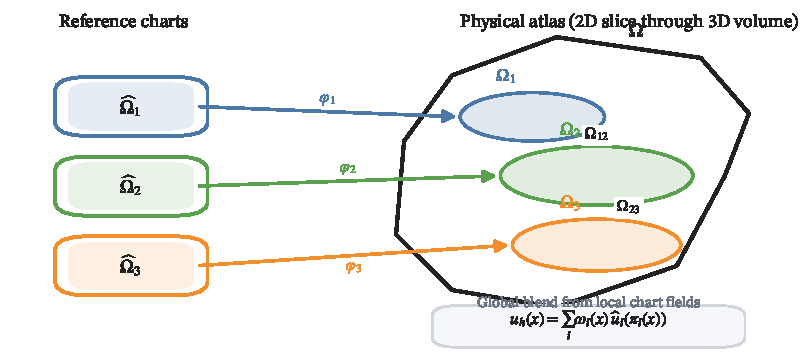
\includegraphics[width=0.98\textwidth]{figures_cmame_core/method/atlas_slice_pub.png}
\caption{Conceptual view of the volumetric neural atlas. The left half shows chart-local reference patches parameterized by $\boldsymbol{\zeta}$; the right half shows their mapped physical images covering overlapping parts of $\Omega$. The arrows represent the chart maps $\varphi_i$, while the lower formula indicates the global blend assembled from the chart-local fields after the local solves are complete. The drawing is a planar slice through a three-dimensional construction, so it illustrates volumetric charts rather than a surface atlas.}
\label{fig:atlas_slice}
\end{figure}

\subsection{Mapped PDE operator on a volumetric chart}
\label{sec:mapped_operator}
Let $u:\Omega\rightarrow\mathbb{R}^{q}$ be the physical state. For vector-valued fields we collect component gradients row-wise, so
\[
\nabla_x u(x)\in \mathbb{R}^{q\times 3}.
\]
We write the physical PDE in divergence form as
\begin{equation}
\nabla_x\cdot \mathcal{G}\!\left(x,u(x),\nabla_x u(x);\eta\right)
+ \mathcal{S}\!\left(x,u(x),\nabla_x u(x);\eta\right)=0
\qquad \text{in }\Omega,
\label{eq:abstract_pde}
\end{equation}
where the divergence acts row-wise and
\[
\mathcal{G}(x,u,\nabla u;\eta)\in \mathbb{R}^{q\times 3},
\qquad
\mathcal{S}(x,u,\nabla u;\eta)\in \mathbb{R}^{q}.
\]
Physical boundary conditions are written as
\begin{equation}
u=u_D \quad \text{on }\Gamma_D,
\qquad
\mathcal{G}(x,u,\nabla_x u;\eta)\,n = t_N
\quad \text{on }\Gamma_N,
\label{eq:abstract_bc}
\end{equation}
with outward unit normal $n$.

On chart $i$, let $\boldsymbol{\zeta}\in\widehat{\Omega}_i$ denote the local reference coordinate and define the pulled-back state by
\begin{equation}
\widehat{u}_i(\boldsymbol{\zeta}):=u(\varphi_i(\boldsymbol{\zeta})).
\label{eq:pullback_state}
\end{equation}
Because gradients are stored row-wise, the chain rule takes the form
\begin{equation}
\nabla_x u(\varphi_i(\boldsymbol{\zeta}))
=
\nabla_{\boldsymbol{\zeta}} \widehat{u}_i(\boldsymbol{\zeta})\,\mathbf{J}_i(\boldsymbol{\zeta})^{-1}.
\label{eq:grad_pullback}
\end{equation}
The physical flux is first evaluated on the chart and then converted to a reference-space flux by the row-wise Piola transform:
\begin{align}
\widehat{\mathcal{G}}_i(\boldsymbol{\zeta};\eta)
&:=
\mathcal{G}\!\left(\varphi_i(\boldsymbol{\zeta}),\widehat{u}_i(\boldsymbol{\zeta}),\nabla_{\boldsymbol{\zeta}} \widehat{u}_i(\boldsymbol{\zeta})\mathbf{J}_i(\boldsymbol{\zeta})^{-1};\eta\right),
\label{eq:pullback_flux}\\
\widehat{\mathcal{P}}_i(\boldsymbol{\zeta};\eta)
&:=
j_i(\boldsymbol{\zeta})\,\widehat{\mathcal{G}}_i(\boldsymbol{\zeta};\eta)\,\mathbf{J}_i(\boldsymbol{\zeta})^{-T}.
\label{eq:piola_flux}
\end{align}
The pulled-back source term is
\begin{equation}
\widehat{\mathcal{S}}_i(\boldsymbol{\zeta};\eta)
:=
\mathcal{S}\!\left(\varphi_i(\boldsymbol{\zeta}),\widehat{u}_i(\boldsymbol{\zeta}),\nabla_{\boldsymbol{\zeta}} \widehat{u}_i(\boldsymbol{\zeta})\mathbf{J}_i(\boldsymbol{\zeta})^{-1};\eta\right).
\label{eq:pullback_source}
\end{equation}
We reserve the notation $\widehat{\mathcal{P}}_i$ for the Piola-transformed flux entering the reference-space divergence and $\widehat{\mathcal{S}}_i$ for the pulled-back source term, so the flux and source roles remain distinct throughout the derivation.
With these definitions, the Piola identity $\nabla_x\cdot\mathcal{G} = j_i^{-1}\,\nabla_{\boldsymbol{\zeta}}\cdot(j_i\,\mathcal{G}\,\mathbf{J}_i^{-T}) = j_i^{-1}\,\nabla_{\boldsymbol{\zeta}}\cdot\widehat{\mathcal{P}}_i$ applied to \eqref{eq:abstract_pde} and multiplied through by $j_i$ yields the mapped residual on the reference chart:
\begin{equation}
\widehat{\mathcal{R}}_i(\boldsymbol{\zeta};\eta)
:=
\nabla_{\boldsymbol{\zeta}}\cdot \widehat{\mathcal{P}}_i(\boldsymbol{\zeta};\eta)
+
j_i(\boldsymbol{\zeta})\,\widehat{\mathcal{S}}_i(\boldsymbol{\zeta};\eta),
\qquad \boldsymbol{\zeta}\in \widehat{\Omega}_i.
\label{eq:mapped_residual}
\end{equation}

For the Dirichlet boundary we use
\begin{equation}
\widehat{\mathcal{B}}_{i,D}(\boldsymbol{\zeta}):=\widehat{u}_i(\boldsymbol{\zeta})-u_D(\varphi_i(\boldsymbol{\zeta})),
\qquad \boldsymbol{\zeta}\in \widehat{\Gamma}_{i,D}:=\pi_i(\Gamma_D\cap \Omega_i).
\label{eq:mapped_dirichlet}
\end{equation}
For Neumann or traction conditions, if $\widehat{n}_i(\boldsymbol{\zeta})$ is a reference outward normal on the relevant portion of $\partial\widehat{\Omega}_i$, the physical normal is
\begin{equation}
n_i(\varphi_i(\boldsymbol{\zeta}))
=
\frac{\mathbf{J}_i(\boldsymbol{\zeta})^{-T}\widehat{n}_i(\boldsymbol{\zeta})}
{\|\mathbf{J}_i(\boldsymbol{\zeta})^{-T}\widehat{n}_i(\boldsymbol{\zeta})\|},
\label{eq:mapped_normal}
\end{equation}
and the pulled-back Neumann residual is
\begin{equation}
\widehat{\mathcal{B}}_{i,N}(\boldsymbol{\zeta};\eta)
:=
\widehat{\mathcal{G}}_i(\boldsymbol{\zeta};\eta)\,n_i(\varphi_i(\boldsymbol{\zeta})) - t_N(\varphi_i(\boldsymbol{\zeta})),
\label{eq:mapped_neumann}
\end{equation}
where $\widehat{\mathcal{G}}_i$ is the physical flux from \eqref{eq:pullback_flux} and $n_i$ is the physical normal from \eqref{eq:mapped_normal}, both evaluated at the chart-mapped point $\varphi_i(\boldsymbol{\zeta})$.

\begin{figure}[htbp]
\centering
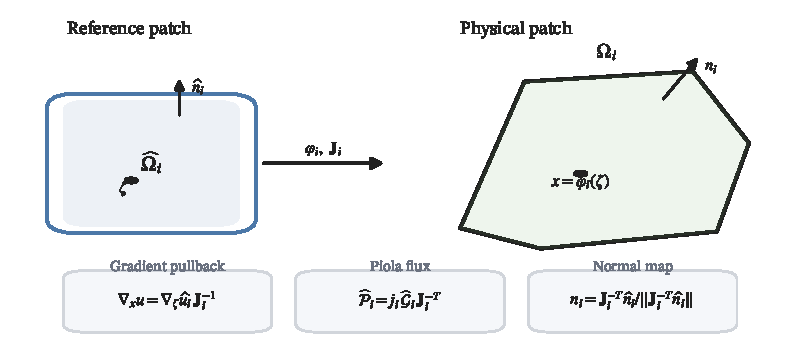
\includegraphics[width=0.98\textwidth]{figures_cmame_core/method/mapped_operator_pub.png}
\caption{Mapped-operator view on one chart. The left side shows the local reference patch, the center arrow represents the chart map and its Jacobian, and the right side shows the corresponding physical patch. The formula cards highlight the three identities the implementation uses directly: gradient pullback, Piola-transformed flux, and normal mapping.}
\label{fig:mapped_operator_schematic}
\end{figure}

\subsection{Special-case global map training for simply connected domains}
\label{sec:global_map_training}
Some examples in the codebase use a single global map
\begin{equation}
\Psi_\theta:B^3\rightarrow \Omega,
\qquad
B^3=\{\boldsymbol{\xi}\in\mathbb{R}^3:\|\boldsymbol{\xi}\|<1\},
\label{eq:global_map}
\end{equation}
instead of a fixed atlas. This special case is used only for simply connected domains where a single volumetric map is feasible. In the validated benchmark set, the ellipsoid uses an analytic global map. The rabbit, Bunny, and torus benchmarks do not use this global-map training stage.

When $\Psi_\theta$ is learned, the implementation combines a positive-determinant barrier, boundary-fidelity terms, and coefficient-regularity terms. A compact way to write the training objective is
\begin{equation}
\mathcal{L}_{\mathrm{map}}
=
\alpha_{\mathrm{bij}}\mathcal{L}_{\mathrm{bij}}
+
\alpha_{\mathrm{geom}}\mathcal{L}_{\mathrm{geom}}
+
\alpha_{\mathrm{coeff}}\mathcal{L}_{\mathrm{coeff}},
\label{eq:global_map_loss}
\end{equation}
where $\mathcal{L}_{\mathrm{bij}}$ penalizes small or negative Jacobian determinant, $\mathcal{L}_{\mathrm{geom}}$ keeps the boundary on the target geometry and the interior inside the domain, and $\mathcal{L}_{\mathrm{coeff}}$ regularizes the mapped operator coefficients induced by the chart Jacobian. In the code this loss is specialized further into bijectivity, ellipticity, isotropy, smoothness, and boundary terms.

\begin{algorithm}[htbp]
\caption{Special-case training of a learned global volumetric map}
\label{alg:global_map_training}
\small
\begin{algorithmic}[1]
\Statex \textbf{Inputs:} reference ball $B^3$; target-domain surface and interior samples; initial map parameters $\theta$;
\StateX optimizer $\mathcal{O}$ with learning-rate schedule $\eta_{\mathrm{map}}^{(t)}$; loss weights $\alpha_{\mathrm{bij}},\alpha_{\mathrm{geom}},\alpha_{\mathrm{coeff}}$; epoch budget $T_{\mathrm{map}}$
\Statex \textbf{Output:} best checkpoint map $\Psi_\theta:B^3\rightarrow\Omega$ satisfying determinant and boundary checks on validation samples
\For{$t=1,\dots,T_{\mathrm{map}}$}
    \State Sample interior points $\boldsymbol{\xi}^{\mathrm{int}}\subset B^3$ and boundary points $\boldsymbol{\xi}^{\partial}\subset \partial B^3$
    \State Evaluate $x^{\mathrm{int}}=\Psi_\theta(\boldsymbol{\xi}^{\mathrm{int}})$, $x^{\partial}=\Psi_\theta(\boldsymbol{\xi}^{\partial})$, and $\mathbf{J}=D_{\boldsymbol{\xi}}\Psi_\theta$
    \State Assemble $\mathcal{L}_{\mathrm{bij}}$, $\mathcal{L}_{\mathrm{geom}}$, and $\mathcal{L}_{\mathrm{coeff}}$ from \eqref{eq:global_map_loss}
    \State Form $\mathcal{L}_{\mathrm{map}}=\alpha_{\mathrm{bij}}\mathcal{L}_{\mathrm{bij}}+\alpha_{\mathrm{geom}}\mathcal{L}_{\mathrm{geom}}+\alpha_{\mathrm{coeff}}\mathcal{L}_{\mathrm{coeff}}$
    \State Compute the mapping-loss gradient $g_{\theta}^{(t)}=\nabla_{\theta}\mathcal{L}_{\mathrm{map}}(\theta^{(t)})$
    \State Update the parameters with the chosen optimizer:
    \Statex \hspace{\algorithmicindent}$\theta^{(t+1)} \leftarrow \mathrm{Update}_{\mathcal{O}}\!\left(\theta^{(t)},g_{\theta}^{(t)};\eta_{\mathrm{map}}^{(t)}\right)$
    \State Record $\min_{\boldsymbol{\xi}}\det \mathbf{J}(\boldsymbol{\xi})$, boundary mismatch, and coefficient diagnostics for checkpointing
    \State Keep the best checkpoint that preserves positive determinant and acceptable boundary fidelity on the validation batch
\EndFor
\State \Return the selected global map $\Psi_\theta$
\end{algorithmic}
\end{algorithm}

Algorithm~\ref{alg:global_map_training} records the training pattern used by the special global-map pipeline. The ellipsoid verification case uses the same mapped-PDE machinery afterward, but its global map is analytic rather than learned.

\subsection{Schwarz alternating PINN on a fixed atlas}
\label{sec:schwarz_pinn}
Once a fixed atlas has been constructed, it also determines the natural domain decomposition for the solver. Each chart supplies one local problem, each overlap $\Omega_{ij}$ supplies an artificial interface, and each transition map $\psi_{ij}$ tells us how to compare neighboring chart fields in compatible coordinates \citep{quarteroni1999domain}. For coordinate-chart PINNs this pairing is particularly natural: local residual minimization already takes place on simple reference patches, while the atlas overlap graph $G_{\mathcal A}$ records exactly which neighbors must exchange temporary traces. Relative to a monolithic global PINN, this localizes approximation, conditioning, and sampling; relative to classical Schwarz, each local subproblem is minimized only approximately by gradient-based updates rather than solved exactly.

Let
\begin{equation}
\widehat{u}_i(\cdot;\theta_i):\widehat{\Omega}_i\rightarrow \mathbb{R}^{q}
\label{eq:local_network}
\end{equation}
be the state network on chart $i$, and define the local physical representation
\begin{equation}
u_i(x;\theta_i):=\widehat{u}_i(\pi_i(x);\theta_i),
\qquad x\in\Omega_i.
\label{eq:local_physical_field}
\end{equation}
For overlaps, the artificial Schwarz boundary of chart $i$ is
\begin{equation}
\Gamma_i:=\partial\Omega_i\setminus \partial\Omega,
\qquad
\Gamma_{ij}:=\Gamma_i\cap \Omega_j,
\qquad
\mathcal{N}(i):=\{j\neq i:\Gamma_{ij}\neq\emptyset\}.
\label{eq:schwarz_sets}
\end{equation}
In reference coordinates, the corresponding sets are $\widehat{\Gamma}_{ij}:=\pi_i(\Gamma_{ij})\subset\widehat{\Omega}_i$ and $\widehat{\Gamma}_{i,\partial\Omega}:=\pi_i(\partial\Omega\cap\partial\Omega_i)$, which are the domains on which interface and physical-boundary penalties are sampled in the loss below. The sets $\Gamma_{ij}$ play the same conceptual role as Schwarz interfaces in classical overlapping domain decomposition: they are not physical boundaries of the PDE, but the internal regions where chart-local solutions must agree strongly enough to define a coherent global field. In the chart setting the same overlap also provides the transition map $\psi_{ij}$ needed to compare chart-local predictions in compatible coordinates. In the rabbit implementation, interface samples are drawn from points whose stored atlas membership includes both charts, and the rigid local coordinates \eqref{eq:atlas_rigid_local_coords} are evaluated in both neighboring frames before the chart-to-chart penalties are formed.

In the continuous Schwarz method one would impose Dirichlet, Neumann, or Robin data on these artificial interfaces and solve each local problem to completion before moving to the next subdomain. The released rabbit solver uses a PINN-compatible relaxation of this idea. Neighbor networks are frozen while chart $i$ is updated, and compatibility is enforced by sampled penalties on the overlap rather than by exact boundary imposition. Writing $\theta_j^{(k,\mathrm{fr})}$ for the frozen neighbor state available during sweep $k$, the interface-value term is
\emph{sampled from the neighboring local field $u_j$ itself, not from the global blended field $u_h$}. This point is important for reproducibility: Schwarz transmission in the released solver is chart-to-chart, with the global blend reserved for diagnostics and post-processing after a sweep has been proposed.
\begin{equation}
\mathcal{J}_{i,\mathrm{iv}}^{(k)}
=
\sum_{j\in \mathcal{N}(i)}
\mathbb{E}_{\boldsymbol{\zeta}\sim \widehat{\Gamma}_{ij}}
\left[
\left|
\widehat{u}_i(\boldsymbol{\zeta};\theta_i)
-
\widehat{u}_j\!\left(\psi_{ij}(\boldsymbol{\zeta});\theta_j^{(k,\mathrm{fr})}\right)
\right|^2
\right].
\label{eq:schwarz_iv_loss}
\end{equation}
For scalar Poisson problems the default validated configuration also penalizes projected normal-flux mismatch. Let $n_{ij}(\boldsymbol{\zeta})$ denote the outward unit normal of $\partial\Omega_i$ at the physical point $\varphi_i(\boldsymbol{\zeta})$, restricted to the interface $\Gamma_{ij}$. Define
\begin{equation}
q_i(\boldsymbol{\zeta};\theta_i)
:=
n_{ij}(\boldsymbol{\zeta})\cdot
\nabla_x u_i\!\left(\varphi_i(\boldsymbol{\zeta});\theta_i\right),
\label{eq:schwarz_flux_trace}
\end{equation}
and
\begin{equation}
\mathcal{J}_{i,\mathrm{if}}^{(k)}
=
\sum_{j\in \mathcal{N}(i)}
\mathbb{E}_{\boldsymbol{\zeta}\sim \widehat{\Gamma}_{ij}}
\left[
\left|
q_i(\boldsymbol{\zeta};\theta_i)
-
q_j\!\left(\psi_{ij}(\boldsymbol{\zeta});\theta_j^{(k,\mathrm{fr})}\right)
\right|^2
\right].
\label{eq:schwarz_if_loss}
\end{equation}
The released solver also exposes a Robin-style variant,
\begin{equation}
\mathcal{J}_{i,\mathrm{rb}}^{(k)}
=
\sum_{j\in \mathcal{N}(i)}
\mathbb{E}_{\boldsymbol{\zeta}\sim \widehat{\Gamma}_{ij}}
\left[
\left|
\lambda_R
\left(
\widehat{u}_i(\boldsymbol{\zeta};\theta_i)
-
\widehat{u}_j\!\left(\psi_{ij}(\boldsymbol{\zeta});\theta_j^{(k,\mathrm{fr})}\right)
\right)
+
q_i(\boldsymbol{\zeta};\theta_i)
-
q_j\!\left(\psi_{ij}(\boldsymbol{\zeta});\theta_j^{(k,\mathrm{fr})}\right)
\right|^2
\right],
\label{eq:schwarz_robin_loss}
\end{equation}
but the validated rabbit benchmark uses the penalty form \eqref{eq:schwarz_iv_loss}--\eqref{eq:schwarz_if_loss} rather than the Robin option. In volumetric-atlas mode the code can further add an overlap-interior value penalty on sampled points from $\widehat{\Omega}_{ij}$; despite the legacy variable name \texttt{overlap\_h1}, the current implementation penalizes value mismatch over the sampled overlap volume rather than the full $H^1$ seminorm.

At Schwarz sweep $k$, the local chart objective is therefore
\begin{align}
\mathcal{J}_i^{(k)}(\theta_i;\eta)
=&
\lambda_{\mathrm{pde}}\,
\mathbb{E}_{\boldsymbol{\zeta}\sim \widehat{\Omega}_i}\!\left[\|\widehat{\mathcal{R}}_i(\boldsymbol{\zeta};\theta_i,\eta)\|_2^2\right]
+
\lambda_{\mathrm{bc}}\,
\mathbb{E}_{\boldsymbol{\zeta}\sim \widehat{\Gamma}_{i,\partial\Omega}}\!\left[\|\widehat{\mathcal{B}}_i(\boldsymbol{\zeta};\theta_i,\eta)\|_2^2\right]
\nonumber\\
&+
\lambda_{\mathrm{iv}}\,\mathcal{J}_{i,\mathrm{iv}}^{(k)}
+
\lambda_{\mathrm{if}}\,\widetilde{\mathcal{J}}_{i,\mathrm{if}}^{(k)}
+
\lambda_{\mathrm{ov}}\,\mathcal{J}_{i,\mathrm{ov}}^{(k)}
+
\lambda_{\mathrm{data}}\,\mathcal{J}_{i,\mathrm{data}}(\theta_i,\eta),
\label{eq:schwarz_local_loss}
\end{align}
where $\widetilde{\mathcal{J}}_{i,\mathrm{if}}^{(k)}$ denotes either the projected-flux penalty \eqref{eq:schwarz_if_loss} or the Robin residual \eqref{eq:schwarz_robin_loss}, and $\mathcal{J}_{i,\mathrm{ov}}^{(k)}$ denotes the optional volumetric overlap penalty. The practical default is the projected-flux penalty with frozen-neighbor traces. This distinction matters: the present solver is Schwarz-inspired in its transmission logic, but each chart update is still carried out by optimizer steps on a neural loss, not by an exact local PDE solve.

One sweep of the atlas solver can be written abstractly as
\begin{equation}
\Theta^{(k+1)}=\mathfrak{S}\!\left(\Theta^{(k)};\eta\right),
\qquad
\Theta^{(k)}:=(\theta_1^{(k)},\dots,\theta_M^{(k)}),
\label{eq:schwarz_sweep}
\end{equation}
where $\mathfrak{S}$ denotes one multiplicative Schwarz pass over the chart set. In the validated rabbit solver this sweep is multiplicative at the level of overlapping neighbors: later charts in the sweep see the most recent accepted states of earlier charts, while non-overlapping charts may be grouped into the same graph color and updated concurrently on compatible accelerator backends without violating the frozen-neighbor assumption on overlap pairs. This is why the released implementation is best described as a multiplicative Schwarz method with limited within-color parallelism, not as a fully additive update.
The color groups used in Algorithm~\ref{alg:atlas_sapinn_training} are derived from a graph-coloring of the chart-overlap adjacency matrix: two charts may share a color only if they do not overlap, which makes within-color updates independent for the purposes of the frozen-neighbor Schwarz step.

After an accepted sweep, the global blended field is
\begin{equation}
u_h^{(k)}(x)=\sum_{i=1}^{M}\omega_i(x)\,u_i(x;\theta_i^{(k)}).
\label{eq:schwarz_global_field}
\end{equation}

\begin{figure}[htbp]
\centering
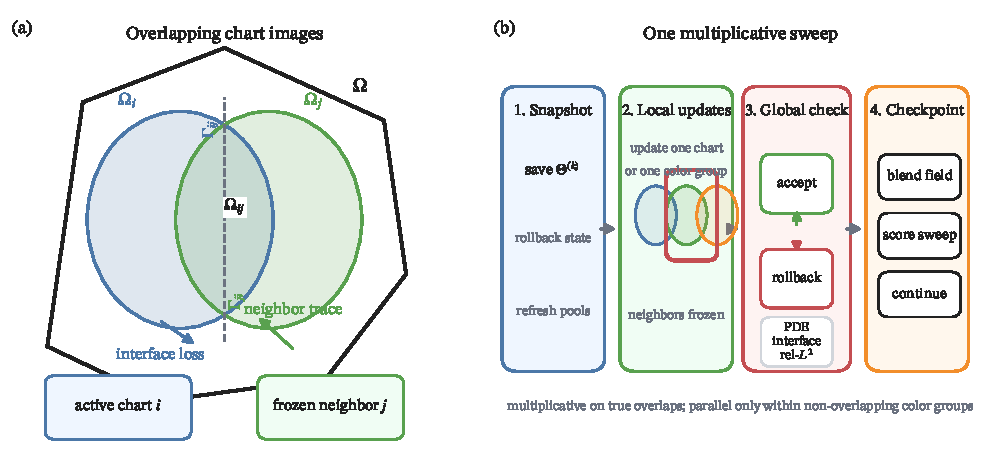
\includegraphics[width=0.98\textwidth]{figures_cmame_core/method/schwarz_schematic_pub.png}
\caption{Conceptual and algorithmic view of fixed-atlas SA-PINN coupling. Panel (a) shows two overlapping chart images inside the physical body. The overlap $\Omega_{ij}$ induces the artificial interfaces $\Gamma_{ij}$ and $\Gamma_{ji}$ on which neighboring chart solutions exchange temporary transmission data during training. Panel (b) shows one multiplicative Schwarz sweep as implemented in the rabbit solver: the code snapshots the full chart state, updates one active chart or non-overlapping color group while neighbor states are detached, evaluates global residual and interface diagnostics, and then accepts the whole sweep or restores the previous state.}
\label{fig:schwarz_schematic}
\end{figure}

\begin{algorithm}[htbp]
\caption{Fixed-atlas SA-PINN training by multiplicative Schwarz sweeps}
\label{alg:atlas_sapinn_training}
\small
\begin{algorithmic}[1]
\Statex \textbf{Inputs:} validated atlas $\mathcal{A}$; chart-local networks $\{\widehat{u}_i(\cdot;\theta_i)\}_{i=1}^M$;
\StateX optional global parameters $\eta$; local optimizers; sweep budget $K$; local-step budget $N_{\mathrm{loc}}$
\Statex \textbf{Outputs:} selected checkpoint $\{\theta_i\}_{i=1}^M$ and blended field $u_h$
\Statex \textit{Initialization}
\State Initialize chart parameters $\theta_i$ and any trainable global parameters $\eta$
\State Evaluate the initial blended field and initialize checkpoint metrics
\For{$k=0,\dots,K-1$}
    \Statex \textit{Pre-sweep setup}
    \State Store a snapshot of the full chart state $\Theta^{(k)}$
    \State Refresh sweep-level sampling pools and effective interface weights
        \For{each color group $g$ from the graph-coloring of the chart-overlap adjacency matrix}
        \Statex \textit{Local chart updates}
        \For{each active chart $i\in g$ sequentially, or concurrently when charts in $g$ do not overlap}
            \For{$n=1,\dots,N_{\mathrm{loc}}$}
                \State Sample PDE, physical-boundary, interface, and optional supervision points on chart $i$
                \State Query neighbors only through frozen predictions on sampled overlap points
                \State Assemble the local loss $\mathcal{J}_i^{(k)}$ in \eqref{eq:schwarz_local_loss}
                \State Update $\theta_i$ while all neighbor contributions remain detached
            \EndFor
        \EndFor
    \EndFor
    \Statex \textit{Global acceptance test}
    \State Form the proposed blended field by \eqref{eq:schwarz_global_field}
    \State Evaluate global PDE, boundary, interface, and relative-$L^2$ diagnostics
    \If{the sweep violates the trust-region admissibility test}
        \State Restore the pre-sweep snapshot $\Theta^{(k)}$ and reduce the learning rate
    \Else
        \State Accept the sweep and refresh checkpoint statistics
        \State Update adaptive weights if enabled
    \EndIf
\EndFor
\State \Return the selected checkpoint and its blended field $u_h$
\end{algorithmic}
\end{algorithm}

Algorithm~\ref{alg:atlas_sapinn_training} records the core training loop behind the fixed-atlas rabbit Poisson benchmark. The accepted state is decided at the sweep level rather than chart by chart, and any parallelism is restricted to non-overlapping color groups, so the released solver still behaves as a multiplicative Schwarz method on every true overlap pair.



\section{Implementation}
\label{sec:implementation}

This section records how the methodology of Section~\ref{sec:methodology} is realized in code. The goal is not to catalogue the entire repository, but to document the implementation choices that materially affect robustness, reproducibility, and interpretation of the validated benchmarks. Workflow transparency and backend-specific execution metadata are reported in Appendix~\ref{sec:appendix_impl_details}.

\subsection{Software stack and numerical separation of responsibilities}
\label{sec:impl_stack}

All neural networks are implemented in PyTorch \citep{paszke2019pytorch}. Automatic differentiation is used both for PDE residuals and for the Jacobians needed by the chart maps and constitutive models. Jacobian inversion is carried out in the forward pass with \texttt{torch.linalg.inv}, while condition diagnostics are evaluated under \texttt{torch.no\_grad()} to avoid unnecessary instability near nearly singular samples. The framework is implemented in a hardware-agnostic PyTorch environment capable of acceleration on Metal, CUDA, and CPU backends, and the validated runs reported here were executed through the same code path used for development.

A guiding implementation principle is the separation of geometry from PDE solving. Geometry processing produces an SDF, a volumetric atlas, and a decoder/mask representation that are frozen before the field solver is trained. This separation is what makes the numerical evidence interpretable: if a benchmark fails after the geometry gate has passed, the failure can be attributed to the PDE solver or the coupling logic rather than to a moving geometry target.

Supporting geometry utilities use \texttt{open3d}, \texttt{pysdf}, \texttt{mesh\_to\_sdf}, and \texttt{trimesh}; post-processing uses VTK through \texttt{pyvista} and ParaView. These libraries matter for reproducibility because the entire atlas pipeline depends on reliable signed-distance queries, surface repair, and consistent volumetric export.

\subsection{Neural network architectures}
\label{sec:impl_architectures}

The implementation uses several neural-network families, but only a subset of them is central to the main-text claims. Table~\ref{tab:impl_networks} therefore focuses on the architectures that directly support the validated examples: the global SDF used in the Bunny geometry benchmark, the special-case global map used on simply connected geometry, the decoder-mask pair that realizes the rabbit atlas, and the chart-local field networks used by the rabbit Poisson solver. Supporting prototypes remain in the repository, but they are omitted from the table so that the main paper stays focused on scientifically consequential design choices rather than on an exhaustive architecture catalog.

\begin{table}[htbp]
\centering
\scriptsize
\setlength{\tabcolsep}{1.8pt}
\renewcommand{\arraystretch}{1.03}
\begin{threeparttable}
\caption{Neural-network families used in the implementation section. Configurations are quoted directly from source code class definitions and, where available, canonical checkpoint metadata. When a checkpoint records only a top-level architecture label, the table reports the constructor configuration instantiated by the corresponding solver path.}
\label{tab:impl_networks}
\begin{tabular}{>{\raggedright\arraybackslash}p{1.8cm}>{\raggedright\arraybackslash}p{2.05cm}>{\raggedright\arraybackslash}p{1.55cm}>{\raggedright\arraybackslash}p{6.1cm}>{\raggedright\arraybackslash}p{1.3cm}}
\toprule
Code name / symbol & Purpose & Type & Exact configuration & Reference \\
\midrule
\texttt{SDFNet} & global volumetric level-set for inside/outside queries and atlas construction & \shortstack[l]{fully connected\\ \texttt{tanh} MLP} & \shortstack[l]{$3\!\rightarrow\!1$; width $128$, depth $6$;\\ Xavier initialization; Bunny checkpoint stores\\ \texttt{model\_kwargs=\{width:128, depth:6\}}} & This work \\
\texttt{MappingNet} & special-case ball-to-domain map & \shortstack[l]{residual chart map\\ on \texttt{tanh} MLP} & \shortstack[l]{$3\!\rightarrow\!3$; width $128$, depth $6$;\\ learned \texttt{log\_scale}, \texttt{shift}, \texttt{raw\_disp};\\ displacement cap \texttt{disp\_cap}=0.45} & This work \\
\texttt{ChartDecoder} & differentiable chart map & \shortstack[l]{fully connected\\ \texttt{tanh} MLP with\\ residual correction} & \shortstack[l]{$3\!\rightarrow\!3$; width $64$, depth $4$;\\ \texttt{raw\_scale} initialized to $-1.8$; residual amplitude\\ $0.20\,\tanh(\texttt{raw\_scale})\,r_i$; checkpoint stores\\ width $64$, depth $4$} & This work \\
\texttt{MaskNet} & chart-validity logits and PoU weights & \shortstack[l]{fully connected\\ \texttt{tanh} MLP} & \shortstack[l]{$3\!\rightarrow\!1$; width $48$, depth $3$;\\ checkpoint stores width $48$, depth $3$} & This work \\
\shortstack[l]{\texttt{LocalPoissonPINN}\\ (\texttt{mlp})} & dense chart-local scalar field solve & \shortstack[l]{fully connected\\ \texttt{tanh} PINN} & \shortstack[l]{$3\!\rightarrow\!1$; width $64$, depth $4$;\\ \texttt{attempt19\_w4} records \texttt{arch=mlp},\\ residual scale $0.1$, \texttt{residual\_zero\_init=True}} & \shortstack[l]{PINN \citep{raissi2019physicsinformed};\\ this work} \\
\shortstack[l]{\texttt{Compact}\\ \texttt{ChartNet}} & localized chart-local field solve & \shortstack[l]{mixture of small\\ \texttt{tanh} MLPs\\ + softmax PoU} & \shortstack[l]{9 subnets; each width $32$, depth $2$;\\ \texttt{tau\_scale}=0.125; checkpoint stores \texttt{arch=compact};\\ exact subnetwork values come from the solver path} & This work \\
\bottomrule
\end{tabular}
\begin{tablenotes}[flushleft]
\item Configurations come from the source definitions and canonical checkpoints cited in the text.
\end{tablenotes}
\end{threeparttable}
\end{table}

\subsubsection{Implicit geometry and mapping networks}
The geometry stage is built on fully connected \texttt{tanh} MLPs with Xavier initialization, but the roles of those networks are distinct. The canonical Bunny trainer uses \texttt{SDFNet}, a $3\!\rightarrow\!1$ network with width $128$ and depth $6$, to learn the volumetric level-set field required for inside/outside queries and later chart placement. The special-case global-map path uses \texttt{MappingNet}, which keeps the same $128\times 6$ backbone but augments it with learned scale, translation, and capped displacement parameters. For that reason, the manuscript treats the ball-to-domain map as a practical geometric prior rather than as a bijection by construction.

The training design of the geometry networks is deliberately simple in the canonical Bunny pipeline. The released global SDF trainer uses a static weighted sum in \eqref{eq:impl_sdf_loss}, optimized with Adam and parser defaults $w_{\mathrm{surf}}=10$, $w_{\mathrm{eik}}=1$, $w_{\mathrm{norm}}=1$, and $w_{\mathrm{sign}}=2$. It does not use GradNorm, PCGrad, or any other explicit gradient-conflict mitigation. Supporting chartwise SDF prototypes remain in the repository, but they are not central to the main-text claims and are therefore omitted from the table.

\subsubsection{Differentiable atlas realization networks}
Once a volumetric prior is available, the atlas is realized by a paired decoder-mask architecture. Each \texttt{ChartDecoder} is a $3\!\rightarrow\!3$ \texttt{tanh} MLP with width $64$ and depth $4$. It refines a rigid seed-based local frame by adding a learned residual scaled by $0.20\,\tanh(\texttt{raw\_scale})\,r_i$ rather than learning the chart from scratch. Each chart is paired with a smaller \texttt{MaskNet}, a $3\!\rightarrow\!1$ \texttt{tanh} MLP with width $48$ and depth $3$, whose job is to generate stable validity logits and partition-of-unity weights rather than to reproduce geometry.

In the canonical rabbit workflow, these decoder and mask networks are trained once during the atlas stage and then frozen before PDE training begins. The canonical atlas checkpoint records those widths and depths directly, and the same checkpoint is screened by coverage, overlap-consistency, and foldover gates before any chart-local field solve is attempted. That gate-controlled freeze is the key scientific reason for reporting these architectures in the main text.

\subsubsection{Chart-local field solvers}
The rabbit Poisson solver exposes a dense baseline and a localized compact alternative. The dense baseline, \texttt{LocalPoissonPINN} with \texttt{arch="mlp"}, is a $3\!\rightarrow\!1$ \texttt{tanh} network with width $64$ and depth $4$; the tradeoff checkpoint \texttt{attempt19\_w4} records exactly that configuration. The flagship rabbit run instead uses \texttt{CompactChartNet}, which replaces one monolithic chart network by a small sub-atlas inside each chart: $9$ sub-seeds, one $32\times 2$ \texttt{tanh} subnet per sub-seed, and a softmax partition of unity with $\tau=0.125\,r_i$. This design localizes approximation power within each chart and is the main architectural reason the compact run achieves smoother Schwarz histories than the dense baseline.

The same frozen atlas can also host a non-neural local discretization: the repository now includes a rabbit chart-local P1 FEM variant that reuses the decoder, mask, overlap graph, and Schwarz infrastructure of the PINN solver. Because that variant is not a neural architecture, it is discussed in Example~2 rather than catalogued in the network table.

The solver classes should be distinguished from the stabilization logic wrapped around them. PCGrad, trust-region rejection, and staged loss-weight schedules are implemented in the Schwarz training routine rather than in the network definitions themselves. The torus inverse benchmark is more different still: it does not train a neural field over the body, but only the global scalars \texttt{mu\_raw} and \texttt{K\_raw} under fixed soft chart weights. That is why Example~4 should be read as a controlled parameter-identification benchmark rather than as another chart-local neural-field solve.

\subsection{Geometry pipeline and rigid quality assurance}
\label{sec:impl_pipeline}

The geometry stage is executed as a four-step pipeline. The point of spelling it out here is not merely procedural. Each stage constructs a mathematical object that the downstream solver actually needs: a volumetric level-set model for point-in-domain queries, a coarse chart layout, a learned realization of the chart maps and overlap weights, and finally a set of gate metrics that determine whether the atlas is admissible for PDE training. This is the main difference from a purely surface-reconstruction pipeline. It is not enough for the learned representation to pass near the observed surface; it must also provide a volumetric interior, support local chart coordinates, and remain stable under pullback of the PDE operator.

\paragraph{Stage 1: volumetric signed-distance modeling.}
For imported geometry, let $X_{\partial}=\{(x_k,n_k)\}_{k=1}^{N}$ denote the observed surface samples together with their oriented normals. The first requirement is then a scalar level-set model
\begin{equation}
s_{\vartheta}:\mathbb{R}^3\rightarrow \mathbb{R},
\qquad
\Omega \approx \{x\in\mathbb{R}^3:s_{\vartheta}(x)<0\},
\qquad
\partial\Omega \approx \{x\in\mathbb{R}^3:s_{\vartheta}(x)=0\},
\label{eq:impl_sdf_levelset}
\end{equation}
so that inside/outside classification, near-surface sampling, and volumetric chart seeding can all be defined without a tetrahedral mesh. In the released code this object is represented by the global SDF architecture summarized in Section~\ref{sec:impl_architectures} and trained on surface points $X_{\partial}$ with outward normals $N_{\partial}$. The training loss is
\begin{align}
\mathcal{L}_{\mathrm{SDF}}
=&
\lambda_{\mathrm{surf}}\,
\mathbb{E}_{x\sim X_{\partial}}\!\left[|s_{\vartheta}(x)|\right]
+
\lambda_{\mathrm{norm}}\,
\mathbb{E}_{(x,n)\sim (X_{\partial},N_{\partial})}
\left[
1-\frac{\nabla s_{\vartheta}(x)}{\|\nabla s_{\vartheta}(x)\|_2}\cdot n
\right]
\nonumber\\
&+
\lambda_{\mathrm{eik}}\,
\mathbb{E}_{x\sim B}
\left[
\big(\|\nabla s_{\vartheta}(x)\|_2-1\big)^2
\right]
+
\lambda_{\mathrm{sign}}\,
\mathcal{L}_{\mathrm{sign}},
\label{eq:impl_sdf_loss}
\end{align}
with sign supervision
\begin{align}
\mathcal{L}_{\mathrm{sign}}
=&
\tfrac12\,
\mathbb{E}_{(x,n)\sim (X_{\partial},N_{\partial})}
\left[
\operatorname{softplus}\!\big(s_{\vartheta}(x-\delta n)\big)
+
\operatorname{softplus}\!\big(-s_{\vartheta}(x+\delta n)\big)
\right]
\nonumber\\
&+
\tfrac12\,
\mathbb{E}_{x\sim B_{\mathrm{far}}}
\left[
\operatorname{softplus}\!\big(-s_{\vartheta}(x)\big)
\right].
\label{eq:impl_sdf_sign}
\end{align}
Equation~\eqref{eq:impl_sdf_levelset} is the mathematical requirement behind the Bunny example: without a usable volumetric level-set, the later atlas construction has no reliable way to place seeds in the interior or to reject decoder outputs that leave the body. The sign-anchor term in \eqref{eq:impl_sdf_sign} is the most delicate on thin-featured geometry because a single offset $\delta$ that works in the bulk may cross the surface in narrow regions such as the Stanford Bunny ears. In that sense, the SDF is not a cosmetic preprocessing step; it is the volumetric prior that turns surface observations into a usable interior geometry model.

\paragraph{Stage 2: atlas construction.}
Once a stable $s_{\vartheta}$ is available, the domain is covered by $M$ overlapping volumetric charts. In the implementation this stage requires a seed set $\{c_i\}_{i=1}^{M}$ (denoted $s_i$ in the methodology of Section~\ref{sec:atlas_geometry}), local frames $Q_i=[t_{1,i}\;t_{2,i}\;n_i]\in\mathbb{R}^{3\times 3}$, and support radii $\{r_i\}_{i=1}^{M}$. For any physical point $x$, the chart-local coordinates are initialized by
\begin{equation}
\boldsymbol{\zeta}_i(x)
=
\begin{bmatrix}
(x-c_i)\cdot t_{1,i}\\
(x-c_i)\cdot t_{2,i}\\
(x-c_i)\cdot n_i
\end{bmatrix},
\label{eq:impl_local_coords}
\end{equation}
and the coarse overlap membership is chosen from the seed distances
\begin{equation}
d_i(x)=\|x-c_i\|_2,
\qquad
\chi_i(x)=\mathbf{1}\!\left\{
d_i(x)\le (1+\alpha)\min_{j} d_j(x)
\right\},
\label{eq:impl_membership}
\end{equation}
where $\alpha$ is tuned so that the empirical overlap fraction matches the target overlap. In the volumetric atlas builder, candidate seeds are accepted only when $s_{\vartheta}(c_i)<0$, so the SDF from Stage~1 is already part of the chart-construction logic. This stage therefore does more than scatter points in space: it defines the local coordinate frames and coarse support sets on which the learned chart maps will later operate. Relative to a surface-only atlas, the extra requirement is that the seeds and supports must be meaningful in the interior of the body, not only on the observed boundary.

\paragraph{Stage 3: decoder and mask training.}
The coarse atlas is then promoted into a differentiable atlas by learning a decoder $\Phi_i$ and a mask logit $\ell_i$ for each chart. In implementation terms, the abstract chart map $\varphi_i$ from Section~\ref{sec:methodology} is realized by
\begin{align}
\Phi_i(\boldsymbol{\zeta})
=&
\;c_i
+
\zeta_1 t_{1,i}
+
\zeta_2 t_{2,i}
+
\zeta_3 n_i
+
a_i r_i\,\mathcal{N}_i(\boldsymbol{\zeta}/r_i),
\label{eq:impl_decoder_map}\\
\ell_i(\boldsymbol{\zeta})
=&
\;M_i(\boldsymbol{\zeta}/r_i),
\qquad
p_i(x)=\sigma\!\big(\ell_i(\boldsymbol{\zeta}_i(x))\big),
\qquad
\omega_i(x)=\frac{\exp(\ell_i(\boldsymbol{\zeta}_i(x)))}{\sum_j \exp(\ell_j(\boldsymbol{\zeta}_j(x)))},
\label{eq:impl_mask_weights}
\end{align}
where $\mathcal{N}_i$ and $M_i$ denote the decoder and mask networks summarized in Section~\ref{sec:impl_architectures}, and $a_i$ is a learned residual amplitude. The decoder loss used in the code is a weighted combination
\begin{equation}
\mathcal{L}_{\mathrm{atlas}}
=
\lambda_{\mathrm{rec/dom}}\mathcal{L}_{\mathrm{rec/dom}}
+
\lambda_{\mathrm{mask}}\mathcal{L}_{\mathrm{mask}}
+
\lambda_{\mathrm{ov}}\mathcal{L}_{\mathrm{ov}}
+
\lambda_{\mathrm{jac}}\mathcal{L}_{\mathrm{jac}}
+
\lambda_{\mathrm{cov}}\mathcal{L}_{\mathrm{cov}},
\label{eq:impl_atlas_total}
\end{equation}
with the component terms matching the released training script:
\begin{align}
\mathcal{L}_{\mathrm{rec}}
=&
\sum_{i=1}^{M}
\mathbb{E}_{x\in X_i^{+}}
\left[
\|\Phi_i(\boldsymbol{\zeta}_i(x))-x\|_2^2
\right],
\label{eq:impl_atlas_recon}\\
\mathcal{L}_{\mathrm{dom}}
=&
\sum_{i=1}^{M}
\mathbb{E}_{\boldsymbol{\zeta}\sim [-r_i,r_i]^3}
\left[
\operatorname{ReLU}\!\big(s_{\vartheta}(\Phi_i(\boldsymbol{\zeta}))-\tau_{\mathrm{sdf}}\big)^2
\right],
\label{eq:impl_atlas_domain}\\
\mathcal{L}_{\mathrm{mask}}
=&
\sum_{i=1}^{M}
\mathbb{E}_{x\in X_i^{+}}
\left[
\operatorname{softplus}\!\big(-\ell_i(\boldsymbol{\zeta}_i(x))\big)
\right]
+
\sum_{i=1}^{M}
\mathbb{E}_{x\in X_i^{-}}
\left[
\operatorname{softplus}\!\big(\ell_i(\boldsymbol{\zeta}_i(x))\big)
\right],
\label{eq:impl_atlas_mask}\\
\mathcal{L}_{\mathrm{ov}}
=&
\sum_{i<j}
\mathbb{E}_{x\in X_{ij}}
\left[
\|\Phi_i(\boldsymbol{\zeta}_i(x))-\Phi_j(\boldsymbol{\zeta}_j(x))\|_2^2
\right],
\label{eq:impl_atlas_overlap}\\
\mathcal{L}_{\mathrm{jac}}
=&
\sum_{i=1}^{M}
\mathbb{E}_{\boldsymbol{\zeta}\sim \widehat{\Omega}_i}
\left[
\operatorname{softplus}\!\big(\delta_{\det}-\det D\Phi_i(\boldsymbol{\zeta})\big)^2
\right],
\label{eq:impl_atlas_jac}\\
\mathcal{L}_{\mathrm{cov}}
=&
\mathbb{E}_{x\sim X}
\left[
\operatorname{softplus}\!\big(\tau_{\mathrm{cov}}-\max_i p_i(x)\big)
-\log \omega_{\mathrm{pri}(x)}(x)
\right].
\label{eq:impl_atlas_cov}
\end{align}
Here $X_i^{+}$ and $X_i^{-}$ denote the samples currently labeled inside and outside chart $i$, $X_{ij}$ denotes sampled overlap points shared by charts $i$ and $j$, and $X$ denotes the global point cloud or interior validation set used by the atlas trainer. The threshold $\tau_{\mathrm{sdf}}$ in \eqref{eq:impl_atlas_domain} is the tolerated signed-distance margin used to penalize decoder outputs that leave the admissible interior.
The distinction between $\mathcal{L}_{\mathrm{rec}}$ and $\mathcal{L}_{\mathrm{dom}}$ matters for interpretation. Surface-based atlas fitting uses \eqref{eq:impl_atlas_recon}, while the volumetric Bunny continuation replaces it by \eqref{eq:impl_atlas_domain}. This is the clearest place where our reconstruction problem departs from the surface-reconstruction template: the goal is not only to fit overlapping boundary patches, but to learn volumetric charts whose decoded images remain inside the body and can later support local PDE solves.

\paragraph{Stage 4: iterative atlas refinement strategy.}
Before any PDE training starts, the atlas must pass explicit geometric gate metrics. In the released training code these are coverage, overlap consistency, and foldover ratio, with an additional boundary RMSE check when a direct pointwise reconstruction target is available. In symbols,
\begin{align}
g_{\mathrm{cov}}
=&
\mathbb{P}_{x\sim X}
\left[
\max_i p_i(x)>\tau_{\mathrm{cov}}
\right],
\nonumber\\
g_{\mathrm{ov}}
=&
\mathbb{E}_{x\in X_{\mathrm{ov}}}
\left[
\|\Phi_i(\boldsymbol{\zeta}_i(x))-\Phi_j(\boldsymbol{\zeta}_j(x))\|_2
\right],
\nonumber\\
g_{\mathrm{fold}}
=&
\frac{1}{N_J}
\sum_{i,\boldsymbol{\zeta}}
\mathbf{1}_{\{\det D\Phi_i(\boldsymbol{\zeta})\le 0\}},
\label{eq:impl_gate_metrics}\\
g_{\mathrm{rmse}}
=&
\left(
\mathbb{E}_{x\sim X}
\left[
\left\|
\sum_{i=1}^{M}\omega_i(x)\Phi_i(\boldsymbol{\zeta}_i(x))-x
\right\|_2^2
\right]
\right)^{1/2}.
\label{eq:impl_gate_rmse}
\end{align}
The atlas is accepted only if these metrics lie inside prescribed admissible bands. If a gate fails, the implementation does not simply bypass the check. Instead, it enters an iterative atlas refinement loop in which chart seeds, support radii, decoder states, and mask parameters are updated so as to reduce the violated metric on the next trial. This makes the gate stage an algorithmic refinement step rather than a manual cleanup step.

This four-stage structure is central to the paper's computational argument. The forward rabbit Poisson example succeeds in part because the geometry stage is fixed, audited, and frozen before the Schwarz solver is allowed to run. Conversely, the Bunny SDF benchmark shows what happens when the level-set model itself is the main source of uncertainty.

\paragraph{Remark on spherical reference domains.}
The released code makes a deliberate use of spherical, or more precisely ball-shaped, reference domains. In the special global-map pipeline the reference body is the unit ball $B^3$ with boundary $S^2$, while in the volumetric atlas builder each local chart is initialized as a ball chart centered at its seed and then refined by a small learned residual. This design should be interpreted as a geometric prior rather than as a proof of injectivity. The numerical advantage is that the reference metric is isotropic and curvature-regular, so the chart coordinates do not introduce an artificial directional bias before any learning takes place; this tends to stabilize sampling, Jacobian conditioning, and support-radius selection. The price is that neither the global sphere-to-domain map nor the family of local ball charts is bijective by construction. Injectivity must therefore be established a posteriori through the determinant barrier, overlap consistency checks, and foldover gates described above. In the present framework, spherical reference domains are used because they provide a stable computational geometry scaffold, while bijectivity is treated as a monitored quality property rather than as an automatic consequence of the parametrization.

\subsection{Local solver schedule, adaptive regularization, and stabilization}
\label{sec:impl_solver}

The chart-local architectures themselves are summarized in Section~\ref{sec:impl_architectures}. The present subsection focuses on how those chart-local models are stabilized once the geometry stage has been frozen. For the compact solver path, the chart-local field is blended by a smooth partition of unity:
\begin{equation}
u_{\mathrm{chart}}(\boldsymbol{\zeta})
=
\sum_{m=0}^{8}\phi_m(\boldsymbol{\zeta})\,u_m(\boldsymbol{\zeta}-\boldsymbol{s}_m),
\qquad
\phi_m(\boldsymbol{\zeta})=\frac{\exp(-\|\boldsymbol{\zeta}-\boldsymbol{s}_m\|^2/2\tau^2)}{\sum_{m'}\exp(-\|\boldsymbol{\zeta}-\boldsymbol{s}_{m'}\|^2/2\tau^2)}.
\label{eq:compact_pou_impl}
\end{equation}
This construction preserves differentiability of the autograd Laplacian while localizing the approximation within each chart.

Two constants are particularly important for robustness: the decoder overlap weight and the CompactChartNet localization scale $\tau_{\mathrm{scale}}$. In the released validated runs these were fixed at problem-specific values, but they are better interpreted as adaptive regularization constants than as magic numbers. A practical overlap-weight heuristic is
\begin{equation}
w_{\mathrm{ov}}^{(n+1)}=
\mathrm{clip}\!\left(
w_{\mathrm{ov}}^{(n)}
\left(\frac{\mathcal{L}_{\mathrm{cov}}^{(n)}}{\mathcal{L}_{\mathrm{ov}}^{(n)}+\varepsilon}\right)^{\beta},
w_{\min},w_{\max}
\right),
\label{eq:adaptive_overlap_weight}
\end{equation}
which increases overlap enforcement only when coverage is already acceptable and the overlap loss is under-resolved. Likewise, a robust continuation for the CompactChartNet bandwidth is
\begin{equation}
\tau_{\mathrm{scale}}^{(n)}
=
\tau_{\max}-\big(\tau_{\max}-\tau_{\min}\big)
\min\!\left(1,\frac{n}{N_{\mathrm{warm}}}\right),
\label{eq:adaptive_tau_schedule}
\end{equation}
so the basis starts wide during warmup and contracts only after the boundary and interface losses have stabilized. The canonical compact rabbit run itself uses the fixed constructor value $\tau_{\mathrm{scale}}=0.125$ recorded in the instantiated solver path, so \eqref{eq:adaptive_tau_schedule} should be read as a robustness-oriented continuation heuristic rather than as a description of the current archived checkpoint.

The released rabbit solver also uses three additional stabilization devices. First, the PDE weight is ramped up gradually so that the Dirichlet and interface terms can settle before the stiff residual dominates. Second, PCGrad \citep{yu2020gradient} is used when the PDE and manufactured-anchor gradients point in conflicting directions. Third, a trust-region filter rejects any local Schwarz update that causes an unacceptable increase in global relative $L^2$ error and reduces the local learning rate after rejection. Together with plateau detection and checkpoint selection, these mechanisms produce the stable 61-iteration rabbit run reported in Section~\ref{sec:example2}.

Finally, the curvature-weighted simplification used in the rabbit Poisson benchmarks is worth stating explicitly. Because the chart frames are initialized to be nearly orthonormal, the implementation can evaluate the Laplacian directly in chart coordinates during the stable phase of training, which regularizes the operator evaluation when the full mapped Jacobian becomes poorly conditioned in high-curvature regions. We treat this choice as a trade-off study rather than as an implementation shortcut. If the local metric distortion satisfies $\|\mathbf{J}_i(\boldsymbol{\zeta})^T\mathbf{J}_i(\boldsymbol{\zeta})-\mathbf{I}\|_2\le \varepsilon_g$ on the admissible collocation set, then the induced perturbation in the mapped diffusion tensor is first-order in $\varepsilon_g$, so the resulting operator error is controlled by the atlas quality gate. In return, the direct chart-coordinate evaluation acts as a regularizer near nearly singular Jacobian samples and is substantially more stable numerically on the validated rabbit benchmark. The manuscript therefore presents this as a curvature-weighted computational simplification with a monitored geometry-induced error budget, not as a universal identity of the method.
\section{Benchmark problems and numerical results}
\label{sec:benchmark_formulations}

\subsection{Reporting protocol and evaluation criteria}
This section asks a narrow question: where does the current atlas-based implementation already provide credible numerical evidence, and what is the scope of the claim supported by that evidence? The codebase now contains a direct rabbit head-to-head between chart-local PINN and chart-local P1 FEM solves posed on the same mapped-operator workflow family, so the evidence can compare neural and classical local discretizations on one frozen geometric scaffold. The emphasis here is therefore on code-faithful reporting of validated artifacts. All numerical values come from archived metric files and checkpoint registries, not from hand-copied terminal output.

We therefore focus on four mature examples that support distinct parts of the paper's argument: analytic verification on the ellipsoid, a fixed-atlas rabbit Poisson solve, a volumetric neural SDF benchmark on the Stanford Bunny PLY, and a controlled torus inverse Neo-Hookean benchmark. For the forward Poisson cases we report relative and absolute $L^2$ errors, maximum pointwise error, and runtime; for the Bunny geometry benchmark we report the surface, normal-alignment, Eikonal, and sign-anchor losses; and for the torus inverse benchmark we report the traction mismatch together with the relative errors in the recovered constitutive parameters.

\begin{table}[htbp]
\centering
\scriptsize
\setlength{\tabcolsep}{2.2pt}
\caption{Traceability map for the main-text examples. The table records the canonical artifact used in each subsection narrative; interpretation and scientific claims are carried by the example discussions themselves.}
\label{tab:benchmark_map}
\begin{tabular}{>{\raggedright\arraybackslash}p{1.9cm}>{\raggedright\arraybackslash}p{1.35cm}>{\raggedright\arraybackslash}p{3.3cm}>{\raggedright\arraybackslash}p{1.95cm}}
\toprule
Case & Scientific role & Primary script & Canonical run \\
\midrule
Ellipsoid Poisson & verification & \shortstack[l]{\texttt{pinn\_3d\_}\\ \texttt{ellipsoid\_}\\ \texttt{mapped\_}\\ \texttt{sphere.py}} & \shortstack[l]{\texttt{ellipsoid\_20260212}\\ \texttt{\_180204}} \\
Rabbit Poisson & \shortstack[l]{field\\ solve} & \shortstack[l]{\texttt{run\_poisson\_}\\ \texttt{rabbit\_atlas\_}\\ \texttt{schwarz.py}} & \shortstack[l]{\texttt{attempt20c}\\ \texttt{\_compact}} \\
\shortstack[l]{Stanford Bunny\\ neural SDF} & \shortstack[l]{geometry\\ stage} & \shortstack[l]{\texttt{train\_sdf\_}\\ \texttt{rabbit.py}} & \shortstack[l]{\texttt{bunny\_sdf}\\ \texttt{\_v3}} \\
\shortstack[l]{Torus inverse\\ (original atlas)} & \shortstack[l]{controlled\\ inverse} & \shortstack[l]{\texttt{run\_torus\_}\\ \texttt{inverse\_neohookean\_}\\ \texttt{atlas.py}} & \shortstack[l]{\texttt{torus\_inverse}\\ \texttt{\_mps\_dense\_v4}} \\
\bottomrule
\end{tabular}
\end{table}

% Example 1 source traceability (comment only; not visible in the compiled PDF).
% Paths below are relative to the PINN_coordinate_chart_3Dgeometry/ project root.
% Code:
%   - src/pinn_3d_ellipsoid_mapped_sphere.py
%     Analytic mapped-Poisson verification script for the ellipsoid benchmark.
% Data / run artifacts:
%   - runs/examples/ellipsoid3d_20260212_180204/
%     Canonical archived run directory used for the reported verification metrics and figure export.
% Notes:
%   - This benchmark has no external raw geometry directory because the ellipsoid map, forcing,
%     and exact solution are generated analytically inside the script.
\subsection{Example 1: forward Poisson on the ellipsoid}
\label{sec:example1}
The common physical problem is
\begin{equation}
-\Delta_x u = f \quad \text{in }\Omega,
\qquad
u=g \quad \text{on }\partial\Omega.
\label{eq:ex1_phys}
\end{equation}
For a chart-local scalar field, the mapped residual is
\begin{equation}
\widehat{\mathcal{R}}^{(1)}_i(\boldsymbol{\zeta})
:=
-\nabla_{\boldsymbol{\zeta}}\cdot\left(
\mathbf{A}_i(\boldsymbol{\zeta})\nabla_{\boldsymbol{\zeta}} \widehat{u}_i(\boldsymbol{\zeta})
\right)
- j_i(\boldsymbol{\zeta})\,f(\varphi_i(\boldsymbol{\zeta})),
\qquad
\mathbf{A}_i(\boldsymbol{\zeta}):=j_i(\boldsymbol{\zeta})\mathbf{J}_i(\boldsymbol{\zeta})^{-1}\mathbf{J}_i(\boldsymbol{\zeta})^{-T}.
\label{eq:ex1_residual}
\end{equation}
The boundary loss is
\begin{equation}
\widehat{\mathcal{B}}^{(1)}_{i,D}(\boldsymbol{\zeta}):=\widehat{u}_i(\boldsymbol{\zeta})-g(\varphi_i(\boldsymbol{\zeta})).
\label{eq:ex1_bc}
\end{equation}

The verification setup uses a single analytic map
\[
\varphi(\xi_1,\xi_2,\xi_3)=(a\xi_1,b\xi_2,c\xi_3),
\qquad
\boldsymbol{\xi}\in B^3,
\]
which pulls the ellipsoid back to the unit ball. The exact solution in reference coordinates is
\begin{equation}
\widehat{u}^{\ast}_{\mathrm{ell}}(\boldsymbol{\xi})=1-\|\boldsymbol{\xi}\|_2^2,
\label{eq:ellipsoid_exact}
\end{equation}
which yields a constant mapped forcing.

This example is a verification benchmark rather than a competitiveness study. The released script solves Poisson on an ellipsoid by pulling the problem back to the unit ball through the analytic map above, so the mapped operator reduces to constant-coefficient anisotropic diffusion and the exact solution \eqref{eq:ellipsoid_exact} is known in closed form. There is therefore no geometry-learning uncertainty, no overlap coupling, and no inverse ambiguity in the test.

The canonical run reaches relative $L^2$ error $2.26\times 10^{-3}$, absolute $L^2$ error $1.08\times 10^{-3}$, and maximum pointwise error $5.23\times 10^{-3}$ in $106.3$\,s. Because both the geometry map and the exact solution are analytic, these numbers support a narrow but important claim: the operator pullback, mapped coefficients, and neural approximation are implemented correctly before atlas coupling and learned geometry are introduced. That methodological baseline is the main result of Example~1.

\begin{figure}[htbp]
\centering
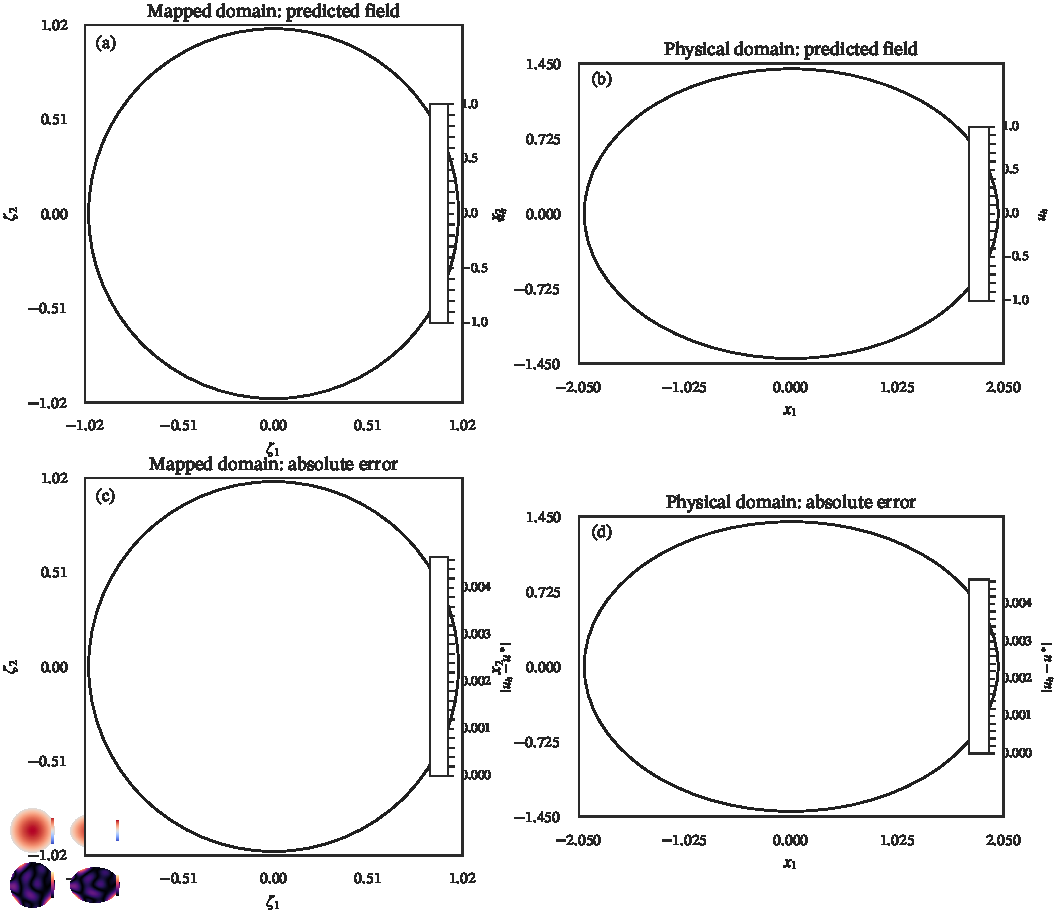
\includegraphics[width=0.97\textwidth]{figures_cmame_core/example1_forward_poisson/example1_ellipsoid_pub.png}
\caption{Ellipsoidal verification benchmark. The top row shows the predicted solution on the mapped unit-ball slice and on the corresponding physical ellipsoidal slice; the bottom row shows the absolute error in the same two coordinates. The close agreement between mapped and physical views confirms that the operator pullback and the geometric map are both implemented correctly in this analytic case.}
\label{fig:forward_poisson_ellipsoid}
\end{figure}

% Example 2 source traceability (comment only; not visible in the compiled PDF).
% Paths below are relative to the PINN_coordinate_chart_3Dgeometry/ project root.
% Code:
%   - experiments/run_poisson_rabbit_atlas_schwarz.py
%     Main chart-local PINN Schwarz solver for the fixed-atlas rabbit Poisson benchmark.
%   - experiments/run_poisson_rabbit_atlas_schwarz_fem.py
%     Atlas-based chart-local FEM variant used for the solver-portability comparison.
%   - experiments/chart_fem_solver.py
%     Local P1 tetrahedral FEM assembly/solve utilities used by the atlas-FEM rabbit study.
% Data / run artifacts:
%   - runs/atlas_vol_trained/
%     Frozen validated rabbit atlas assets (atlas data NPZ, trained decoder/mask checkpoint, gate report).
%   - runs/attempt19_w4/
%     Dense-MLP rabbit PINN benchmark run used for the reinforcement and portability comparisons.
%   - runs/attempt20c_compact/
%     CompactChartNet rabbit PINN benchmark run used for the flagship neural results and ParaView exports.
%   - runs/fem_sweep/
%     Archived atlas-FEM refinement study, including metrics, histories, and exported VTU files.
%   - runs/fem_highres/
%     High-resolution continuation of the atlas-FEM rabbit study (n=48 and n=56).
% Notes:
%   - The PDE forcing and boundary data are manufactured analytically inside the solver code.
%   - The fixed atlas assets are the geometry input for this example; the FEM baseline compares a classical chart-local discretization against the PINN on the same rabbit geometry and atlas workflow family.
\subsection{Example 2: rabbit Poisson on a fixed atlas}
\label{sec:example2}
The rabbit Poisson benchmark asks whether a fixed volumetric atlas can support a complex-geometry forward solve without being tied to a single local solver family. In the archived repository, the same atlas-based workflow supports two realizations of the mapped Poisson problem: chart-local PINN surrogates and chart-local P1 FEM solves. The physical PDE is again \eqref{eq:ex1_phys}, with
\begin{equation}
u^{\ast}_{\mathrm{rabbit}}(x)=\sin(\pi x_1)\sin(\pi x_2)\sin(\pi x_3),
\qquad
f=3\pi^2 u^{\ast}_{\mathrm{rabbit}},
\qquad
g=0.
\label{eq:rabbit_poisson_exact}
\end{equation}
The interior and boundary residuals are the same as in Example~1, but the loss adds overlap coupling:
\begin{align}
\mathcal{L}^{(2)}
=&
\lambda_{\mathrm{pde}}\sum_{i=1}^{M}\mathbb{E}_{\widehat{\Omega}_i}
\left[\left|\widehat{\mathcal{R}}^{(1)}_i\right|^2\right]
+
\lambda_{\mathrm{bc}}\sum_{i=1}^{M}\mathbb{E}_{\widehat{\Gamma}_{i,D}}
\left[\left|\widehat{\mathcal{B}}^{(1)}_{i,D}\right|^2\right]
\nonumber\\
&+
\lambda_{\mathrm{if,val}}\sum_{i<j}\mathbb{E}_{\widehat{\Omega}_{ij}}
\left[
\left|
\widehat{u}_i(\boldsymbol{\zeta})-\widehat{u}_j(\psi_{ij}(\boldsymbol{\zeta}))
\right|^2
\right]
\nonumber\\
&+
\lambda_{\mathrm{if,flux}}\sum_{i<j}\mathbb{E}_{\widehat{\Omega}_{ij}}
\left[
\left|
n_{ij}\cdot \nabla_x u_i - n_{ij}\cdot \nabla_x u_j
\right|^2
\right]
+
\lambda_{\mathrm{sup}}\mathcal{L}_{\mathrm{sup}}.
\label{eq:rabbit_poisson_loss}
\end{align}
Here $\mathcal{L}_{\mathrm{sup}}$ denotes an optional manufactured-solution anchor used in the canonical validated rabbit PINN runs to stabilize Schwarz iteration. In the current code, each chart-local neural field can be represented by a dense MLP, a residual MLP, or a compact chart-partitioned network. The validated flagship neural run uses the compact chart-partitioned architecture and is the clearest example in the release where chart-local field solves, geometry, and overlap transmission are all active simultaneously.

Example~2 is the strongest numerical evidence in the manuscript because it is the point at which geometry handling, chart-local approximation, and Schwarz transmission are all active simultaneously. The rabbit does not admit a useful low-distortion single global map in the current workflow, so the released solver instead works on a fixed 12-chart volumetric atlas constructed from SDF-interior sampling, farthest-point seed placement, overlap targeting, and geometric quality checks. Once the atlas is frozen, the PINN solver generates interior collocation by SDF rejection in chart coordinates, trains one scalar field network per chart, and enforces compatibility by interface-value and interface-flux penalties inside multiplicative Schwarz sweeps with a trust-region acceptance filter.

The repository now also contains an atlas-based FEM realization of the same benchmark. In that variant, each chart solves the same mapped Poisson operator in weak form,
\[
\int_{\widehat{\Omega}_i} (\nabla_{\boldsymbol{\zeta}} v)^T
\mathbf{A}_i(\boldsymbol{\zeta})\,
\nabla_{\boldsymbol{\zeta}} \widehat{u}_i
\,d\boldsymbol{\zeta}
=
\int_{\widehat{\Omega}_i}
j_i(\boldsymbol{\zeta})\,f(\varphi_i(\boldsymbol{\zeta}))\,v
\,d\boldsymbol{\zeta},
\]
with Dirichlet data supplied by the physical boundary and by Schwarz traces on artificial chart boundaries. Each chart uses a P1 tetrahedral discretization of the structured cube $[-r_i,r_i]^3$ split by Freudenthal tetrahedra. The implementation reuses the same decoder--mask atlas machinery, overlap coloring, and partition-of-unity blending as the PINN solver; Schwarz boundary values are again obtained from neighboring chart solutions through the atlas, and the archived FEM runs disable SDF filtering by default for these volumetric chart meshes.

The canonical compact PINN run \texttt{attempt20c\_compact} attains relative $L^2$ error $2.21\times 10^{-2}$, absolute $L^2$ error $8.57\times 10^{-3}$, maximum pointwise error $6.78\times 10^{-2}$, final interface-flux mismatch $1.16\times 10^{-2}$, and runtime $3659.0$\,s. Its archived history records $61$ Schwarz iterations, and the selected checkpoint stores twelve compact chart networks with roughly $1.31\times 10^{5}$ trainable chart-local weights in total. The diagnostics in Figures~\ref{fig:rabbit_poisson_example} and \ref{fig:rabbit_poisson_training_losses} show the same behavior spatially and temporally: the field remains smooth on the rabbit surface and the objective components contract over Schwarz iterations. A shorter dense-MLP run, \texttt{attempt19\_w4}, reaches best-checkpoint relative $L^2$ error $2.53\times 10^{-2}$ and maximum pointwise error $5.30\times 10^{-2}$ in $403.9$\,s, with a tighter archived final interface-flux mismatch of $2.52\times 10^{-3}$. The compact architecture therefore improves the best global relative $L^2$ metric and convergence smoothness, but not as a clean dominance result.

The stored run archive also contains a validated reinforcement progression that clarifies why the rabbit result is credible. The dense solver was strengthened in stages: W1 aligns evaluation with the direct-coordinate PDE operator used in training; W2 adds a manufactured-solution anchor during Schwarz sweeps; W3 drives plateau detection by evaluation relative $L^2$; W5 strengthens overlap transmission through a larger interface-flux weight and an interior overlap penalty; and W4 then applies PCGrad when the PDE and supervision gradients conflict. Table~\ref{tab:rabbit_reinforcement_progression} shows that the rabbit benchmark is therefore not a one-run anecdote. Best-checkpoint relative $L^2$ improves from $3.698\%$ at W1 to $3.165\%$ with W2 and $3.117\%$ with W3; W5 improves overlap uniformity and worst local errors more than headline global $L^2$; and W4 reduces the best dense-MLP checkpoint further to $2.531\%$. CompactChartNet reaches the best archived relative $L^2$, $2.207\%$, but at roughly nine times the runtime of \texttt{attempt19\_w4} and with a larger maximum pointwise error.

\begin{table}[htbp]
\centering
\scriptsize
\setlength{\tabcolsep}{3pt}
\caption{Archived reinforcement progression for the rabbit Poisson benchmark. The dense-MLP study is cumulative: W1 aligns evaluation with the direct-coordinate PDE operator used in training, W2 adds manufactured-solution anchoring during Schwarz, W3 drives plateau detection by the evaluation relative $L^2$, W5 strengthens overlap coupling, and W4 applies PCGrad to the PDE-versus-anchor conflict. Relative $L^2$ and maximum pointwise error are reported for the selected best-rel-$L^2$ checkpoint of each run; runtime is the total archived run time.}
\label{tab:rabbit_reinforcement_progression}
\begin{tabular}{>{\raggedright\arraybackslash}p{1.7cm}>{\raggedright\arraybackslash}p{4.15cm}>{\centering\arraybackslash}p{1.28cm}>{\centering\arraybackslash}p{1.28cm}>{\centering\arraybackslash}p{1.15cm}}
\toprule
Run & Added ingredient & Best rel.\ $L^2$ & Max error & Runtime \\
\midrule
\texttt{attempt15b\_w1} & W1: direct-coordinate PDE evaluation and consistent scoring & 3.698\% & 4.107\% & 364\,s \\
\texttt{attempt16\_w2} & + W2: manufactured-solution anchor during Schwarz & 3.165\% & 4.993\% & 335\,s \\
\texttt{attempt17\_w3} & + W3: plateau detection driven by rel.\ $L^2$ & 3.117\% & 8.485\% & 328\,s \\
\texttt{attempt18\_w5} & + W5: stronger flux coupling and overlap penalty & 3.631\% & 5.450\% & 371\,s \\
\texttt{attempt19\_w4} & + W4: PCGrad on the PDE/supervision conflict & 2.531\% & 5.303\% & 404\,s \\
\shortstack[l]{\texttt{attempt20c}\\ \texttt{\_compact}} & CompactChartNet with all W1--W5 features active & \textbf{2.207\%} & 6.783\% & 3659\,s \\
\bottomrule
\end{tabular}
\end{table}

The new FEM baseline makes the rabbit solver comparison concrete rather than hypothetical. Table~\ref{tab:rabbit_fem_convergence} reports the full archived $h$-refinement study from $n_{\mathrm{cells}}=8$ to $56$. The relative $L^2$ error drops from $5.47\times 10^{-1}$ to $1.79\times 10^{-2}$, and the observed rates approach the theoretical $O(h^2)$ behavior of mapped P1 elements on the frozen atlas. Figure~\ref{fig:rabbit_poisson_fem_refinement} shows the same trend visually: the FEM curve intersects the compact PINN reference near $n_{\mathrm{cells}}=48$ and moves below it at $n_{\mathrm{cells}}=56$.

\begin{table}[htbp]
\centering
\scriptsize
\setlength{\tabcolsep}{3.0pt}
\caption{Atlas-based FEM $h$-refinement study for the rabbit Poisson benchmark. Rates are computed between successive archived levels using the relative-$L^2$ error.}
\label{tab:rabbit_fem_convergence}
\begin{tabular}{>{\centering\arraybackslash}p{0.72cm}>{\centering\arraybackslash}p{1.0cm}>{\centering\arraybackslash}p{1.48cm}>{\centering\arraybackslash}p{1.28cm}>{\centering\arraybackslash}p{0.82cm}>{\centering\arraybackslash}p{1.18cm}>{\centering\arraybackslash}p{0.74cm}}
\toprule
$n_{\mathrm{cells}}$ & $h$ & DOFs & rel.\ $L^2$ & Rate & Max error & Time \\
\midrule
8  & $9.31\times10^{-2}$ & 5{,}832     & $5.47\times10^{-1}$ & ---  & $2.42\times10^{-1}$ & 7\,s \\
16 & $4.65\times10^{-2}$ & 39{,}304    & $2.00\times10^{-1}$ & 1.45 & $9.04\times10^{-2}$ & 45\,s \\
24 & $3.10\times10^{-2}$ & 125{,}000   & $9.49\times10^{-2}$ & 1.84 & $4.47\times10^{-2}$ & 5\,min \\
32 & $2.33\times10^{-2}$ & 287{,}496   & $5.55\times10^{-2}$ & 1.86 & $2.64\times10^{-2}$ & 21\,min \\
48 & $1.55\times10^{-2}$ & 941{,}192   & $2.48\times10^{-2}$ & 1.99 & $1.12\times10^{-2}$ & 49\,min \\
56 & $1.33\times10^{-2}$ & 1{,}481{,}544 & $\mathbf{1.79\times10^{-2}}$ & 2.10 & $\mathbf{8.72\times10^{-3}}$ & 140\,min \\
\bottomrule
\end{tabular}
\end{table}

\begin{table}[htbp]
\centering
\scriptsize
\setlength{\tabcolsep}{3.0pt}
\caption{Head-to-head rabbit comparison on the frozen atlas workflow. The compact PINN row reports the selected best-rel-$L^2$ checkpoint; the FEM rows report archived final metrics after five Schwarz sweeps. The FEM artifacts are stored as 8-chart runs, while the compact PINN uses the validated 12-chart rabbit atlas.}
\label{tab:rabbit_solver_comparison}
\begin{tabular}{>{\raggedright\arraybackslash}p{1.45cm}>{\centering\arraybackslash}p{0.75cm}>{\raggedright\arraybackslash}p{1.95cm}>{\centering\arraybackslash}p{1.12cm}>{\centering\arraybackslash}p{1.12cm}>{\centering\arraybackslash}p{0.72cm}>{\centering\arraybackslash}p{0.88cm}}
\toprule
Local solver & Charts & Size & rel.\ $L^2$ & Max error & Sweeps & Runtime \\
\midrule
PINN compact & 12 & $1.31\times10^{5}$ weights & $2.21\times10^{-2}$ & $6.78\times10^{-2}$ & 61 & 3659\,s \\
\shortstack[l]{FEM P1\\($n=48$)} & 8 & $9.41\times10^{5}$ DOFs & $2.48\times10^{-2}$ & $1.12\times10^{-2}$ & 5 & 2939\,s \\
\shortstack[l]{FEM P1\\($n=56$)} & 8 & $1.48\times10^{6}$ DOFs & $\mathbf{1.79\times10^{-2}}$ & $\mathbf{8.72\times10^{-3}}$ & 5 & 8395\,s \\
\bottomrule
\end{tabular}
\end{table}

Table~\ref{tab:rabbit_solver_comparison} clarifies the tradeoff along several axes. At $n_{\mathrm{cells}}=48$, the atlas-FEM error $2.48\times 10^{-2}$ is already comparable to the compact PINN's $2.21\times 10^{-2}$, and at $n_{\mathrm{cells}}=56$ it improves that metric by about $19\%$. In wall-clock time the two methods are broadly competitive at matched accuracy: the FEM reaches $2.48\times 10^{-2}$ in $2{,}939$\,s versus the PINN's $2.21\times 10^{-2}$ in $3{,}659$\,s. Surpassing the PINN with the FEM requires the $n=56$ level at $8{,}395$\,s, indicating that the atlas-plus-Schwarz infrastructure is the dominant cost driver in both cases, not the local PDE discretization itself.

The Schwarz behavior is qualitatively different. The FEM branch converges in five sweeps because each chart solves a sparse linear system by direct factorization, while inter-chart Schwarz boundary data require Newton inversion of the nonlinear decoder map $\varphi_j^{-1}$. These inversions are precomputed once per resolution level and cached, since they depend only on the atlas geometry and not on the evolving solution. The PINN branch instead evaluates its field directly in the rigid local coordinates, avoiding decoder inversion entirely, but at the expense of a longer gradient-based Schwarz history ($61$ sweeps) and ${\sim}200$ local optimizer steps per chart per sweep.

A revealing comparison metric is the total number of neural-network forward passes through the shared decoder and mask networks. The FEM solver queries these networks only during the one-time geometric precomputation---Newton-based map inversions at artificial boundary nodes and mask-logit evaluations for partition-of-unity weights---amounting to approximately $23$ million forward passes at $n=48$, performed once and cached. The SA-PINN evaluates its chart-local field networks and their autograd derivatives at every training step across all Schwarz sweeps: with $61$ sweeps, ${\sim}200$ local steps per chart, $8$ active charts, and ${\sim}2{,}000$ collocation points per step, the total reaches approximately $195$ million neural-network evaluations, roughly $8.5\times$ the FEM count. This disparity quantifies the fundamental cost difference: the PINN pays for approximation power through iterative training, while the FEM amortizes geometry queries into a one-time precomputation and pays instead through mesh refinement.

Most importantly, the FEM convergence study in Table~\ref{tab:rabbit_fem_convergence} serves as an independent validation of the atlas-based coordinate pullback. The observed $O(h^2)$ rates---approaching the theoretical expectation for P1 elements---confirm that the mapped diffusion tensor $\mathbf{A}_i = j_i \mathbf{J}_i^{-1}\mathbf{J}_i^{-T}$, the Jacobian-weighted load vector, and the Schwarz boundary exchange introduce no spurious accuracy degradation. This is a statement about the geometric infrastructure, not about either solver: the atlas is mathematically faithful as a coordinate substrate. The rabbit benchmark therefore supports a sharper conclusion than before: the atlas is discretization-agnostic, and the FEM convergence independently certifies the correctness of the mapped-operator formulation.

\begin{figure}[htbp]
\centering
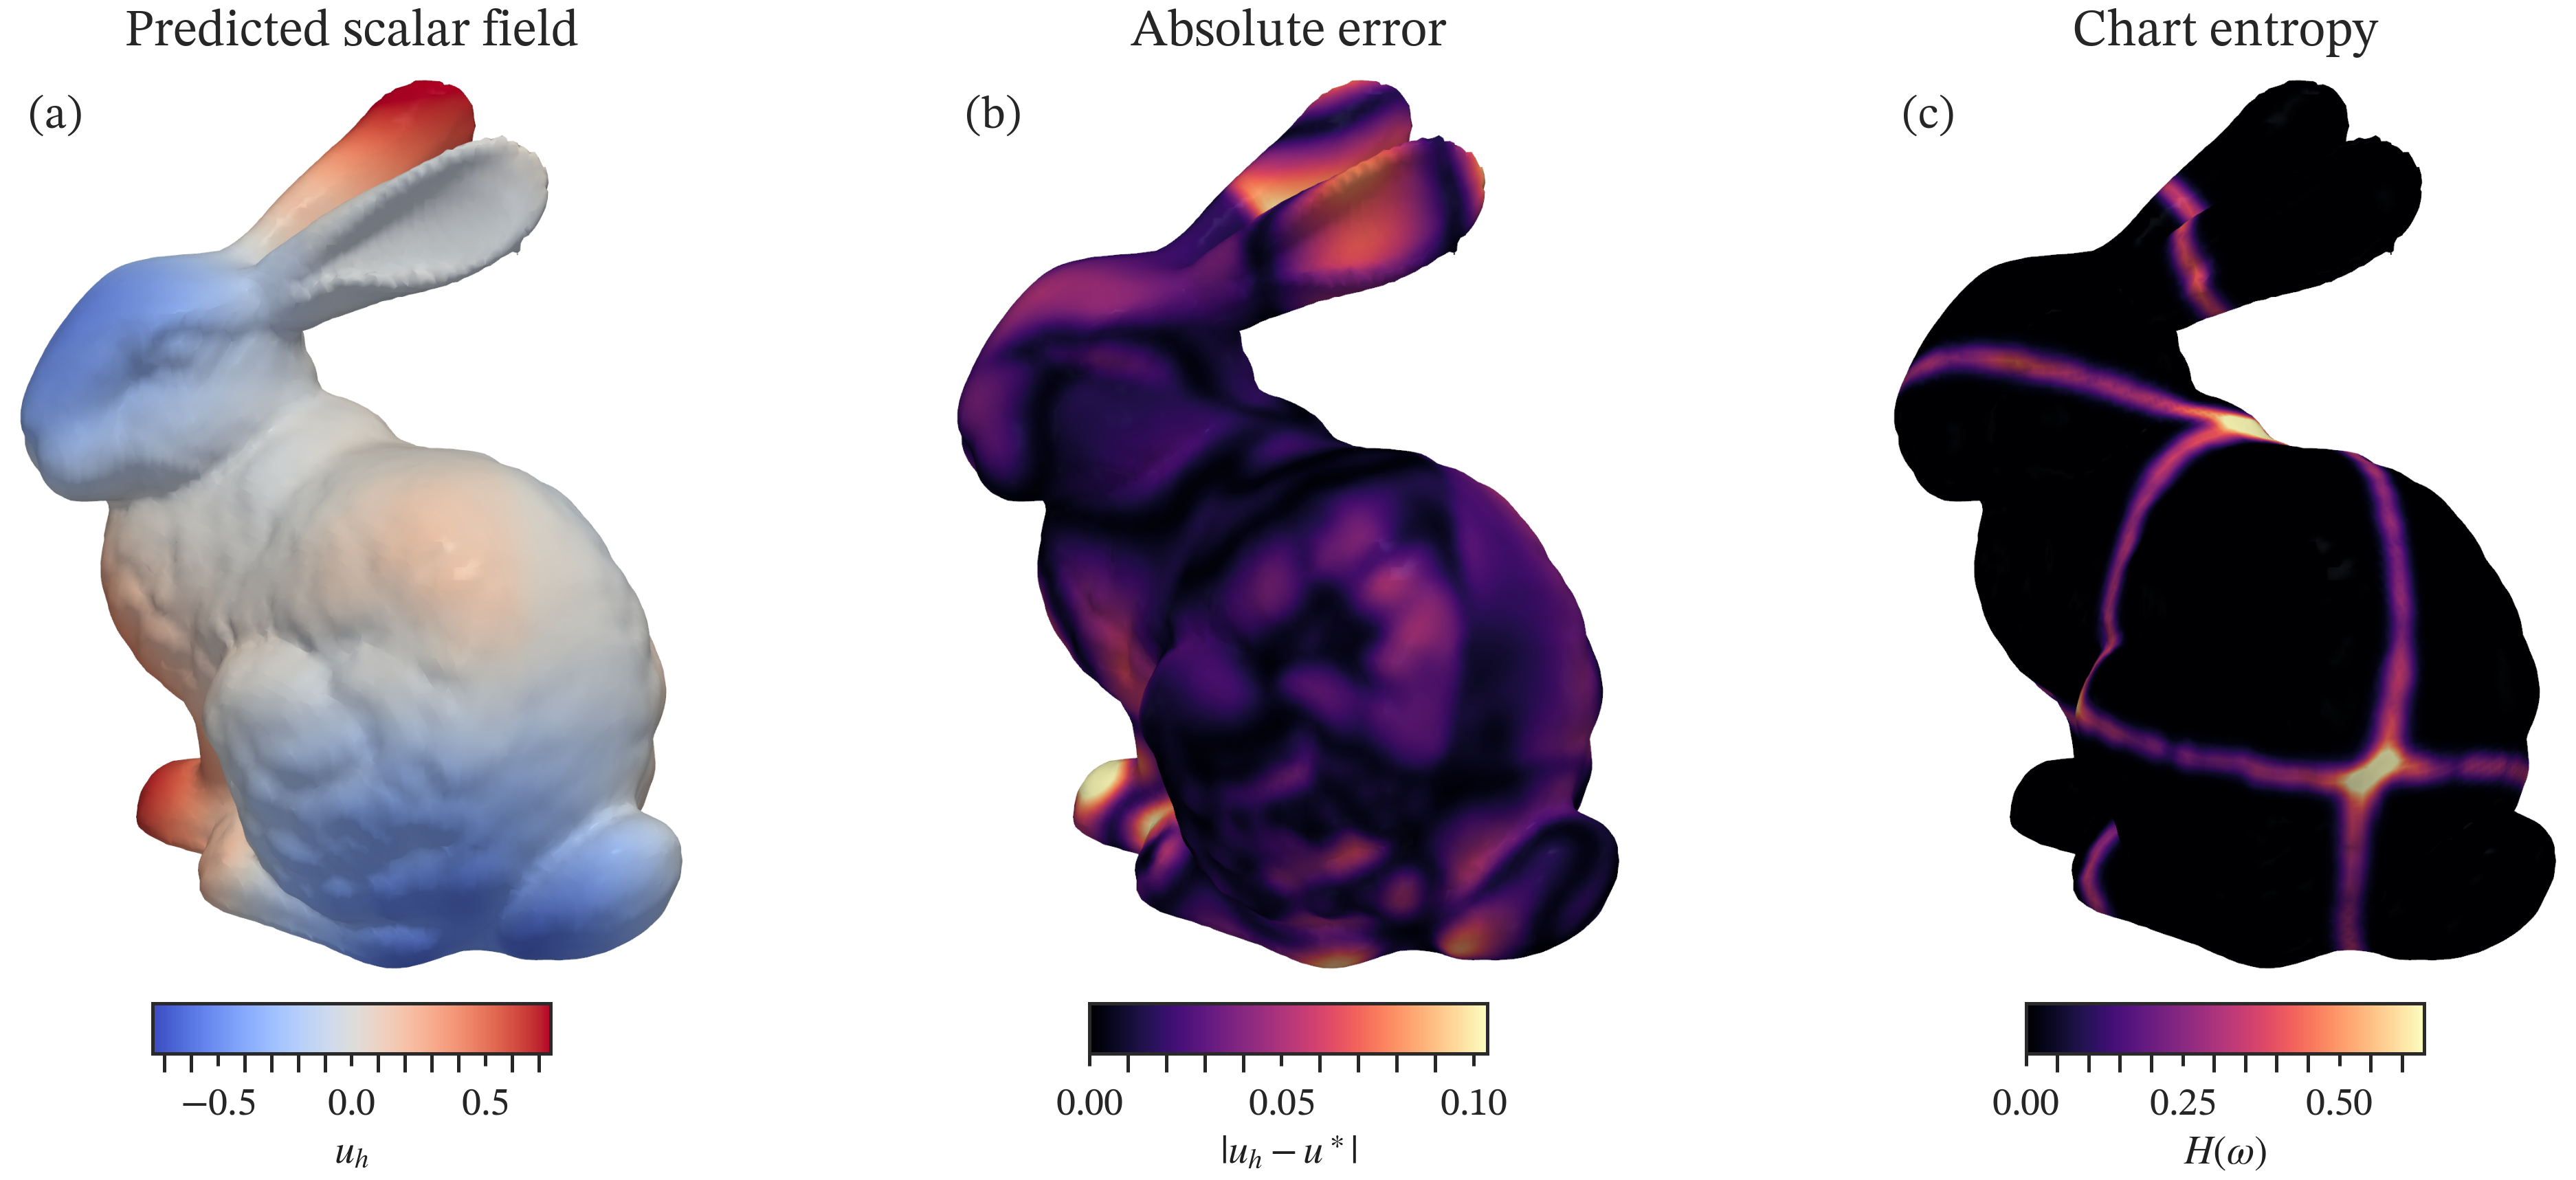
\includegraphics[width=0.98\textwidth]{figures_cmame_core/example2_rabbit_poisson/example2_rabbit_poisson_pub.png}
\caption{Representative rabbit-surface visualization for the fixed-atlas SA-PINN solver. The surface is reconstructed from a dense boundary postprocessing pass of the rabbit Poisson solution family and shown from one fixed camera in all three panels. Panel (a) shows the recovered scalar field, panel (b) shows the absolute error, and panel (c) shows the chart entropy induced by the partition-of-unity weights. The first two panels show that the solved field remains smooth on the complex geometry, while the entropy panel shows that uncertainty is confined to narrow overlap traces rather than spreading over the whole surface.}
\label{fig:rabbit_poisson_example}
\end{figure}

The canonical archive stores the global Schwarz objective components at every iteration, but it does not preserve chart-resolved loss histories over time. For that reason, the diagnostics below separate the archived scalar PINN losses from the independently archived FEM refinement sweep. This avoids conflating the raw loss scales used for neural checkpointing with the mesh-refinement evidence used to assess solver-level comparison on the rabbit geometry.

\begin{figure}[htbp]
\centering
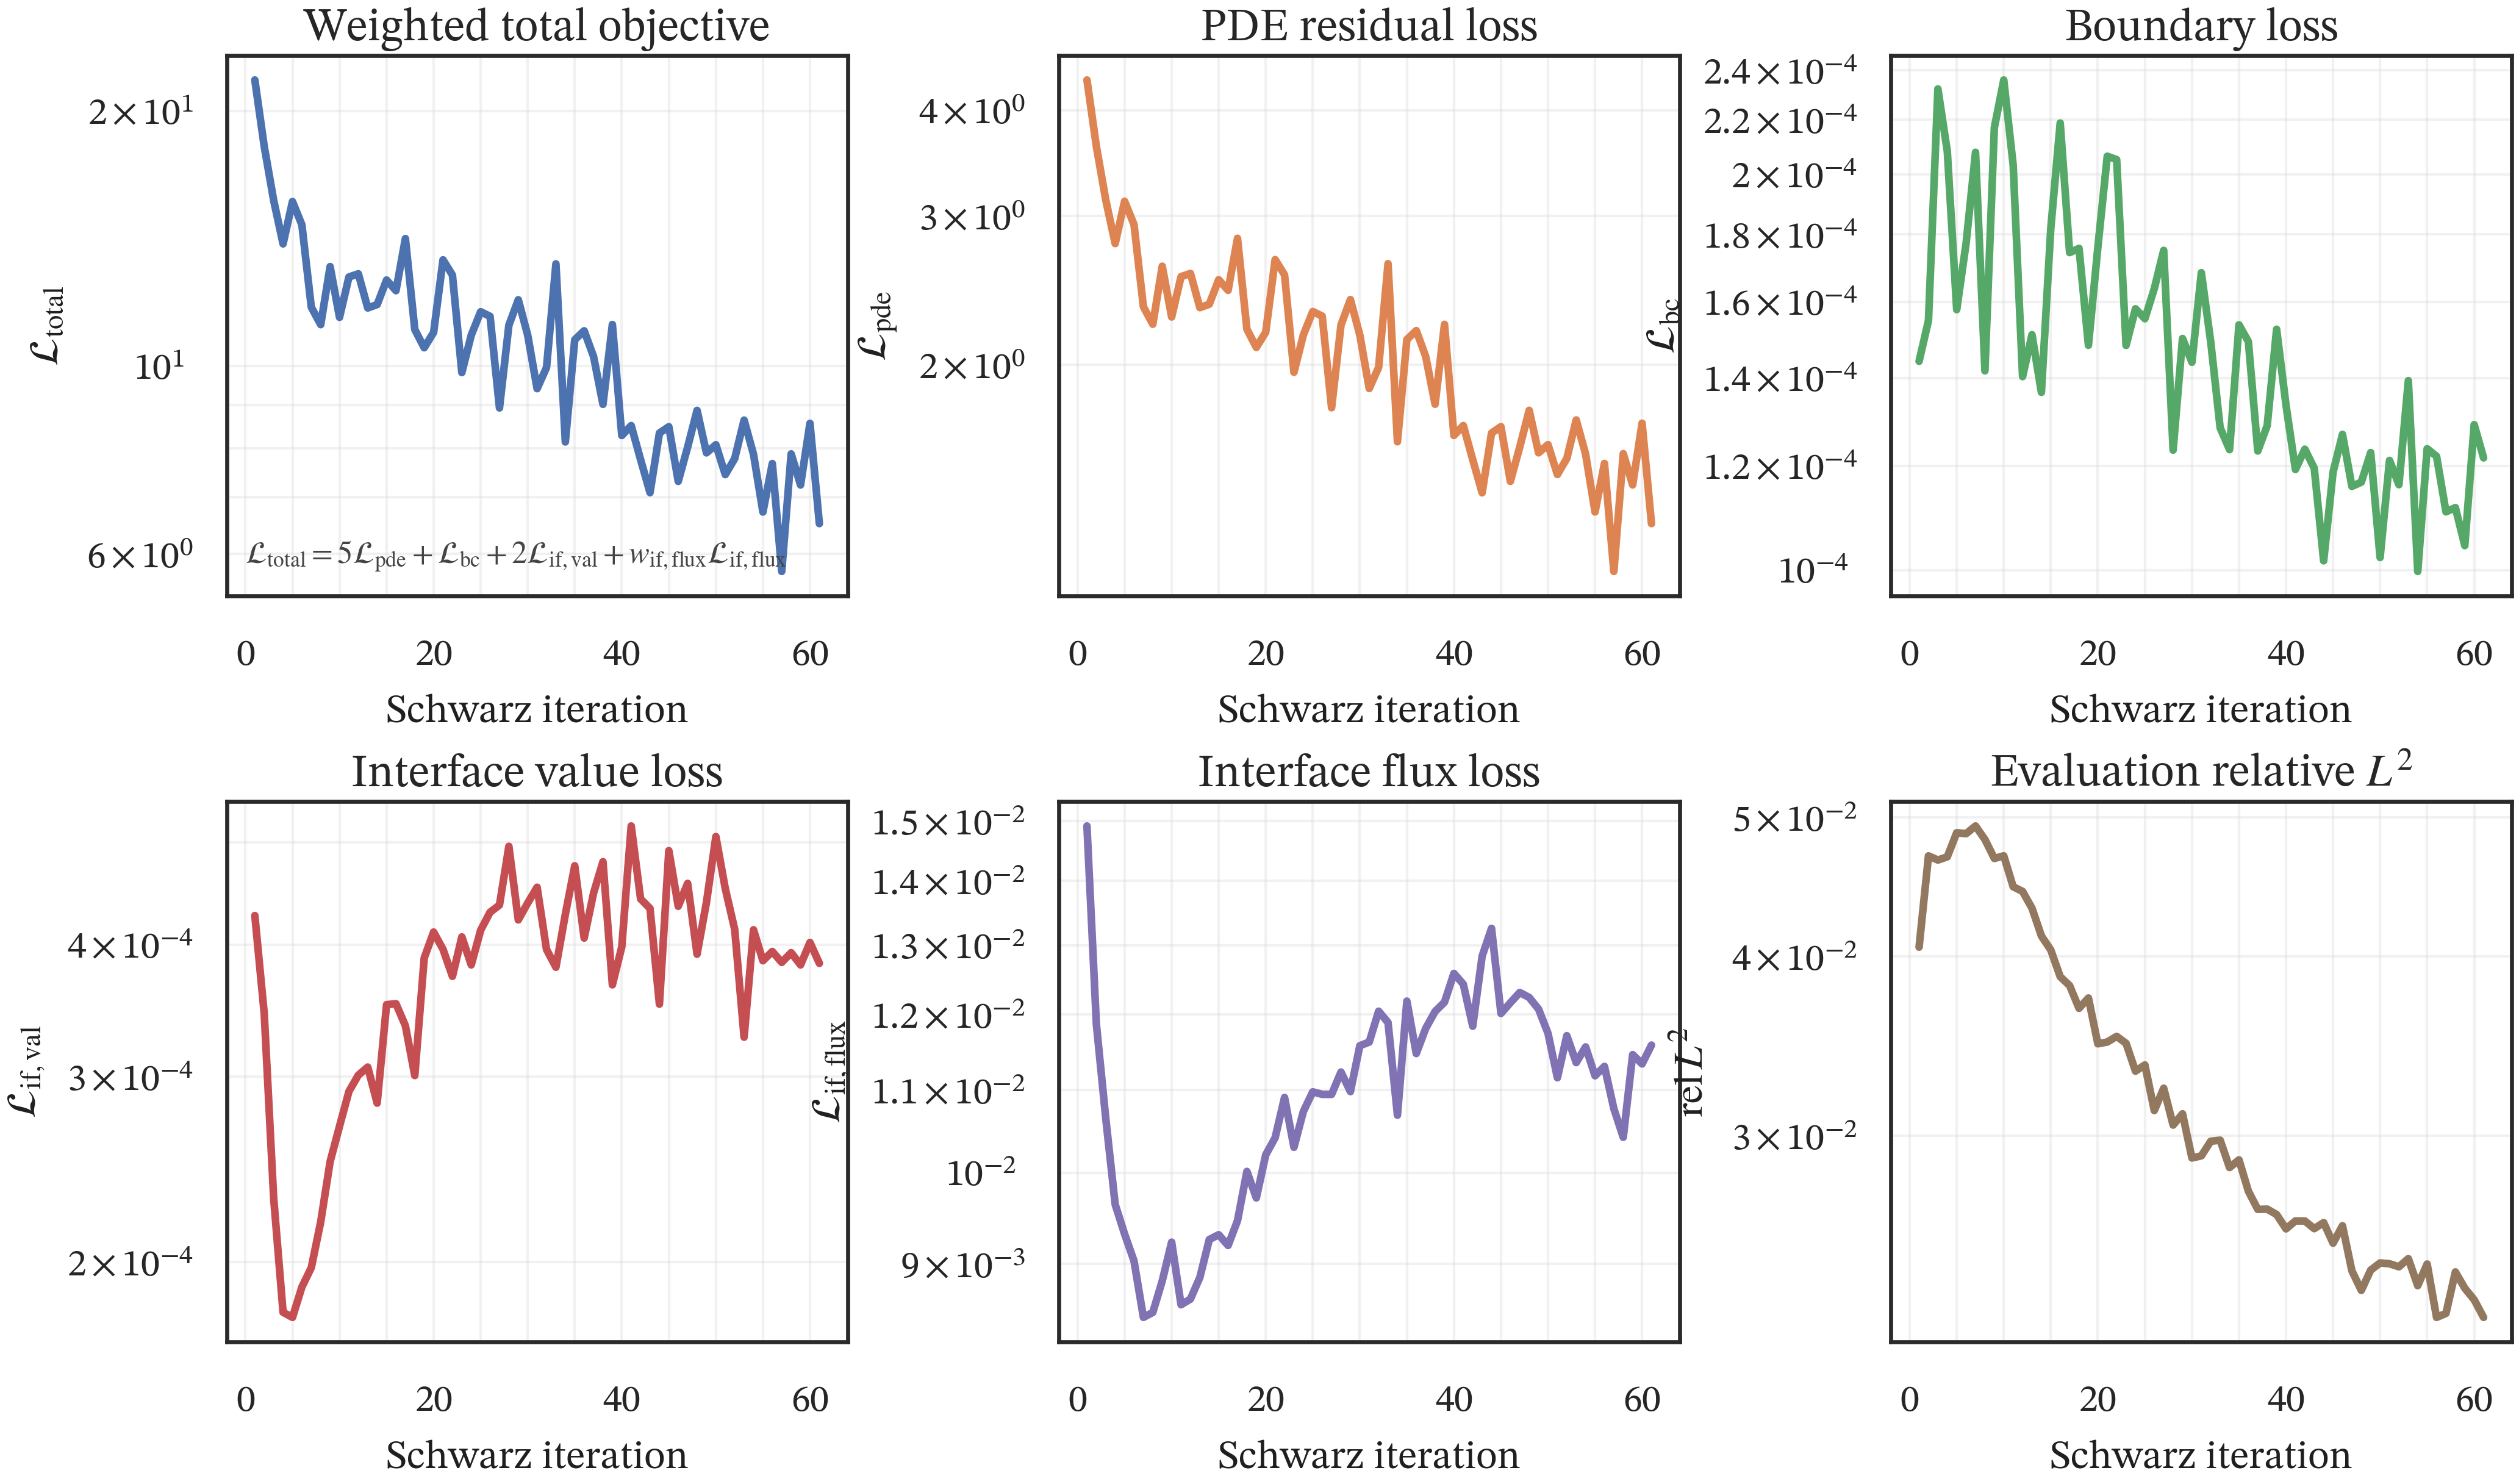
\includegraphics[width=0.98\textwidth]{figures_cmame_core/example2_rabbit_poisson/example2_rabbit_poisson_losses_pub.png}
\caption{Archived training diagnostics for the canonical rabbit Poisson run \texttt{attempt20c\_compact}. Each panel reports one scalar trace recorded over Schwarz iterations: the weighted total objective used by the solver, the PDE residual loss, the boundary loss, the interface-value loss, the interface-flux loss, and the evaluation relative $L^2$ error. Presenting these quantities in separate panels makes the balance between objectives easier to read than an overlaid weighted-objective plot, while still documenting the aggregate score used in the implementation.}
\label{fig:rabbit_poisson_training_losses}
\end{figure}

\begin{figure}[htbp]
\centering
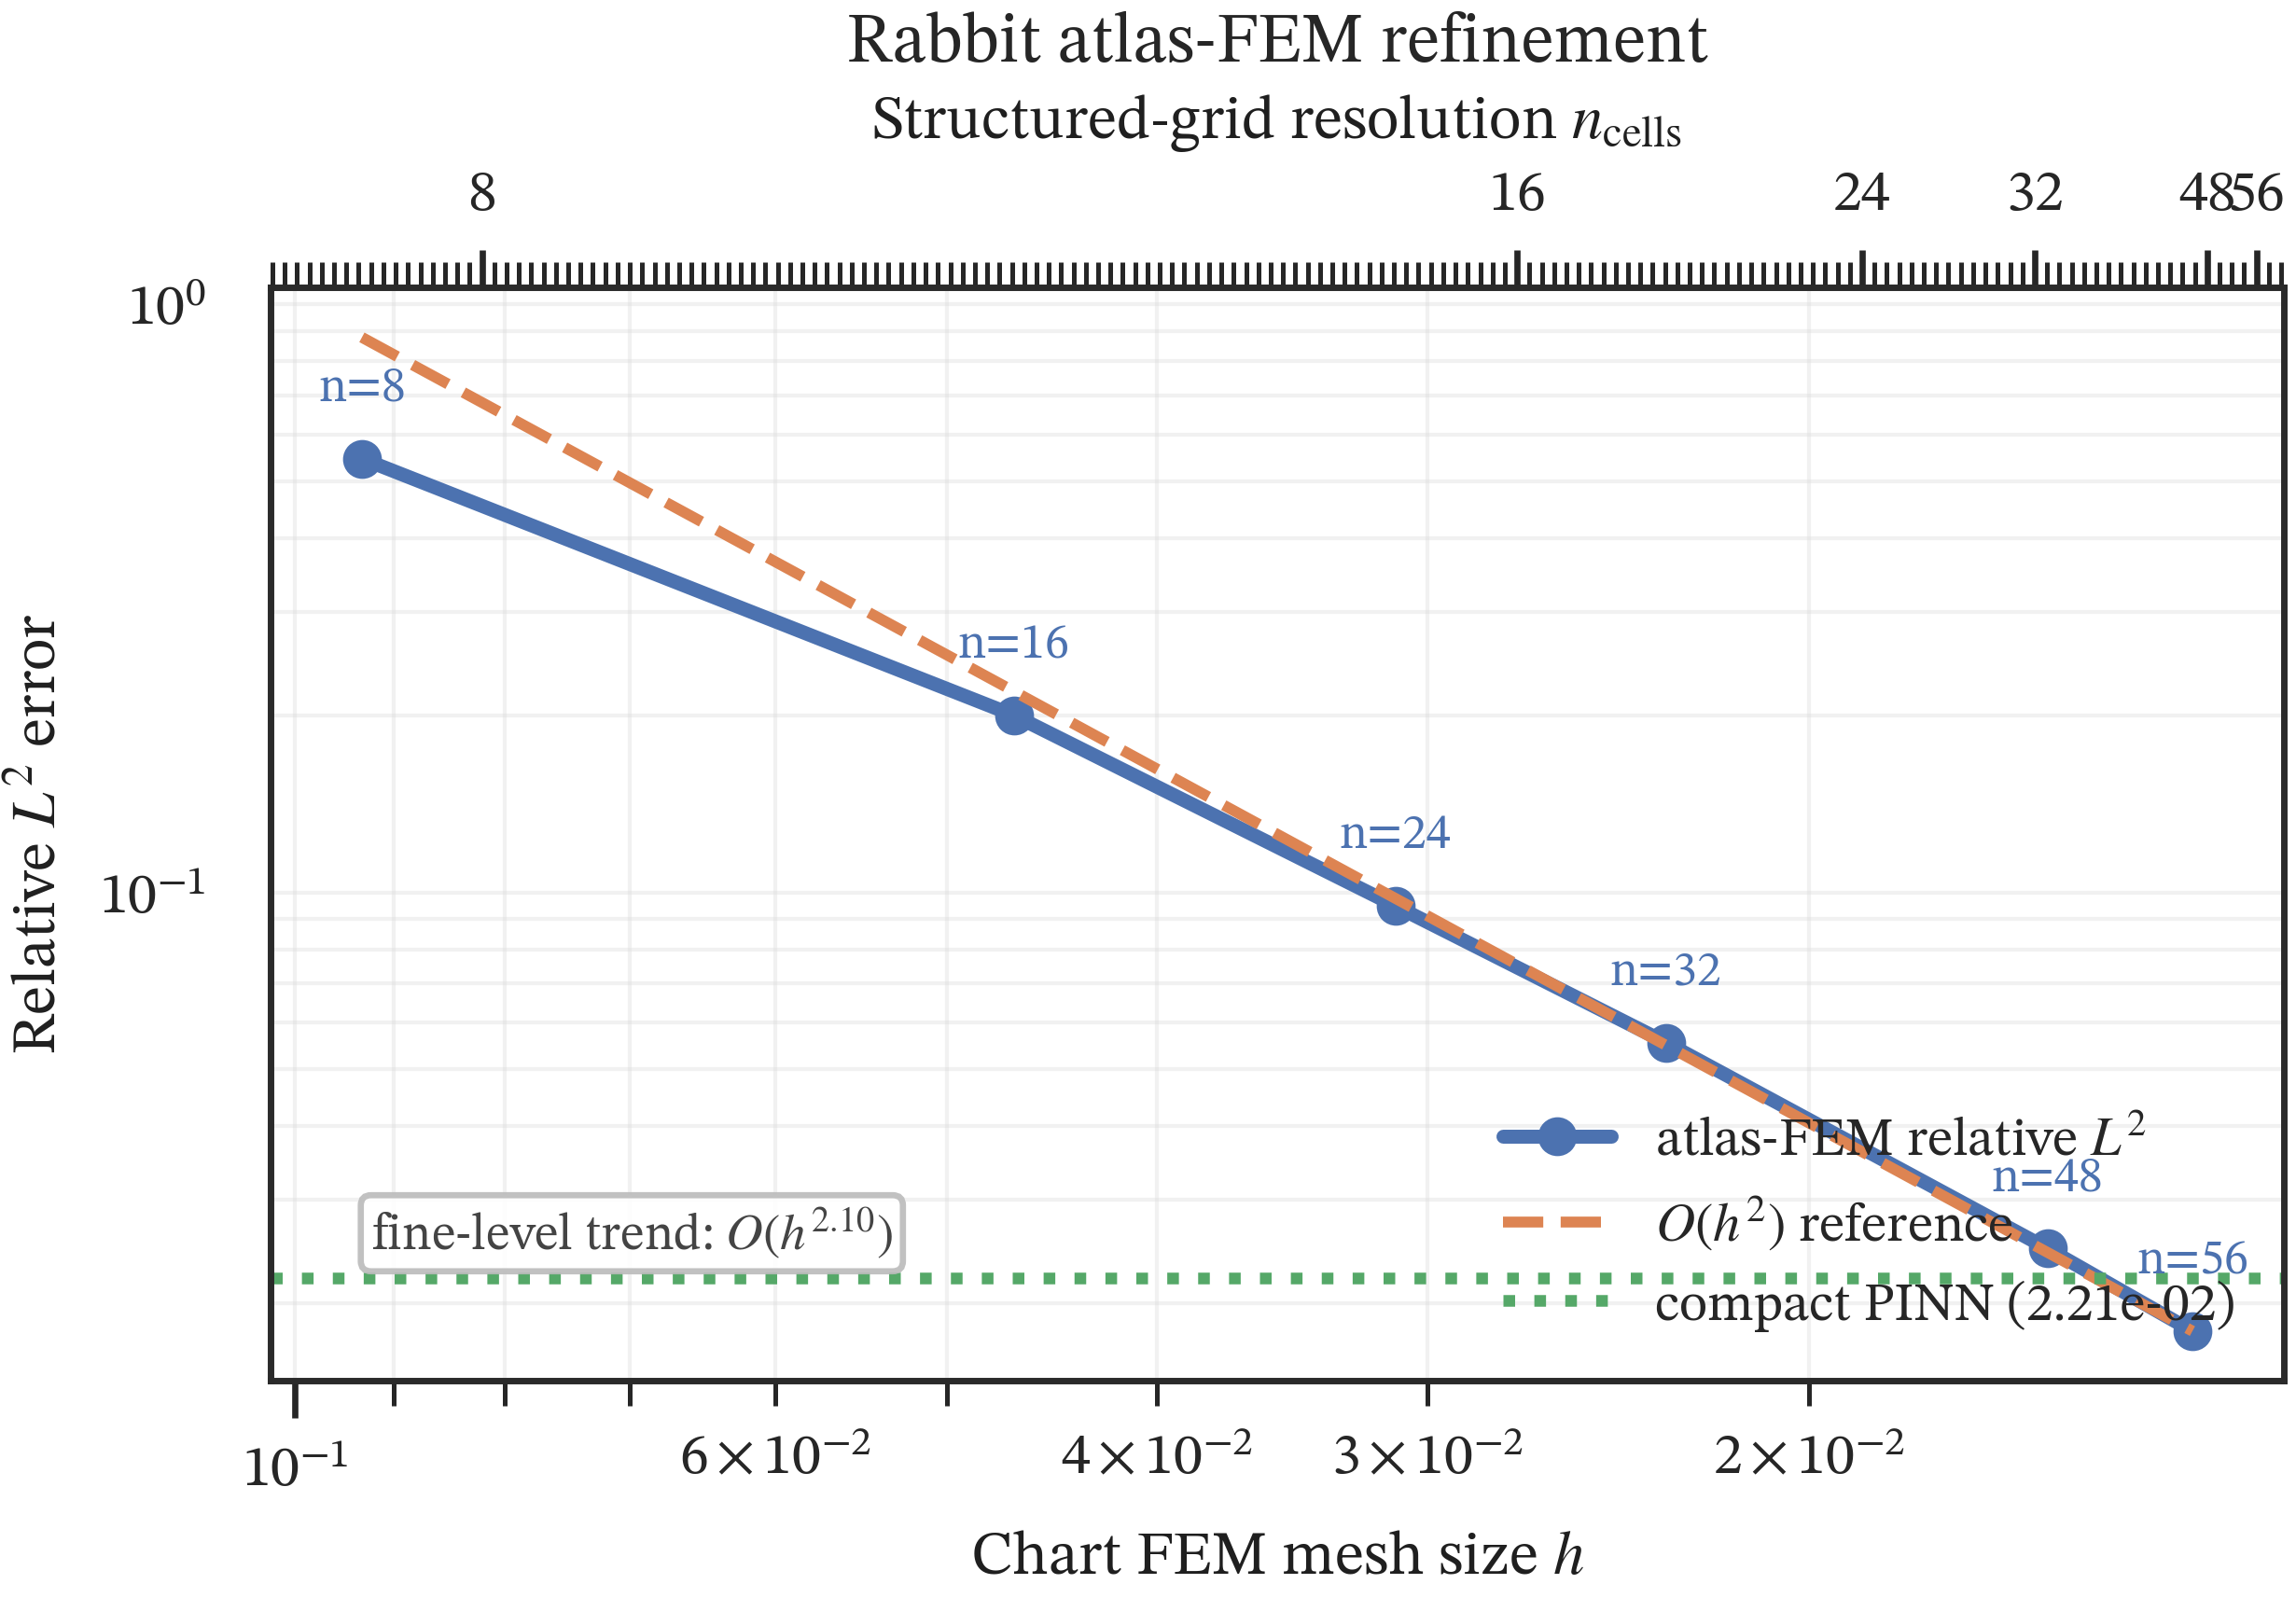
\includegraphics[width=0.68\textwidth]{figures_cmame_core/example2_rabbit_poisson/example2_rabbit_poisson_fem_refinement_pub.png}
\caption{Atlas-based FEM convergence on the rabbit benchmark. The plotted curve uses the archived $h$-refinement sequence $n_{\mathrm{cells}}=8,16,24,32,48,56$ and shows the relative-$L^2$ error of the chart-local P1 FEM solve on the frozen rabbit atlas workflow. The dashed line gives an $O(h^2)$ reference slope, and the dotted horizontal line marks the compact PINN accuracy $2.21\times10^{-2}$. The FEM trajectory matches that level near $n_{\mathrm{cells}}=48$ and improves beyond it at $n_{\mathrm{cells}}=56$, which is consistent with the expected asymptotic behavior of mapped P1 elements.}
\label{fig:rabbit_poisson_fem_refinement}
\end{figure}

For traceability, the lower sweep levels in Figure~\ref{fig:rabbit_poisson_fem_refinement} are also available as archived ParaView exports. Table~\ref{tab:rabbit_fem_refinement_artifacts} lists the exported VTU files for the original $n_{\mathrm{cells}}=8,16,24,32$ sweep together with the stored error metrics and the accompanying manifest file; the finer $n_{\mathrm{cells}}=48$ and $56$ points come from the archived high-resolution metric files in \texttt{runs/fem\_highres/}.

\begin{table}[htbp]
\centering
\scriptsize
\setlength{\tabcolsep}{3.2pt}
\caption{Archived ParaView outputs for the rabbit atlas-FEM refinement study. The VTU rows correspond to the exported field at each stored FEM resolution; the manifest records the export set.}
\label{tab:rabbit_fem_refinement_artifacts}
\begin{tabular}{>{\raggedright\arraybackslash}p{3.55cm}>{\centering\arraybackslash}p{1.0cm}>{\centering\arraybackslash}p{1.15cm}>{\centering\arraybackslash}p{1.15cm}}
\toprule
File & $n_{\mathrm{cells}}$ & rel.-$L^2$ & max-error \\
\midrule
\texttt{fem\_poisson\_n8.vtu} & 8 & $5.47\times 10^{-1}$ & $2.42\times 10^{-1}$ \\
\texttt{fem\_poisson\_n16.vtu} & 16 & $2.00\times 10^{-1}$ & $9.04\times 10^{-2}$ \\
\texttt{fem\_poisson\_n24.vtu} & 24 & $9.49\times 10^{-2}$ & $4.47\times 10^{-2}$ \\
\texttt{fem\_poisson\_n32.vtu} & 32 & $5.55\times 10^{-2}$ & $2.64\times 10^{-2}$ \\
\texttt{fem\_paraview\_manifest.json} & --- & manifest & --- \\
\bottomrule
\end{tabular}
\end{table}

% Example 3 source traceability (comment only; not visible in the compiled PDF).
% Paths below are relative to the PINN_coordinate_chart_3Dgeometry/ project root.
% Code:
%   - src/train_sdf_rabbit.py
%     Main global volumetric Bunny SDF trainer used for the canonical geometry-learning benchmark.
%   - experiments/run_poisson_rabbit_atlas_schwarz.py
%     Reused for the downstream 8-chart Bunny Poisson continuation study discussed in this example.
% Data / run artifacts:
%   - runs/atlas_schwarz_20260212_210412/downloads/bunny/reconstruction/bun_zipper.ply
%     Imported watertight Stanford Bunny surface mesh used as the raw geometry input.
%   - runs/bunny_sdf_v3/
%     Canonical archived global Bunny volumetric SDF run (checkpoint, history, slice plot, metadata).
%   - runs/atlas_bunny_repaired_8chart/
%     Repaired 8-chart Bunny atlas used for the downstream continuation study.
%   - runs/bunny_poisson_8chart*
%     Family of downstream Bunny Poisson continuation runs that vary interior supervised pretraining.
%   - paraview/bunny_poisson_8chart_intpre20k/
%     Best archived continuation export package used for the Example 3 surface visualization.
% Notes:
%   - This example combines geometry learning and supporting continuation evidence: the first part is the
%     global SDF benchmark, while the second part checks whether the learned/repaired Bunny geometry can feed a downstream solve.
\subsection{Example 3: Stanford Bunny PLY volumetric neural SDF benchmark}
\label{sec:example3}
The Stanford Bunny benchmark is the geometry-learning example of the paper. Its input is an oriented surface sample set
\[
X_{\partial}=\{(x_k,n_k)\}_{k=1}^{N_s}
\]
obtained from the watertight Stanford Bunny mesh \texttt{bun\_zipper.ply}. The goal is not to reconstruct only a surface mesh, but to learn a volumetric scalar field whose zero level set captures the Bunny surface and whose sign defines a usable interior for later atlas construction. In that sense, this example should be read as the benchmark instantiation of Stage~1 in Section~\ref{sec:impl_pipeline}: it asks whether an imported PLY surface can be converted into a differentiable volumetric geometry model.

Let
\begin{equation}
y=\frac{x-c}{s}\in \mathbb{R}^3
\label{eq:bunny_sdf_normalized_coord}
\end{equation}
denote the normalized coordinate used in the code, where $c$ is the bounding-box center and $s$ is the global length scale extracted from the point cloud. This normalization is not cosmetic. It keeps the Bunny inside an $O(1)$ box, makes the surface and Eikonal samples live on comparable scales, and allows the same network widths and sampling ranges to be reused without geometry-dependent retuning. The learned volumetric model is a scalar network
\begin{equation}
s_\theta:\mathbb{R}^3\rightarrow \mathbb{R}
\label{eq:bunny_sdf_network}
\end{equation}
from which the reconstructed body is defined by
\begin{equation}
\Omega_\theta=\{x:s_\theta((x-c)/s)<0\},
\qquad
\partial\Omega_\theta=\{x:s_\theta((x-c)/s)=0\}.
\label{eq:bunny_sdf_body}
\end{equation}
Equations~\eqref{eq:bunny_sdf_network}--\eqref{eq:bunny_sdf_body} define the actual learned geometric object. The network output is a volumetric level-set field, not a surface patch parametrization, and the sign of that field is what later drives interior queries, chart placement, and blend evaluation. The learning objective is therefore volumetric: the zero set should approximate the observed surface, the gradient should align with the observed normals, and the field should behave approximately like a signed-distance function away from the surface.

For the normalized surface samples $\{(y_k,n_k)\}_{k=1}^{N_s}$ and randomly sampled off-surface points, the implemented loss has four parts. The surface and normal-alignment terms are
\begin{equation}
\mathcal{L}_{\mathrm{surf}}
=
\frac{1}{N_s}\sum_{k=1}^{N_s}\left|s_\theta(y_k)\right|,
\qquad
\mathcal{L}_{\mathrm{norm}}
=
\frac{1}{N_s}\sum_{k=1}^{N_s}\left(1-\widehat{\nabla_y s_\theta}(y_k)\cdot n_k\right),
\label{eq:bunny_sdf_surface_normal}
\end{equation}
where $\widehat{\nabla_y s_\theta}=\nabla_y s_\theta/\|\nabla_y s_\theta\|$. These two terms serve different purposes. The surface term pins the zero level set to the observed Bunny surface, while the normal term orients that zero set correctly and suppresses solutions that fit the points but carry the wrong local normal direction. The Eikonal term is
\begin{equation}
\mathcal{L}_{\mathrm{eik}}
=
\frac{1}{N_e}\sum_{m=1}^{N_e}
\left(\|\nabla_y s_\theta(\tilde y_m)\|_2-1\right)^2,
\label{eq:bunny_sdf_eikonal}
\end{equation}
which regularizes the field away from the surface toward signed-distance behavior. This term matters because the later atlas builder does not query only the zero set; it also queries the field and its gradient in the surrounding volume. The sign-anchor term is enforced by offsetting surface points along the known normals:
\begin{equation}
\mathcal{L}_{\mathrm{sign}}
=
\frac{1}{2N_s}\sum_{k=1}^{N_s}
\left[
\operatorname{softplus}\!\big(s_\theta(y_k-\delta n_k)\big)
\;+\;
\operatorname{softplus}\!\big(-s_\theta(y_k+\delta n_k)\big)
\right]
\;+\;
\mathcal{L}_{\mathrm{far}},
\label{eq:bunny_sdf_sign}
\end{equation}
where $\delta$ is the anchor offset and $\mathcal{L}_{\mathrm{far}}$ encourages positive SDF values well outside the body. The role of \eqref{eq:bunny_sdf_sign} is topological rather than geometric: it tries to keep the sign of the level-set field consistent just inside and just outside the observed surface. On thin features such as the Bunny ears, this is the most fragile part of the objective because one global offset $\delta$ can easily step across the local thickness of the geometry. The total loss is
\begin{equation}
\mathcal{L}^{(3)}
=
\lambda_{\mathrm{surf}}\mathcal{L}_{\mathrm{surf}}
\,+\,
\lambda_{\mathrm{eik}}\mathcal{L}_{\mathrm{eik}}
\,+\,
\lambda_{\mathrm{norm}}\mathcal{L}_{\mathrm{norm}}
\,+\,
\lambda_{\mathrm{sign}}\mathcal{L}_{\mathrm{sign}}.
\label{eq:bunny_sdf_loss}
\end{equation}
Equation~\eqref{eq:bunny_sdf_loss} is a scalarization of a genuinely multi-objective geometry problem. The near-surface terms $\mathcal{L}_{\mathrm{surf}}$ and $\mathcal{L}_{\mathrm{norm}}$ reward local surface fidelity, whereas $\mathcal{L}_{\mathrm{eik}}$ and $\mathcal{L}_{\mathrm{sign}}$ promote globally consistent volumetric behavior. These objectives can conflict, especially on thin features, and the released global Bunny trainer \texttt{train\_sdf\_rabbit.py} does not use GradNorm, PCGrad, or any other explicit conflict-mitigation scheme. Instead it relies on normalization, sampling design, and static loss weights, which is why the canonical run should be read as a baseline geometry-learning bridge rather than as a fully stabilized volumetric reconstruction method.

Example~3 therefore asks a focused question: can an imported PLY surface be converted into a differentiable volumetric geometry model that is usable for downstream atlas construction? The released Bunny script normalizes the point cloud, trains a single scalar network $s_\theta$ from surface points and normals, and balances surface fitting, normal alignment, Eikonal regularization, and sign-anchor supervision. The output is not only a surface fit; it is a volumetric level-set field whose zero contour approximates the Bunny surface and whose sign is later used to define the interior for chart placement and blend evaluation.

The canonical run \texttt{bunny\_sdf\_v3} reduces the surface loss from $6.45\times 10^{-2}$ to $1.66\times 10^{-2}$ and the normal-alignment loss from $1.01$ to $3.18\times 10^{-2}$, while the sign-anchor loss decreases only to $3.11\times 10^{-1}$ and the Eikonal loss remains high at $7.29\times 10^{-1}$. Figures~\ref{fig:bunny_sdf_learning} and \ref{fig:bunny_sdf_surface} match that balance: the zero level set captures the bulk Bunny geometry well enough to support chart placement and localized blend transitions, but thin-ear volumetric sign control remains the dominant failure mode. The main finding is therefore qualified and practical. A single learned volumetric field is already usable over most of the Bunny, which is enough to bridge from imported surface data to downstream atlas construction, but it is not yet a uniformly reliable substitute for robust volumetric preprocessing on thin-feature geometry.

The repository also contains a downstream 8-chart Bunny Poisson continuation study that clarifies what ``usable'' means in practice. Those runs reuse the repaired Bunny atlas and CompactChartNet solver, while varying only the length of interior supervised pretraining before Schwarz iteration. The progression is decisive: the no-interior-pretraining baseline stalls at best relative $L^2$ error $3.15\times 10^{-1}$, whereas the 5k, 10k, and 20k interior-pretraining variants reduce that metric to $6.83\times 10^{-2}$, $5.03\times 10^{-2}$, and $4.73\times 10^{-2}$, respectively. This is strong evidence that the learned or repaired Bunny geometry can support a downstream chart-local field solve, but it also shows that thin-feature continuation remains warm-start sensitive. The main gain in this branch comes from pretraining quality rather than from long-horizon Schwarz improvement, which is why we treat it as supporting continuation evidence for the Bunny geometry story rather than as a second flagship forward benchmark.

\begin{table}[htbp]
\centering
\scriptsize
\setlength{\tabcolsep}{2.8pt}
\caption{Archived 8-chart Stanford Bunny Poisson continuation study. All runs use the repaired Bunny atlas and CompactChartNet; the primary variable is the number of interior supervised pretraining epochs before Schwarz iteration. Relative $L^2$ and maximum error are reported for the selected best-rel-$L^2$ checkpoint of each run, while interface flux is the archived final run-end value. The run identifiers are abbreviated forms of the archived directories \texttt{runs/bunny\_poisson\_8chart*}.}
\label{tab:bunny_poisson_continuation}
\begin{tabular}{>{\raggedright\arraybackslash}p{2.2cm}>{\centering\arraybackslash}p{1.2cm}>{\centering\arraybackslash}p{1.1cm}>{\centering\arraybackslash}p{1.1cm}>{\centering\arraybackslash}p{0.9cm}>{\centering\arraybackslash}p{1.2cm}>{\centering\arraybackslash}p{1.0cm}}
\toprule
Run & Interior pretrain & Best rel.\ $L^2$ & Max error & Best iter & Final flux & Runtime \\
\midrule
\texttt{8chart} & 0 & 31.53\% & 22.04\% & 1 & $2.15\times 10^{-1}$ & 849\,s \\
\texttt{8chart+5k} & 5k & 6.83\% & 4.78\% & 3 & $1.37\times 10^{-2}$ & 2426\,s \\
\texttt{8chart+10k} & 10k & 5.03\% & 4.41\% & 14 & $1.86\times 10^{-2}$ & 4235\,s \\
\texttt{8chart+20k} & 20k & \textbf{4.73\%} & \textbf{3.99\%} & 19 & $9.59\times 10^{-3}$ & 7420\,s \\
\bottomrule
\end{tabular}
\end{table}

\begin{figure}[htbp]
\centering
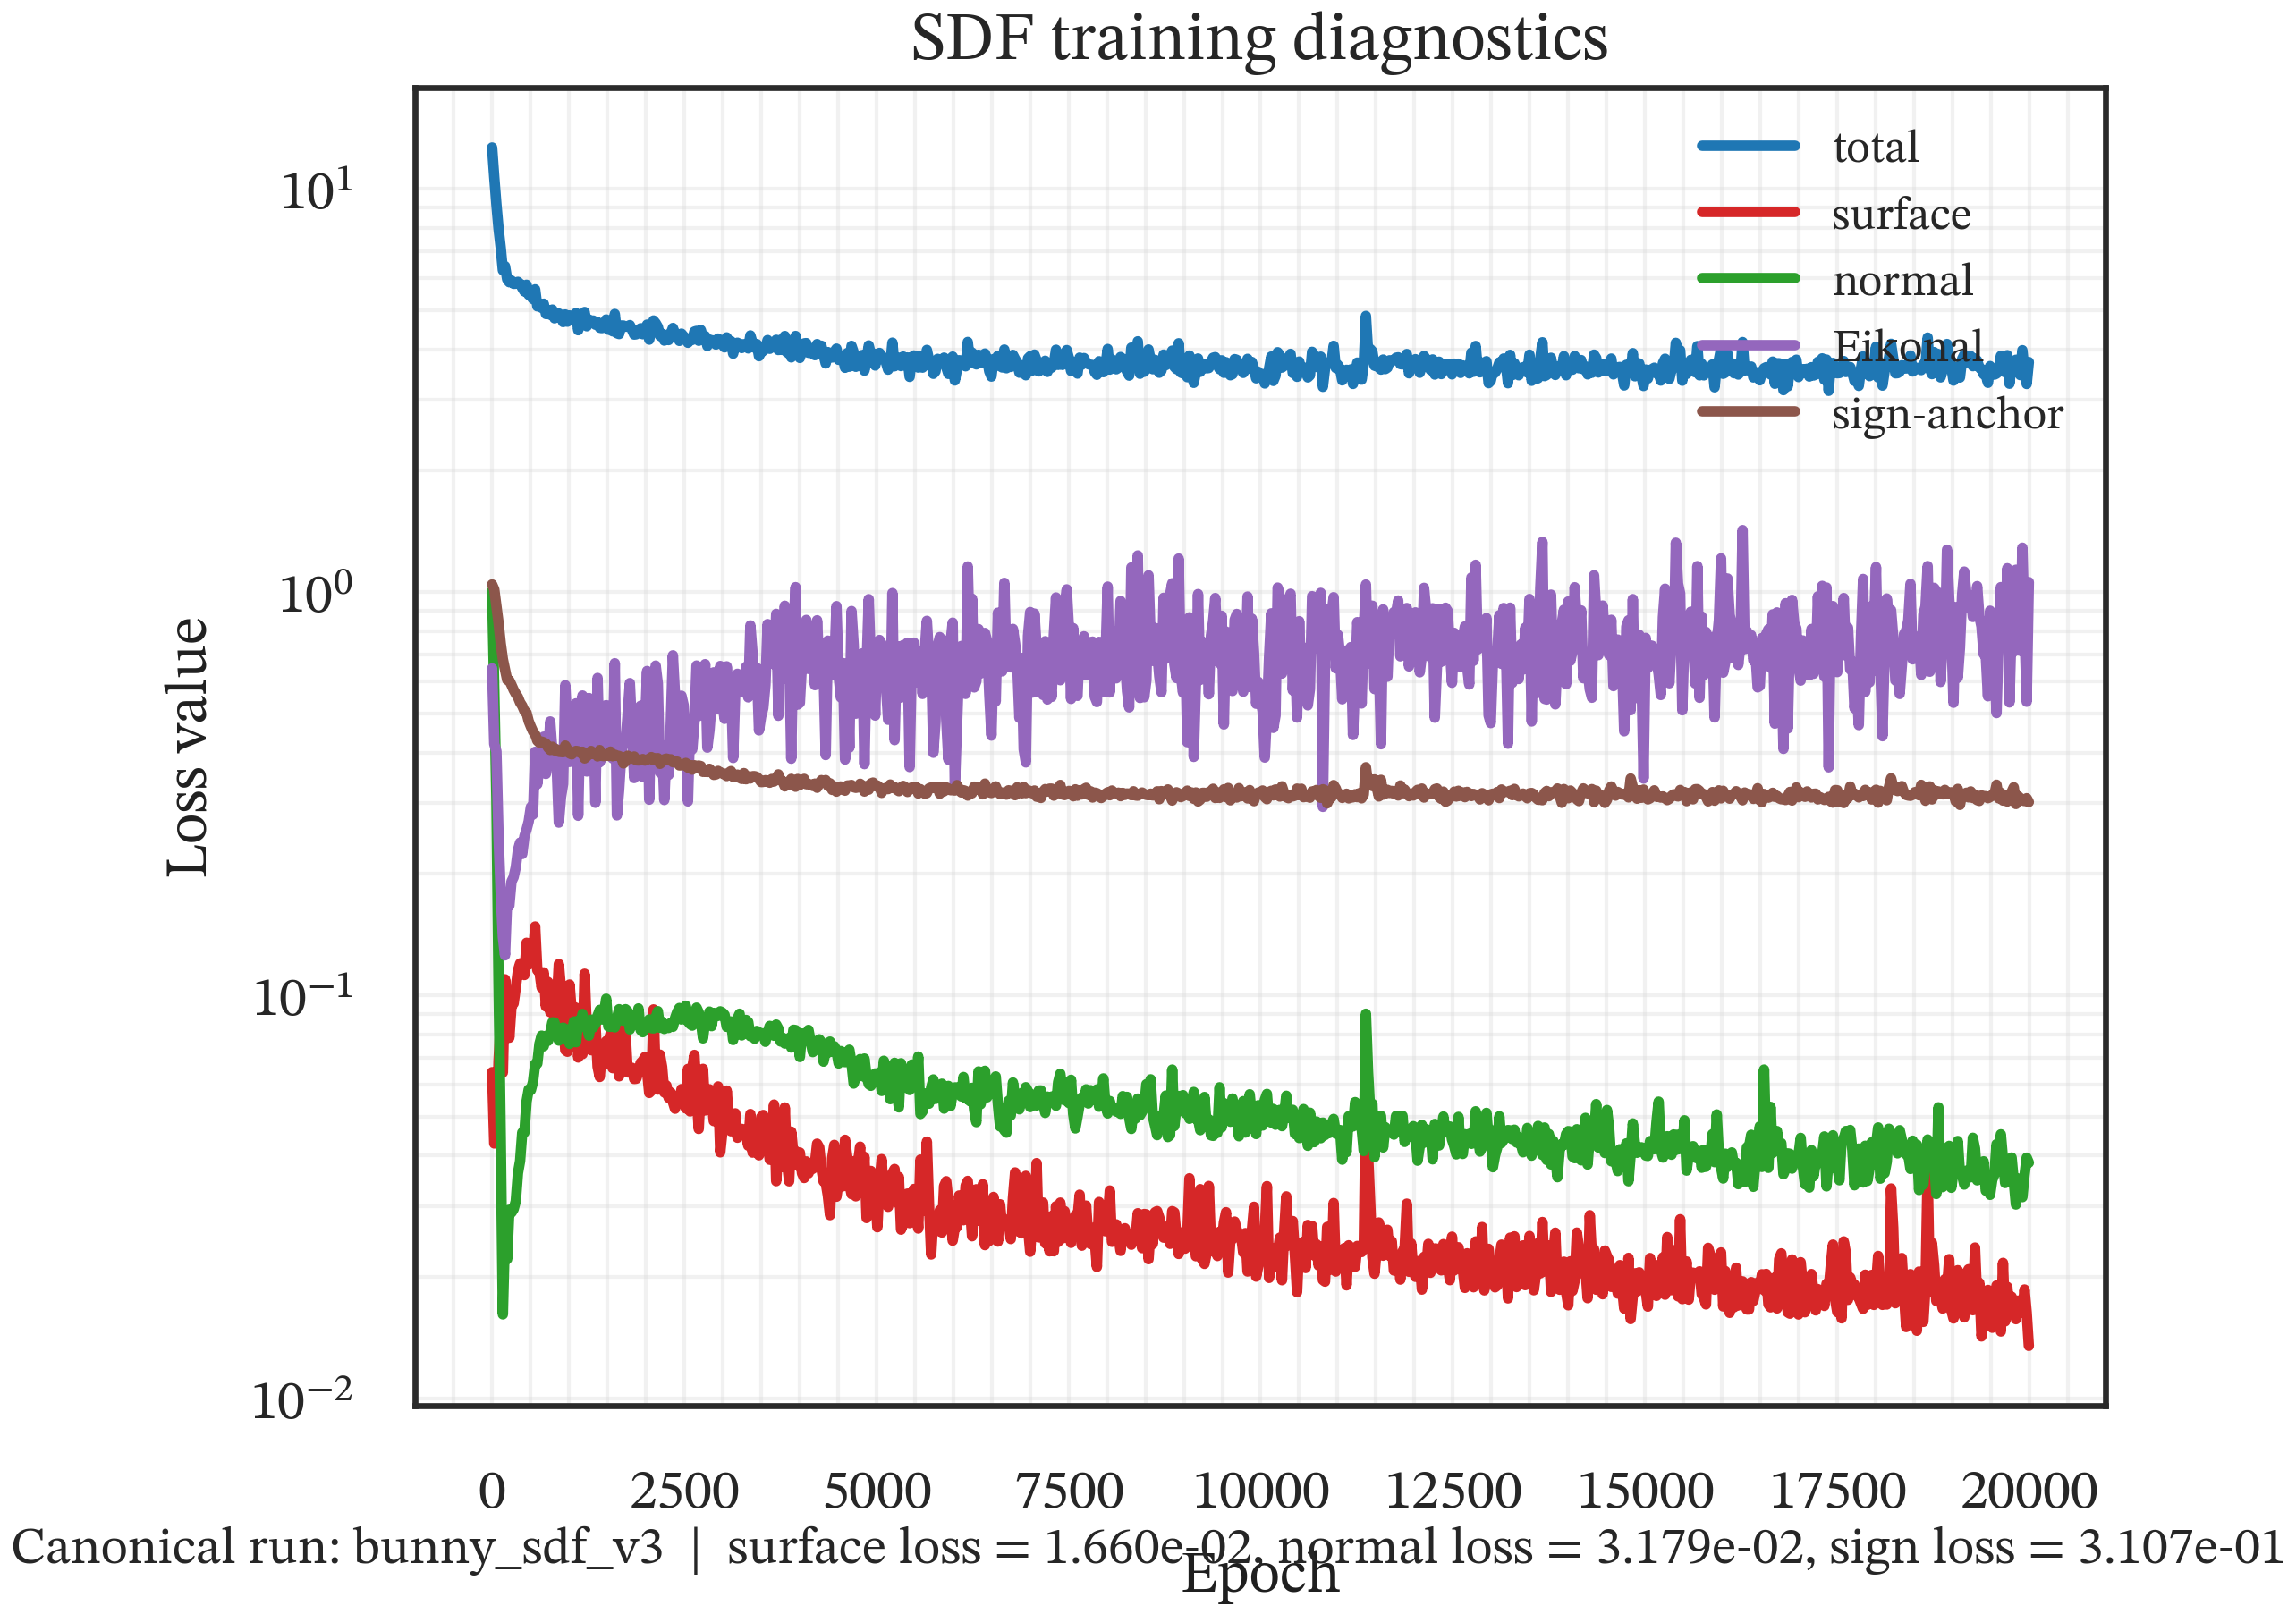
\includegraphics[width=0.97\textwidth]{figures_cmame_core/example3_bunny_sdf/example3_bunny_sdf_learning_pub.png}
\caption{Stanford Bunny volumetric neural SDF benchmark, Part I. Panel (a) shows orthogonal slices of the learned scalar field together with the zero contour, which captures the bulk Bunny geometry. Panel (b) reports the optimization traces for the four training objectives. The main point is that the surface and normal terms decay strongly, while the Eikonal and sign-anchor terms remain the dominant sources of error, so the learned field is more reliable as a surface-capturing volumetric model than as a uniformly accurate signed-distance function.}
\label{fig:bunny_sdf_learning}
\end{figure}

\begin{figure}[htbp]
\centering
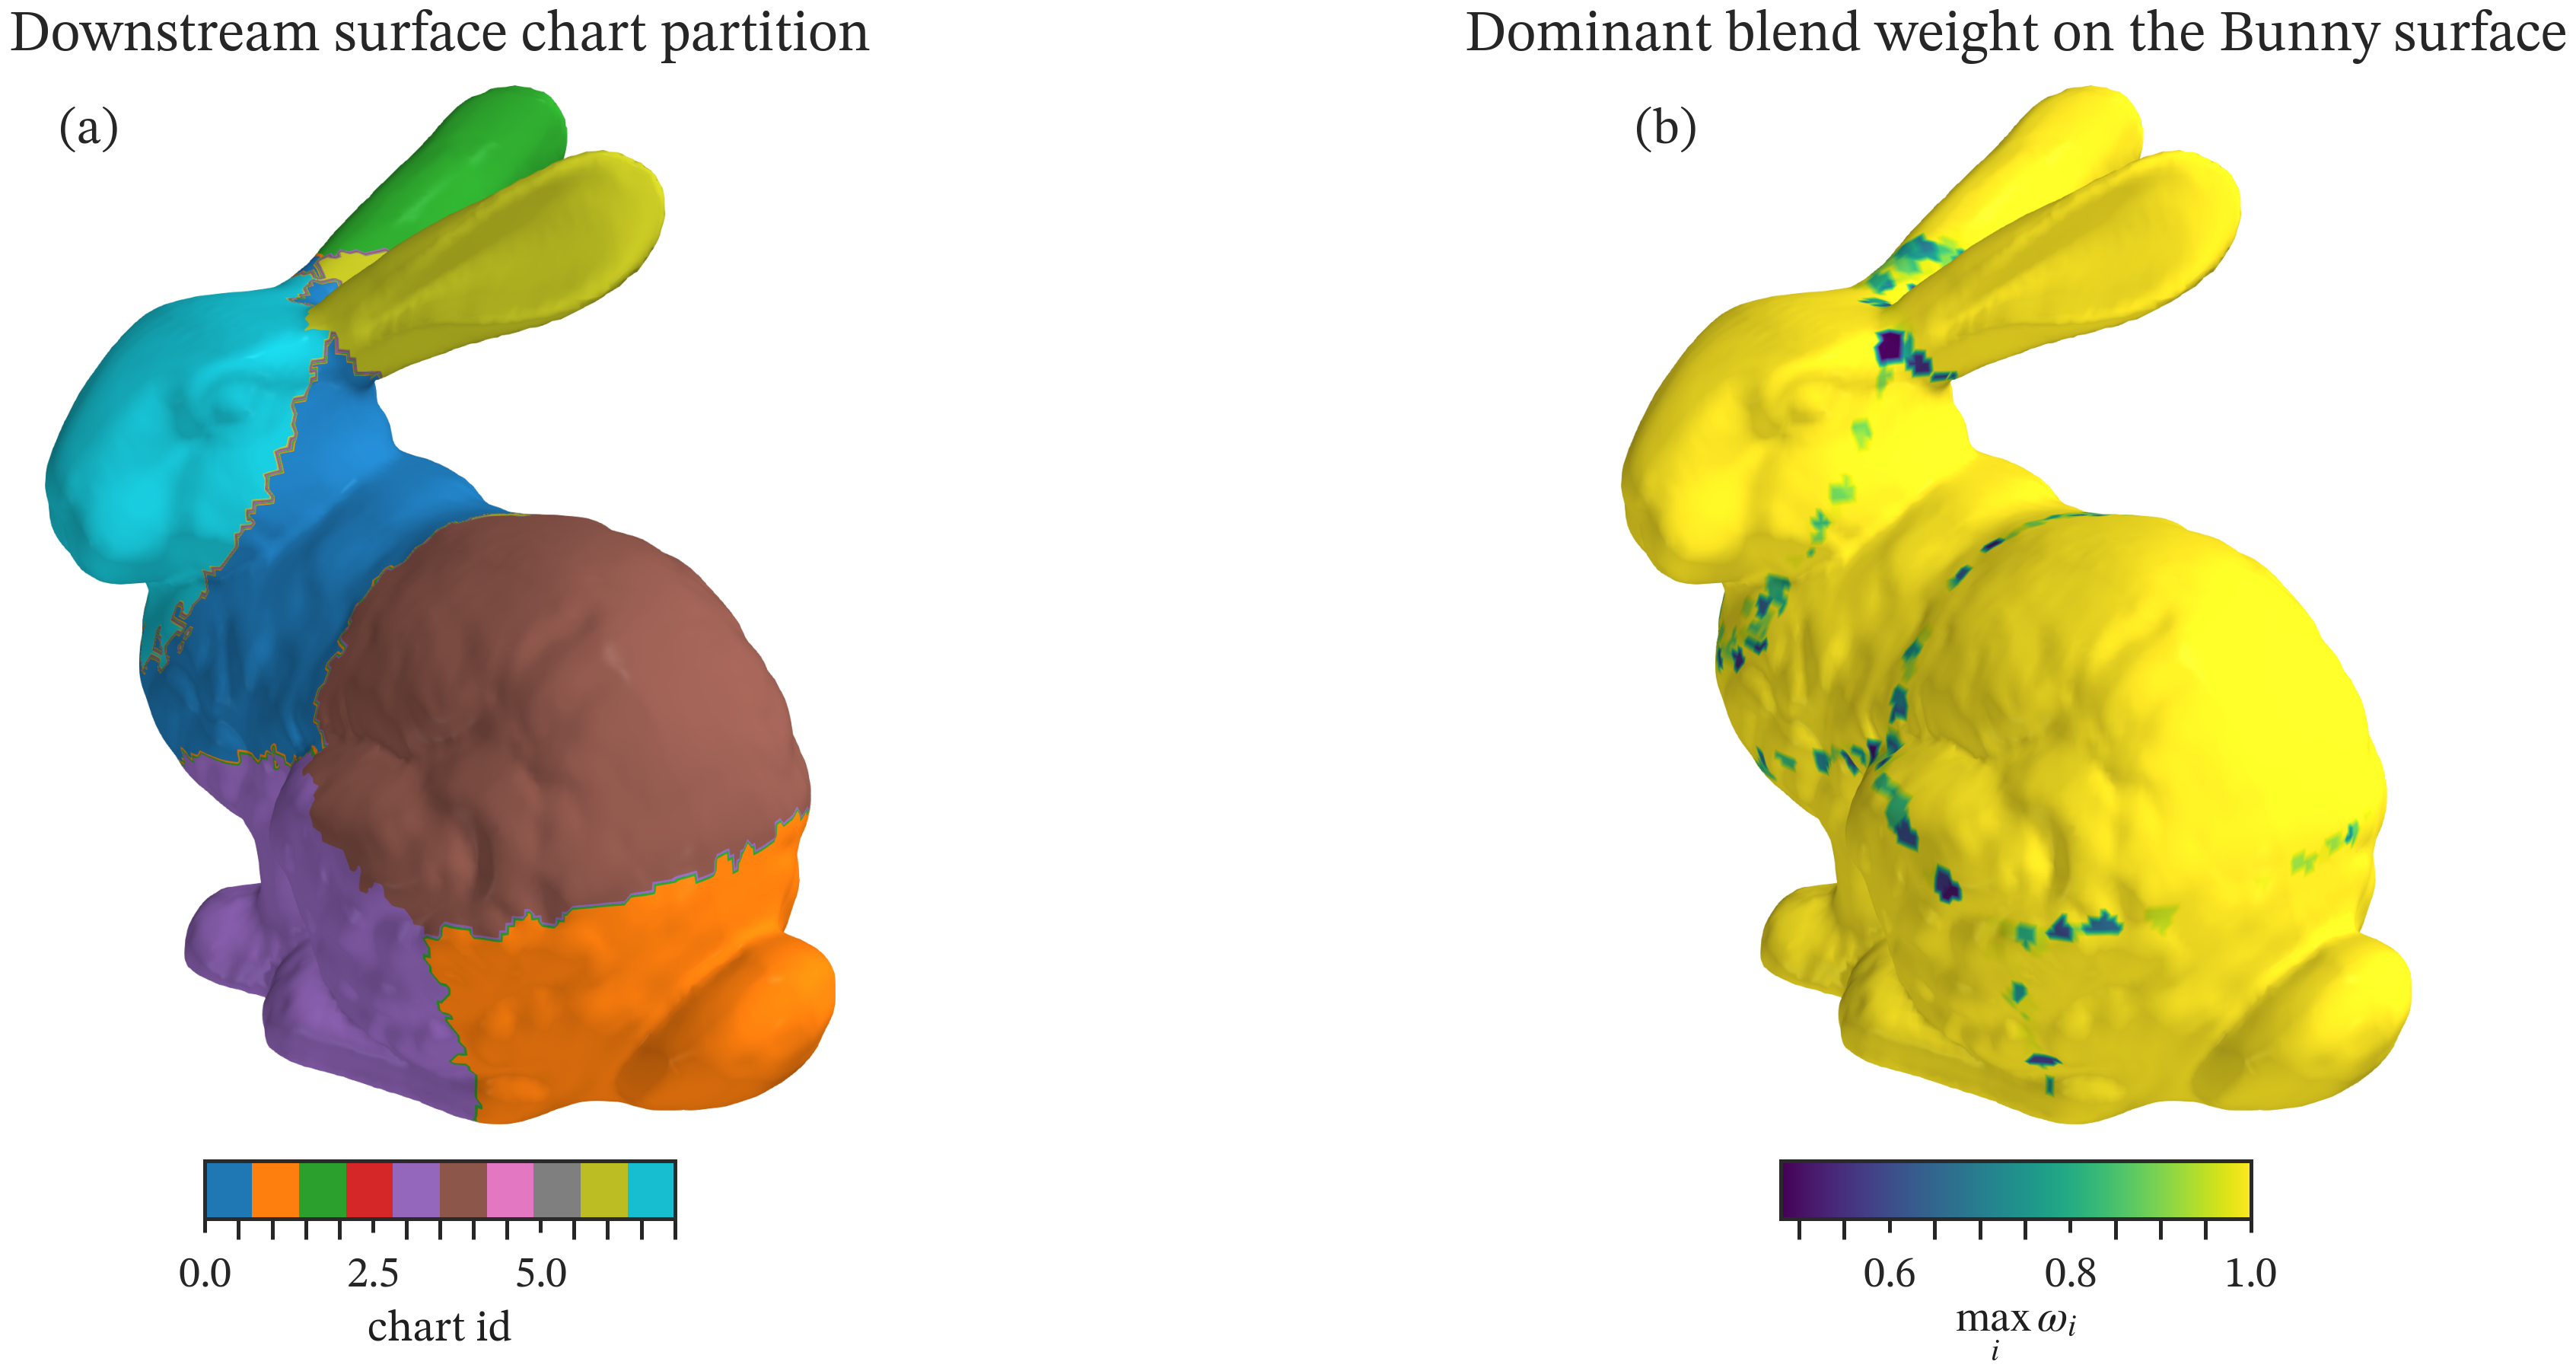
\includegraphics[width=0.97\textwidth]{figures_cmame_core/example3_bunny_sdf/example3_bunny_sdf_surface_pub.png}
\caption{Stanford Bunny volumetric neural SDF benchmark, Part II. The surface visualization is taken from the best archived downstream Bunny Poisson continuation run, \texttt{bunny\_poisson\_8chart\_intpre20k}, so that the chart partition and dominant blend weight are shown on a field-solve artifact rather than on the SDF trainer alone. The chart-partition view shows that the eight charts cover most of the imported PLY surface cleanly, while the dominant blend-weight view shows that the active chart weight remains close to one on most surface points. Together these panels support the qualified claim made in the text: the learned or repaired field is already usable for downstream atlas construction and continuation over most of the geometry, even though thin-feature volumetric ambiguity remains unresolved.}
\label{fig:bunny_sdf_surface}
\end{figure}


% Example 4 source traceability (comment only; not visible in the compiled PDF).
% Paths below are relative to the PINN_coordinate_chart_3Dgeometry/ project root.
% Code:
%   - src/run_torus_inverse_neohookean_atlas.py
%     Main torus atlas-based synthetic inverse benchmark used in the manuscript.
% Data / run artifacts:
%   - runs/torus_inverse_mps/
%     Canonical archived torus inverse run used for the best reported identification metrics.
%   - runs/torus_inverse_mps_dense_v4/
%     Archived torus inverse figure run used for the manuscript field/convergence visualizations.
% Notes:
%   - The torus geometry, prescribed kinematics, and synthetic traction observations are generated analytically inside the code.
%   - There is therefore no external raw-data directory; the run directories contain the generated observations,
%     learned parameters, metric logs, and VTU exports.
\subsection{Example 4: torus synthetic inverse Neo-Hookean identification}
\label{sec:example4}
The original torus inverse script is a controlled synthetic parameter-identification benchmark. Its input is an observed boundary data set
\[
X_{\mathrm{obs}}=\{(x_k,n_k,t^{\mathrm{obs}}_k)\}_{k=1}^{N_{\mathrm{obs}}}\subset \Gamma_{\mathrm{obs}},
\]
where each traction value is generated from a prescribed deformation rather than from an unknown state solve. The point of the benchmark is therefore narrow and deliberate: it tests whether the inverse machinery can recover constitutive parameters when the kinematics are known and the only unknowns are the global material constants.

Let
\begin{equation}
u_{\tau}^{\mathrm{pres}}:\Omega_{\mathrm{torus}}\rightarrow \mathbb{R}^3
\label{eq:torus_prescribed_u}
\end{equation}
be the prescribed torsional displacement field used in the code. From it we construct the deformation gradient
\begin{equation}
\mathbf{F}_{\tau}^{\mathrm{pres}} = \mathbf{I} + \nabla_x u_{\tau}^{\mathrm{pres}}.
\label{eq:torus_prescribed_F}
\end{equation}
The constitutive law is the compressible Neo-Hookean stress
\begin{equation}
\mathbf{P}(\mathbf{F};\mu,K)
=
\mu\left(\mathbf{F}-\mathbf{F}^{-T}\right)
+
K\ln(\det\mathbf{F})\,\mathbf{F}^{-T}.
\label{eq:nh_stress}
\end{equation}
Synthetic traction observations are generated on an observed boundary subset $\Gamma_{\mathrm{obs}}$:
\begin{equation}
t^{\mathrm{obs}}(x)
=
\mathbf{P}\!\left(\mathbf{F}_{\tau}^{\mathrm{pres}}(x);\mu_{\mathrm{true}},K_{\mathrm{true}}\right)n(x),
\qquad x\in \Gamma_{\mathrm{obs}}.
\label{eq:torus_obs_traction}
\end{equation}
The unknowns are the global scalars $(\mu,K)$. In the released code, the traction mismatch is first aggregated through the fixed azimuthal chart weights $\omega_i(x_k)$:
\begin{equation}
\mathcal{L}^{(4)}_{\mathrm{trac}}(\mu,K)
=
\frac{1}{M}\sum_{i=1}^{M}
\frac{\sum_{k=1}^{N_{\mathrm{obs}}}\omega_i(x_k)\,
\left\|
t(x_k;\mu,K)-t^{\mathrm{obs}}(x_k)
\right\|_2^2}
{\sum_{k=1}^{N_{\mathrm{obs}}}\omega_i(x_k)+\varepsilon}.
\label{eq:torus_original_loss}
\end{equation}
The logged total loss in the script is then
\begin{equation}
\mathcal{L}^{(4)}_{\mathrm{tot}}(\mu,K)
=
\mathcal{L}^{(4)}_{\mathrm{trac}}(\mu,K)
+
\lambda_{\det}\,C_{\det},
\qquad
C_{\det}:=
\mathbb{E}_{x\in \Gamma_{\mathrm{obs}}}
\left[
\mathrm{softplus}\!\left(\delta-\det \mathbf{F}_{\tau}^{\mathrm{pres}}(x)\right)^2
\right].
\label{eq:torus_original_total_loss}
\end{equation}
Because $\mathbf{F}_{\tau}^{\mathrm{pres}}$ is fixed by the prescribed kinematics, $C_{\det}$ is constant with respect to $(\mu,K)$. The parameter update is therefore driven entirely by the traction term \eqref{eq:torus_original_loss}, while the determinant barrier is retained in the stored loss history as a kinematic admissibility diagnostic. Chart weights are used only to aggregate observations over azimuthal neighborhoods; this benchmark does \emph{not} solve a chart-local elasticity PDE for the displacement field. Example~4 should therefore be read as a controlled inverse benchmark rather than as a nonlinear field-solve demonstration.

That distinction is precisely why the example matters. By holding the displacement field fixed, the released torus script isolates the constitutive and observation operators and asks whether the inverse machinery can recover the global material constants $(\mu,K)$ from synthetic traction observations. The atlas enters only through eight azimuthal chart weights used to aggregate those observations around the torus; there is no learned displacement field and no chart-local elasticity solve in this benchmark.

For the dense validation run, the optimization starts from $(\mu,K)=(1.746,26.0)$ and converges to $(1.7997,25.0052)$, compared with true values $(1.8,25.0)$. The final relative errors are $1.49\times 10^{-2}\%$ for $\mu$ and $2.09\times 10^{-2}\%$ for $K$, and the traction relative $L^2$ error is $2.09\times 10^{-4}$ after $93.0$\,s. The stored optimization trace strengthens that endpoint evidence: the traction-mismatch term decreases from $2.49\times 10^{-3}$ at initialization to $6.28\times 10^{-8}$ in the final loss history, while the parameter estimates move smoothly into the correct regime. These results support a narrow but important conclusion: constitutive identification is already reliable under known kinematics, which shows that the atlas-based pullback is not limited to Poisson diffusion, even though a full nonlinear chart-local field solve is still beyond the scope of the present benchmark evidence.

\begin{figure}[htbp]
\centering
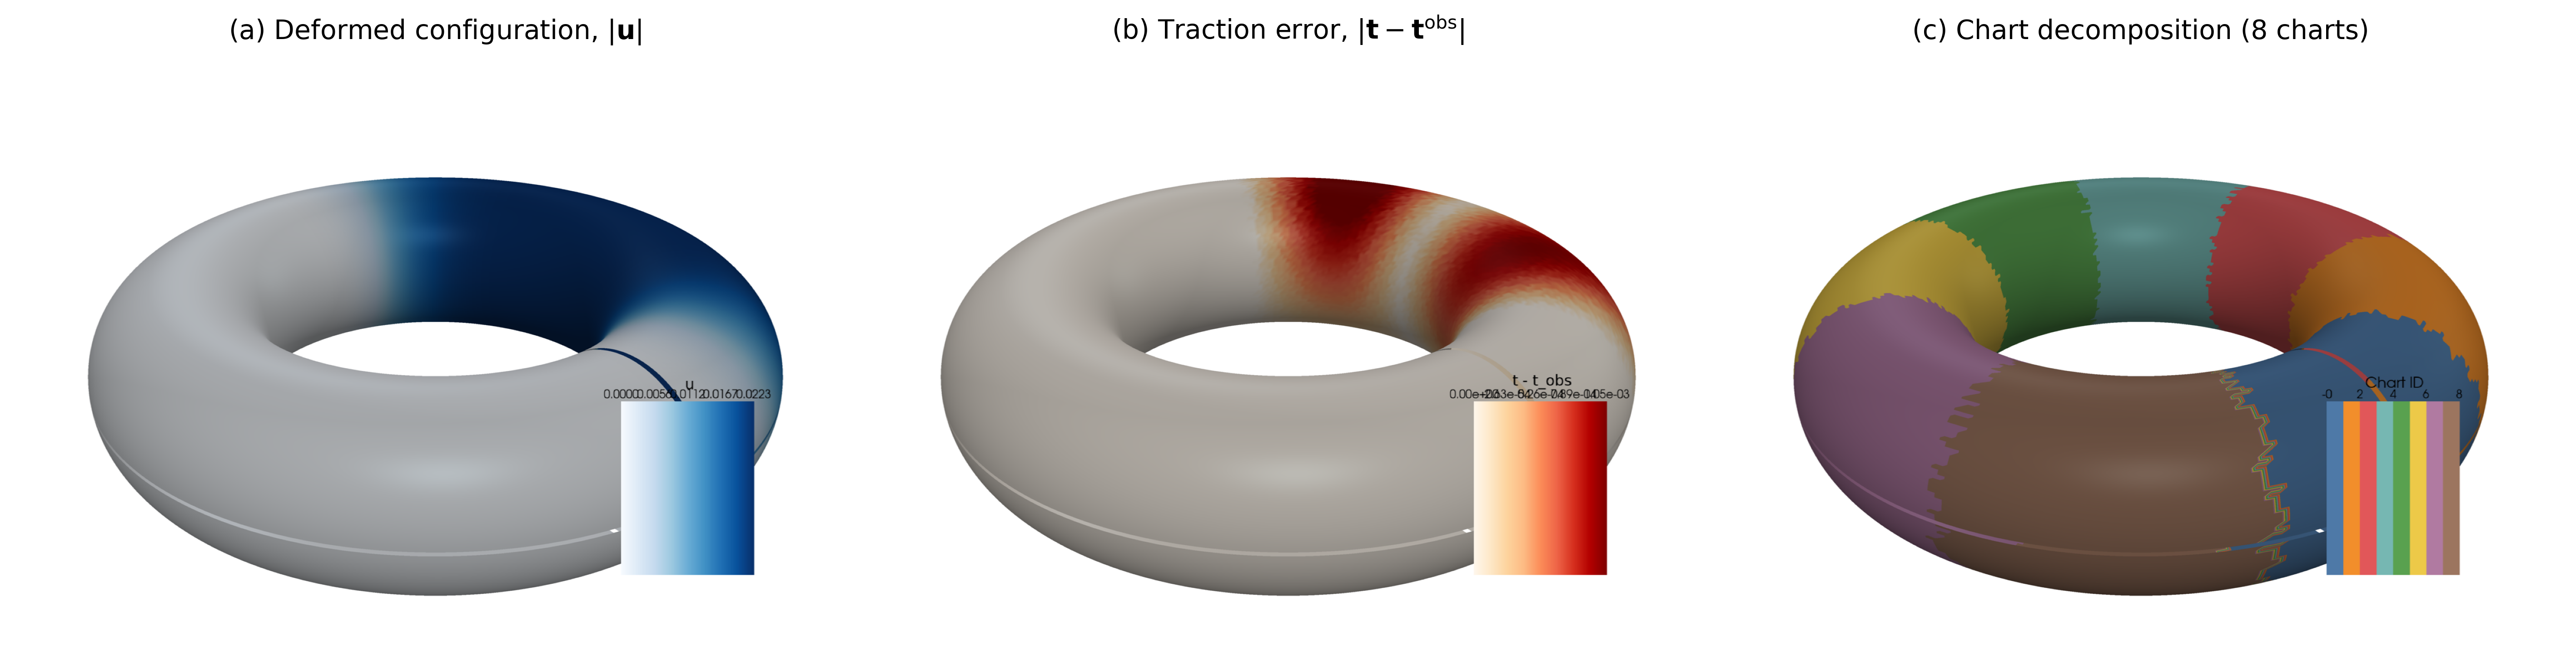
\includegraphics[width=0.98\textwidth]{figures_cmame_core/example3_torus_inverse_original/example3_torus_inverse_fields_pub.png}
\caption{Controlled torus inverse benchmark rendered directly from the dense VTU export of the canonical run. The left panel shows the prescribed deformed configuration colored by displacement magnitude, and the right panel shows the boundary traction-error magnitude on the same geometry and camera. Because the kinematics are prescribed, these panels should be read as diagnostics of the observation fit rather than as evidence of a learned displacement field. The main conclusion is that the traction mismatch remains small and spatially localized over the observed boundary surface.}
\label{fig:torus_inverse_original_fields}
\end{figure}

\begin{figure}[htbp]
\centering
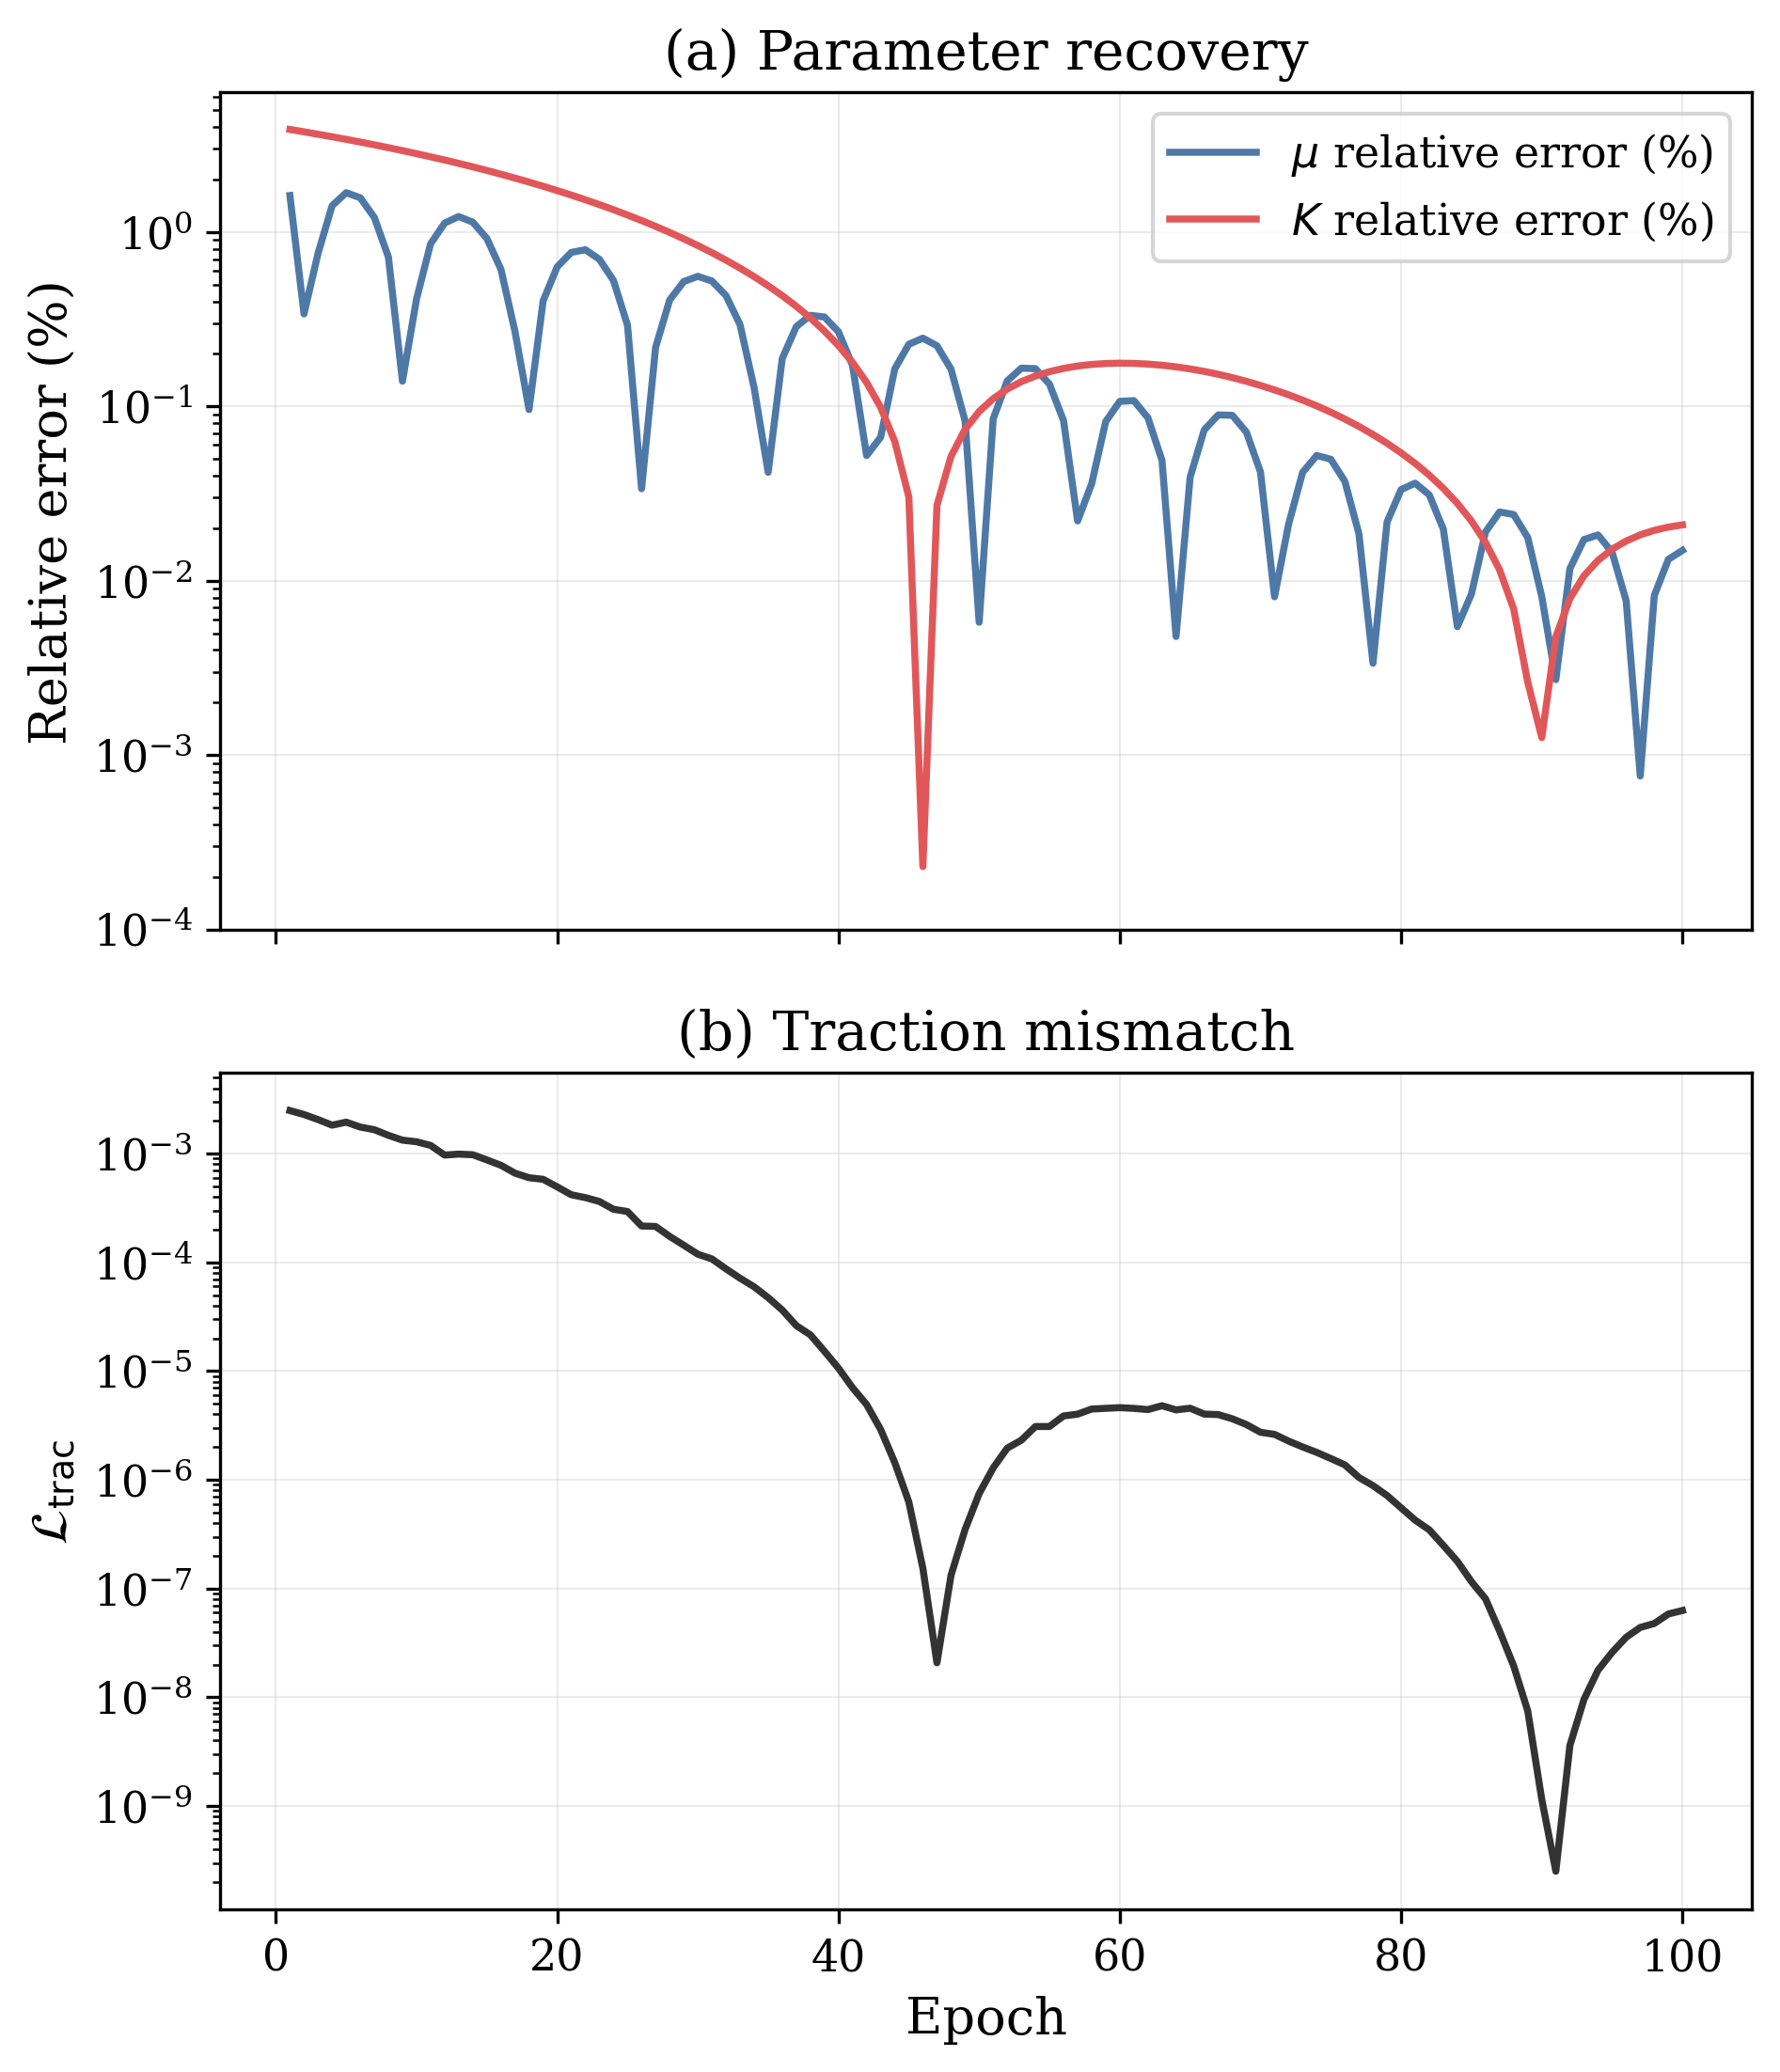
\includegraphics[width=0.62\textwidth]{figures_cmame_core/example3_torus_inverse_original/example3_torus_inverse_convergence_pub.png}
\caption{Parameter-identification history for the dense torus benchmark. The plot shows the relative errors of $\mu$ and $K$ together with the traction-mismatch trace recorded during optimization. The figure supports the benchmark claim in the text: under known kinematics, the inverse trajectory is stable, the parameters converge rapidly into the correct regime, and the traction mismatch decreases to the $10^{-8}$ loss level by the end of the run.}
\label{fig:torus_inverse_original_convergence}
\end{figure}

\subsection{Cross-example comparison and lessons learned}
Taken together, the four examples support a staged numerical argument. The ellipsoid case verifies the mapped operator on analytic geometry; the rabbit benchmark provides the strongest evidence that a fixed atlas plus Schwarz coupling can deliver a forward field solve on complex geometry; the Stanford Bunny benchmark establishes a usable bridge from imported PLY data to a volumetric prior and downstream continuation; and the torus inverse benchmark shows that the same overall infrastructure can already support controlled constitutive identification under prescribed kinematics. The picture is scientifically useful, but it is deliberately narrower than a claim of general dominance over mature meshing plus FEM.

\begin{table}[htbp]
\centering
\scriptsize
\setlength{\tabcolsep}{2.2pt}
\caption{Canonical main-text results organized by argumentative role. The table summarizes what each example supports, the main evidence behind that support, and the main caution that keeps the claim appropriately bounded.}
\label{tab:core_summary}
\begin{threeparttable}
\begin{tabular}{>{\raggedright\arraybackslash}p{2.0cm}>{\raggedright\arraybackslash}p{1.6cm}>{\raggedright\arraybackslash}p{2.35cm}>{\raggedright\arraybackslash}p{2.9cm}>{\raggedright\arraybackslash}p{1.0cm}}
\toprule
Case & Supports claim about & Main evidence & Key caution & Runtime (s) \\
\midrule
Ellipsoid Poisson & mapped-operator verification & rel-$L^2 = 2.26\times10^{-3}$ & analytic geometry only & 106.3 \\
Rabbit Poisson & complex-geometry atlas solve & \shortstack[l]{PINN rel-$L^2 = 2.21\times10^{-2}$\\ FEM rel-$L^2 = 1.79\times10^{-2}$} & \shortstack[l]{PINN uses weak supervision\\ FEM needs $1.48\times10^{6}$ DOFs} & \shortstack[l]{3659\\8395} \\
\shortstack[l]{Stanford Bunny\\ neural SDF} & volumetric geometry learning from PLY data & surface loss $= 1.66\times10^{-2}$ & \shortstack[l]{sign-anchor $= 3.11\times10^{-1}$\\ Eikonal $= 7.29\times10^{-1}$} & ${\approx}4800$\tnote{a} \\
Torus inverse (original atlas) & controlled constitutive identification & traction rel-$L^2 = 2.09\times10^{-4}$ & known kinematics; not a field solve & 93.0 \\
\bottomrule
\end{tabular}
\begin{tablenotes}[flushleft]
\footnotesize
\item[a] Runtime for the Bunny neural SDF is approximate because the training log records wall-clock duration only coarsely; the canonical run required roughly 60--90\,min on the validated hardware backend for 10{,}000 epochs.
\end{tablenotes}
\end{threeparttable}
\end{table}

The cross-example lesson is that mapping and Schwarz are most convincing here as a reusable geometric substrate rather than as a method tied to one discretization. Analytic or learned maps keep the solver in simple reference domains, while local volumetric charts avoid forcing one global parametrization onto geometries that do not admit one cleanly in practice. The rabbit benchmark now validates this claim quantitatively from two independent directions. On the classical side, the atlas-FEM branch recovers the expected $O(h^2)$ convergence---with rates approaching $2.10$ at the finest level---confirming that the mapped Poisson operator, the Schwarz boundary exchange, and the partition-of-unity blending introduce no order-of-accuracy penalty. On the neural side, the compact PINN reaches comparable accuracy with roughly $1.31\times10^{5}$ trainable weights and ${\sim}195$M neural-network evaluations, while the FEM at matched accuracy requires $9.41\times10^{5}$ DOFs but only ${\sim}23$M neural-network queries (for one-time geometric precomputation). The framework therefore does not remove numerical tradeoffs; it changes them in a way that makes the atlas the primary reusable asset, with the local solver choice---neural or classical---determined by whether the application values convergence guarantees or workflow flexibility.





\section{Discussions}
\label{sec:discussion}
The examples in Section~\ref{sec:benchmark_formulations} establish a regime-specific contribution. The archived evidence shows that the atlas workflow is already a credible geometry-first alternative when geometry acquisition, volumetric meshing, or remeshing are themselves the fragile part of the simulation pipeline. It does not show that atlas-based PINNs or atlas-based local solvers should replace mature mesh-based methods whenever a good volumetric discretization is already available.

\subsection{Method-level comparison with alternative workflows}
The FEM baseline transforms the positioning of the atlas formulation from qualitative to quantitative. In conventional finite-element workflows a difficult three-dimensional body is first turned into a volumetric mesh and then coupled to mature local basis functions and linear or nonlinear solvers \citep{de_souza_neto_computational_2011}. The present atlas-based approach replaces the global volumetric meshing step with overlapping chart maps and level-set geometry, and the rabbit FEM baseline now shows concretely that classical FEM can operate \emph{within} this atlas framework with full theoretical convergence: $O(h^2)$ rates approaching $2.10$ at the finest level. This makes the atlas a validated geometric substrate rather than merely a PINN training convenience.

Three specific findings from the rabbit head-to-head merit discussion. First, at matched accuracy the two methods are broadly competitive in wall-clock time ($2{,}939$\,s for FEM at $n=48$ versus $3{,}659$\,s for the compact PINN), indicating that the atlas-plus-Schwarz infrastructure, not the local discretization, is the dominant cost driver. Second, the FEM requires roughly $8.5\times$ fewer neural-network evaluations than the PINN (${\sim}23$M cached versus ${\sim}195$M iterative), because the decoder networks are queried only during one-time geometric precomputation rather than at every training step. Third, the FEM provides a mesh-refinement convergence guarantee that the PINN does not, while the PINN avoids reference-domain mesh generation, stiffness-matrix assembly, and decoder inversion, and extends more naturally to nonlinear operators where matrix reassembly would be required at every Newton step.

The closest PINN alternatives in the literature, such as XPINNs and FBPINNs \citep{shukla2021parallel,moseley2021fbpinns}, also use decomposition to improve training, yet their partitions are primarily algorithmic. In contrast, the present atlas is geometry-first: the same chart structure is used to represent the domain, to generate collocation or quadrature, and to organize Schwarz communication. The rabbit benchmark and its FEM counterpart are the clearest evidence that this idea works in practice, because the same atlas gate report, the same Schwarz iteration, and the same partition-of-unity blending support both neural and classical local solvers with consistent results. The present evidence therefore supports discretization-agnostic geometry representation, not universal accuracy or efficiency superiority.

What makes the contribution mature enough to report now is that the paper validates the geometry representation, mapped PDE operator, and overlap-coupling logic together rather than in isolation, and then stress-tests that geometric scaffold with two fundamentally different local discretizations. The result is not a single benchmark win, but a reusable computational infrastructure whose present strengths and limits are both visible in the archived results.

\subsection{Current limitations and future development priorities}
The repository still contains broader exploratory tracks, but the validated evidence suggests a clear priority order for future work. More ambitious inverse tracks, including the rabbit Elder and Arruda--Boyce variants, remain outside the main-text claims because their stabilization and interface control are not yet as clean as the four validated examples discussed above.
\begin{enumerate}[leftmargin=*]
\item \textbf{Nonlinear forward field solves on fixed atlases.} Example~4 shows that parameter identification under prescribed kinematics is already stable. The more important next step is a genuine atlas-based nonlinear equilibrium solve, so that material nonlinearity, mapped operators, and Schwarz transmission are tested simultaneously.
\item \textbf{Stronger physics-only coupling for the rabbit family.} The rabbit benchmark already passes geometry gates and yields the best complex-geometry forward result in the repository, but it still depends on careful interface weighting, trust-region screening, and guided training design. Reducing that dependence, and eventually removing manufactured guidance from the strongest run, is the most direct route to a cleaner flagship result.
\item \textbf{Thin-feature geometry learning.} The Bunny losses show that near-surface fit is not the binding constraint; sign and Eikonal regularity are. Spatially adaptive importance sampling, local chartwise SDF refinement, and stronger volumetric priors should therefore take priority over simply increasing network size.
\item \textbf{Atlas-based FEM and broader classical baselines.} The rabbit benchmark now includes a direct chart-local P1 FEM baseline, which confirms the expected $O(h^2)$ trend and shows where refinement overtakes the compact PINN. The next step is to extend that comparison to whole-domain meshed FEM, higher-order chart-local elements, and stronger preconditioned Schwarz variants so that the present atlas-based head-to-head can be embedded in a broader classical baseline study.
\end{enumerate}

The paper should therefore be read neither as a rejection of classical meshing nor as a claim that every geometry problem should be solved by atlas-based PINNs. The stronger conclusion is more specific: when geometry acquisition, volumetric meshing, and remeshing are themselves difficult, the released code already demonstrates a credible geometry-first alternative whose present strengths and failure modes are both visible in the stored results.

\section{Conclusions} \label{sec:conclusions}
This paper establishes a geometry-informed atlas framework for boundary-value problems on complex three-dimensional bodies without requiring a global volumetric mesh. The central contribution is an end-to-end computational pipeline in which geometry representation, mapped PDE operators, and inter-chart transmission are designed and validated together. The strongest evidence is the fixed-atlas rabbit benchmark: a validated rabbit atlas supports a complex-geometry Poisson solve, the archived W1--W5 reinforcement study identifies the stabilization mechanisms behind the best PINN result, and the new atlas-based P1 FEM baseline recovers the expected $O(h^2)$ convergence (with rates from $1.45$ to $2.10$) and reaches relative $L^2$ error $1.79\times10^{-2}$ at the finest archived refinement. That head-to-head result shows that the atlas is a reusable geometric scaffold for more than one local discretization family: at matched accuracy the two methods are broadly competitive in wall-clock time, while the FEM requires roughly $8.5\times$ fewer neural-network evaluations (${\sim}23$M cached geometric queries versus ${\sim}195$M iterative training passes) and offers mesh-refinement convergence guarantees that the PINN does not.

The remaining benchmarks define the present scope of that contribution. Analytic ellipsoid verification confirms correctness of the mapped operator, the Stanford Bunny study shows that real PLY data can be turned into a usable volumetric prior and downstream continuation scaffold, and the torus benchmark establishes accurate constitutive identification under prescribed kinematics. Taken together, the results support a bounded conclusion: atlas-based computation is already a credible option when geometry preparation is itself a major numerical burden, but nonlinear forward field solves, stronger thin-feature geometry learning, and broader whole-domain and higher-order FEM comparisons remain open priorities. The durable outcome of the work is therefore a validated geometric scaffold for carrying nontrivial field equations over overlapping volumetric charts.

\appendix
\section{Implementation transparency and hardware backends}
\label{sec:appendix_impl_details}

\subsection{Research workflow and implementation assistance}
The scientific logic of the project remained human-led throughout. The benchmark family, the atlas-based decomposition, the mapped-PDE formulation, the acceptance criteria for validated runs, and the interpretation of success or failure were set by the author. Large-language-model tooling was used only as a low-level implementation assistant for code scaffolding, refactoring, debugging, figure scripting, and artifact packaging. In other words, the assistant accelerated software iteration, but it did not determine the mathematical model, the benchmark scope, or the evidentiary standard required for the manuscript.

\subsection{Hardware backends}
The main text is intentionally hardware-agnostic, but the archived artifacts do retain backend metadata relevant to reproducibility. The canonical rabbit Poisson run \texttt{attempt20c\_compact} records \texttt{device = mps}, \texttt{dtype = float32}, and \texttt{amp\_backend = none} in its metrics file. The canonical torus inverse run \texttt{torus\_inverse\_mps\_dense\_v4} likewise records \texttt{device = mps} and \texttt{dtype = float32}. These entries indicate execution through PyTorch's Metal backend on Apple hardware. The canonical Bunny SDF metadata do not serialize the backend explicitly, so that benchmark is reported in the main text only through its archived loss history and geometry outputs rather than through a device-specific claim.

The codebase itself is broader than any one archived run. Geometry and post-processing utilities include CPU-executable paths, while the rabbit Schwarz solver also exposes optional accelerator-parallel updates for non-overlapping color groups. For blind review, the important point is therefore not one specific workstation but that the manuscript results come from the same PyTorch implementation across Metal, CUDA, and CPU backends, with the concrete backend for a given run recorded in the corresponding artifact whenever that metadata were serialized.


\section*{Acknowledgments}
The author is supported by the Dynamic Materials and Interactions Program from the Air Force Office of Scientific Research, USA, under grant contract FA9550-22-1-0310, and by the United States Army Research Office under grant contract W911NF-24-1-0011.
The views and conclusions contained in this document are those of the authors and should not be interpreted as representing the official policies, either expressed or implied, of the sponsors, including the Army Research Laboratory or the U.S. Government.
The U.S. Government is authorized to reproduce and distribute reprints for Government purposes, notwithstanding any copyright notation herein.

\section*{Declaration of competing interest}
The authors declare that they have no known competing financial interests or personal relationships that could have appeared to influence the work reported in this paper.

\section*{Data availability}
An anonymized artifact package containing scripts, canonical run registries, metric tables, and verification manifests is
provided for peer review as supplementary material. Upon acceptance, the full repository and archived benchmark artifacts
will be released publicly with a persistent DOI. 

\bibliographystyle{unsrtnat}
\bibliography{main}

\end{document}
